% -------------------------------------------------------------------------------------------------
%      MDSG Latex Framework
%      ============================================================================================
%      File:                  main.tex
%      Author(s):             Michael Duerr
%      Version:               1
%      Creation Date:         30. Mai 2010
%      Creation Date:         30. Mai 2010
%
%      Notes:                 - This represents the document root of this template
%                             - Binding correction is 12mm. In case you change this value, you
%                               may also need to adapt the value of \bcorlength in mdsg.sty
%                             - Switch `babel' package options `english' and `ngerman' in case
%                               your thesis is in English
%                             - if you prefer to use utf8 encoding, uncomment the corresponding
%                               line `\usepackage[utf8]{inputenc}' and comment the line
%                               `\usepackage[latin1]{inputenc}'. To compile this example you also
%                               need to include the corresponding introduction example file i.e.
%                               `introduction-UTF8.tex' or `introduction-ISO8859-1.tex'
% -------------------------------------------------------------------------------------------------
%
\documentclass[enabledeprecatedfontcommands,bibliography=totoc,listof=totoc,index=totoc,twoside=true,BCOR=12mm,DIV=12]{scrbook}
%\KOMAoptions{draft=true}                         % uncomment if you want to visualise overful hbox
%\KOMAoptions{chapterprefix=true}                 % uncomment if you like "Chapter" in front of
                                                  % chapter number
\KOMAoptions{appendixprefix=true}                % uncomment if you like "Appendix" in front of
                                                  % appendix number
%\KOMAoptions{...}                                % feel free to add additional KOMA options
%
% =================================================================================================
% set encoding
% -------------------------------------------------------------------------------------------------
%
\usepackage[utf8]{inputenc}                       % uncomment if you prefer utf8 encoding
%\usepackage[latin1]{inputenc}                    % uncomment if you prefer latin1 encoding
%
% =================================================================================================
% load mdsg style
% -------------------------------------------------------------------------------------------------
%
%\usepackage[diplom]{mdsg}                        % uncomment the corresponding option
%\usepackage[fopra]{mdsg}
% \usepackage[bachelor]{mdsg}
\usepackage[master]{mdsg}
%
% =================================================================================================
% initialize macros
% -------------------------------------------------------------------------------------------------
%
\lmutitle{Exploring the Impact of Markets on Multiagent Reinforcement Learning}                       % title: you can force a new line by
%\lmutitle{Titel \\ der \\ Arbeit}                % inserting `\\'. However, this will cause
                                                  % a hyperref warning!
\lmustudentone{Zarah Zahreddin}                    % first author's name
%\lmustudenttwo{Max2 Mustermann2}                 % second author's name
%\lmustudentthree{Max3 Mustermann3}               % third author's name
%\lmustudentfour{Max4 Mustermann4}                % fourth author's name

\lmuprofone{Prof. Dr. Claudia Linnhoff-Popien}    % first supervisor's name
% \lmuproftwo{Prof. Dr. Max Mustermann}             % second supervisor's name
                                                  % (uncomment if not needed)
% \lmuprofthree{Prof. Dr. Max2 Mustermann2}         % third supervisor's name
                                                  % (uncomment if not needed)
\lmuadvisorone{Kyrill Schmid}                    % first advisor's name
\lmuadvisortwo{Robert Müller}                    % second advisor's name
                                                  % (uncomment if not needed)
% \lmuadvisorthree{Betreuer Name3}                  % third advisor's name
                                                  % (uncomment if not needed)
% \lmudraftdate{\today}                             % only for versioning during work!
                                                  % (uncomment for final version!)
\lmudeadline{13. December 2021}                      % deadline (day of submission)
%
% =================================================================================================
% package selection (add additional packages if needed)
% -------------------------------------------------------------------------------------------------
%
%\usepackage{layout}                              % see documentation of this package
\usepackage{cmap}                                 % to produce searchable PDF
\usepackage[T1]{fontenc}                          % split german words with umlaut
\usepackage{lmodern}
\usepackage[english]{babel}                       % for german toc, ...
\usepackage{bibgerm}                              % for german bibliography index
\usepackage{tabularx}                             % more flexible table environment
\usepackage{booktabs}                             % high quality tables
\usepackage{rotating}                             % for generation of landscape tables
\usepackage{multirow}                             % for multirow cells inside tables
\usepackage{amssymb,amsmath}                      % powerful math package
\usepackage[hidelinks]{hyperref}                  % for hyperlinks
\lmuhypersetup                                    % write some pdf properties
\usepackage{flafter}                              % force floats to appear after their reference
\usepackage{subfig}                               % to allow for side by side graphics (subfloats)
\usepackage{pdflscape}                            % enable rotation of landscape pages
\usepackage{hyphenat}                             % proper hyphenation for bla_bla to bla_-bla
\usepackage[all]{hypcap}                          % correct captions
\usepackage{url}                                  % nicer url style
\usepackage{enumitem}                             % for tight lists
%\usepackage{...}                                 % add additional packages here
\usepackage{geometry}
\usepackage{marginnote}
\usepackage{pythonhighlight}

\usepackage[ruled,linesnumbered]{algorithm2e}                            % needed for pseudo code

\usepackage[font=small,labelfont=bf]{caption}
\captionsetup{format=plain,indention=0pt,justification=justified}


\setcounter{tocdepth}{3}                          % sectioning depth in toc
\setcounter{secnumdepth}{3}                       % sectioning depth in text

\graphicspath{{./pictures/}}                      % put all graphics here
% -------------------------------------------------------------------------------------------------
%      MDSG Latex Framework
%      ============================================================================================
%      File:                  hyphenation.tex
%      Author(s):             Michael Duerr
%      Version:               1
%      Creation Date:         30. Mai 2010
%      Creation Date:         30. Mai 2010
%
%      Notes:                 - Instruction \hypenation cannot handle special characters like umlaute
%                               as well as  "a and \"a. Split such words in your text.
%
% -------------------------------------------------------------------------------------------------
%
\hyphenation{Ba-che-lor-ar-}
%\hyphenation{...}                           % further hyphenation examples
                               % this file holds words latex cannot split
%
% =================================================================================================
% start of document
% -------------------------------------------------------------------------------------------------
%
\begin{document}
\setlist{noitemsep}                           % for tight lists
\lmufront                                     % title pages
\newpage
\cleardoublepage
\lmuaffirmation                               % affirmation (work is my own work)
\newpage
\cleardoubleemptypage
\thispagestyle{empty}
\vspace*{2cm}

\begin{center}
    \textbf{Abstract}
\end{center}

\vspace*{1cm}

\noindent A current research question addresses the topic of how to bring mixed-motive agents to work together, in order to achieve a common goal. Mixed-motive describes agents that work independently and whose actions do not affect others directly. However, the agents are not able to communicate. One approach is to introduce markets, namely a shareholder market (SM) and an action market (AM). By using markets, agents gain incentives, when they act cooperatively. Shares of the SM let agents participate in the reward of others and AM enable agents to reward others for certain actions.

This thesis introduces the coloring environment and uses it to compare the application of the two markets in various agent compositions. The coloring environment lets agents move around and color the cells they visit. Visiting a cell that is already colored removes its color. The goal is to color the whole environment.

The rewards of competitive and mixed-motive agents are calculated with the amount of color presence in the environment. Cooperative agents however get one shared reward based on the overall coloration, which can lead to the credit assignment problem (CAP). Additionally, all three compositions face organizational challenges of getting in each other's way. The effectiveness of markets on these problems are analyzed in this research.                        % abstract
\thispagestyle{empty}
\frontmatter                                  % start roman numbering
\tableofcontents                              % toc
\mainmatter                                   % start alpha numbering
%
% =================================================================================================
% place your document text here (take care of encoding)
% -------------------------------------------------------------------------------------------------
%
\chapter{Introduction}\label{sec:Introduction}
% - Motivation \\
% - Goal \\
% - Research Question \\
% - Structure \\

Reinforcement learning (RL) is a popular research topic with many successful and interesting applications. Some popular RL utilizations are in the gaming category, for example Go \cite{sihu16}\cite{sisc17}, chess \cite{batr01}\cite{sihu17}, poker \cite{da01}\cite{xuch21} or very complex player versus player games like Starcraft \cite{viba19} and Dota \cite{bebr19}. Most of the time such applications can be played by multiple agents, either in a team or against each other. 

RL is unique in the fact, that agents learn to solve tasks without prior knowledge. However, having multiple agents try to learn in a shared environment poses several problems. An agent team, i.e. in a soccer game \cite{agtu04}, either score a goal or misses its chance. Retracing the game outcome onto the contributions of all agents and assigning credit accordingly is a common problem called the ``credit assignment problem'' (CAP). 

Other game types, like racing games for example, place players in competitive situations. The common goal is to reach the finish line, the earlier, the better. By using items or strategies, one might start to sabotage others, in order to place first. Although, when time becomes a factor, the goal might shift to finishing as quickly as possible, instead of wasting time disrupting others. Players still compete but keep a neutral behavior towards each other, since the success of one does not affect the achievement of others. This composition is further called mixed-motive. Cooperative, competitive and mixed-motive agent constellations are referred to as compositions.

Mixed-motive and competitive situations can be applied or recreated with RL. However, training competing agents often leads to disorder, since they get in each other's way or become greedy and self-centered. A new research showed, that adding incentives to mixed-motive agents enabled cooperative behavior and helped to align individual goals among each other. Schmid et al. \cite{scbe21} achieved this through a neutral market. A shareholder market (SM) allows agents to sell shares and let others participate in their success. Action market (AM) is the alternative option and lets agents buy specific actions from others. The following outline presents application details and the research question of this thesis. 

\section{Research Question}

Since markets were only applied and analyzed on mixed-motive agent compositions so far, it leaves the question open, how the problems of cooperation and competitive compositions would be affected by them. By using markets on cooperation settings one could assume, that agents with higher results contributed positively to the common goal. Therefore, the credit should already be assigned accordingly. In theory, markets in competitive compositions should also improve the results. Through the incentives, the individual goals of agents might be aligned, which should reduce the competitive behavior.

This research therefore compares the effectiveness of each market applied on all three compositions. Furthermore, to get a bigger picture agents will be trained with two different learning algorithms and the results will be compared. To enable the research of different compositions, this thesis further introduces the coloring environment. Agents have unique colors and can stand or move in a grid. Agents that move around color the visited cells. However, moving on a colored cell removes the color instead. The different compositions are modeled through a reward schema, which signalizes how good or bad the coloration result is. 

Cooperating agents always get the same reward among each other, based on the overall coloration. In mixed-motive compositions, agents only get reward based on their own contribution. Competitive settings are similar to mixed-motive, but the difference here is, that agents can take over colored cells of their opponents. The ending condition of the environment is a fully colored grid.

The training of the agents is executed through the two most popular learning algorithms of RL: proximal policy optimization (PPO) and the training of a deep Q-Network (DQN). PPO is a policy gradient method, that allows agents to enhance their decision-making. DQN is an algorithm that utilizes a neural network together with Q-values. Q-values evaluate all possible actions of a situation and chooses the best option in regard to possible future outcomes.

Comparing the affects of shareholder and AMs in three distinct compositions and using two different learning algorithms results in many executions. To get an overview, scoreboards will be presented that filter the three best trainings, with or without markets, of each composition and algorithm. Based on those scores the beset settings will be challenged in more difficult setups with more agents, to see how well they can scale.

\section{Thesis Structure}
The structure of the thesis begins by covering the background of this research question. First, the definition of RL is presented, and then the two learning algorithms PPO and DQN are introduced. Next comes the related works Chapter, which first analyzes the credit assignment problem in detail and introduces the most common solution for it. Markets are the second topic here, and entails all calculations and trading conditions. 

Chapter \ref{sec:Approach} shows the implementation details of the coloring environment, its reward calculations and implementation details of the two learning algorithms and markets. The training results are displayed in the Chapter \ref{sec:Results} and discussed afterwards. To conclude this research the results are summarized and extensions or changes for future research are suggested.
\chapter{Background}\label{sec:Background}
- Describe the technical basis of your work \\
- Do not tell a historical story - make it short

\section{Reinforcement Learning}
%https://lilianweng.github.io/lil-log/2018/02/19/a-long-peek-into-reinforcement-learning.html#key-concepts
\marginpar{rl components}
Sutton and Barto wrote in ``Reinforcement learning: An introduction''\cite{suba18} that Reinforcement learning (RL) is based on two components that interact with each other: an environment and an agent, see Figure \ref{fig:rl_cycle}. Those interactions take part during a time period with discrete timesteps $t\in\mathbb{N}_0$ until a goal is reached or the ending condition applies. Formally the journey of the agent finding the goal state is described as the Markov Decision Process (MDP) and every method that leads the agent there is a reinforcement learning method. When multiple agents act in the same environment the Markov decision process is called a stochastic game \cite{buba10}.
% Initially the agent gets a starting environment state $S_0$, and can processes it to choose and execute an action $A_0$. This concludes the first time step. The environment changes based on the action and transitions into the next state $S_{1}$. In return the the agent receives the new state with a reward $R_{1}$ rating the action $A_0$. Afterwards the agent proceeds to execute actions which leads to the displayed cycle of Figure \ref{fig:rl_cycle}.
\begin{figure}[hpbt]
    \centering
    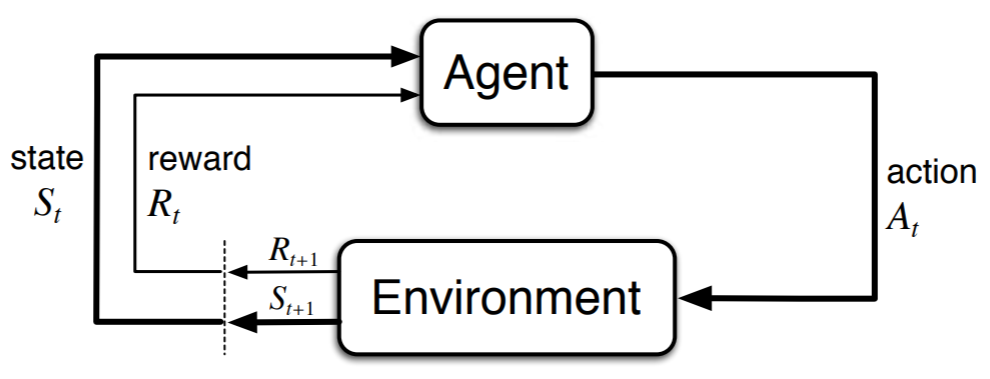
\includegraphics[width=0.6\textwidth]{pictures/RLInteractionSB}\\
    \caption[Reinforcement Learning Cycle]{The cycle of agent-environment interaction as
        shown in ``Reinforcement learning: An introduction''\cite{suba18}}\label{fig:rl_cycle}
\end{figure}

\marginpar{sets and values}
The state $S_t$ is part of a set $S$ containing all possible environment states. Since its likely that not all actions are valid in each environment state the agents action selection is based on a restricted set $A_t\in A(S_t)$. In a multiagent environment however, every agent chooses its action and adds it into a joint action set, which is executed collectively on the environment \cite{buba10}. The reward $R_t$ is element of a set of possible rewards $R$, which is a subset of real numbers $R \subset \mathbb{R}$. Therefore, the reward can potentially be negative or very low to emphasize a bad action. The general concept of RL, as defined by Sutton and Barto, is to maximize rewards. Thus, unlike machine learning approaches the agent starts with no knowledge about good or bad actions and enhances the decision-making by aiming to improve the reward.

\marginpar{policy}
Sutton and Barto continue by defining the agents action selection with respect to the current state as a policy $\pi$. They explain further that a policy could be as simple as a lookup table, mapping states to actions or it could contain a complicated search process for the best decision.
In most cases however, policies return actions with assigned percentages for the current state.
During environment interactions agents gain rewards, which then can be used to update the policy accordingly. For example, should the reward be low or negative it could be interpreted as a penalty. In return the policy $\pi(a \mid s)$ could then be adapted to change to a very low probability for that action in combination with that certain state. So next time the agent finds itself in that state the bad action is not very likely to be chosen again.

\marginpar{value function}
While rewards only rate the immediate situation, a value function, i.e. the state-value function $v_{\pi}(s)$ for a policy $\pi$, can be used to estimate the long-term value of a state $s$. The result is the total accumulated reward an agent could get following that state and choosing actions based on the current policy. States that offer immediate high reward could end in
% The value function is of importance, due to states bringing high rewards could end in
low reward streaks. In the opposite case, a low reward state could subsequently yield high rewards. Therefore, value functions are of great use to achieve the maximum reward.
% Other value functions can also take the executed
% action into account to reach the state from which the rewards are estimated.

\marginpar{exploration vs exploitation}
The last part to note about RL is that it entails the problem of balancing exploration and exploitation. In order to learn, an agent has to explore the options given. However, since maximizing rewards is the goal an agent could become greedy and exploit its knowledge by choosing actions of which it knows to result in small but positive rewards. If an agent doesn't explore enough the best action sequence will stay hidden. Whereas when an agent always explores without exploiting its knowledge, chances are that the reward will not be optimal.

\section{Proximal Policy Optimization}
\marginpar{intro}
In 2017 Schulman et al. introduced the concept of Proximal Policy Optimization (PPO) in
the article ``Proximal Policy Optimization Algorithms''\cite{scwo17}.
This section is solely based on that article in order to explain the Algorithm.
Policy optimization is the improvement of the action selection strategy $\pi$ based on the
current state $s_{t}$. This is achieved by rotating two steps: 1. sampling data from the policy and 2.
optimizing that data through several epochs.

\marginpar{TRPO, Advantage func}
The origin of PPO lies in a similar approach called Trust Region Policy Optimization (TRPO).
TRPO strives to maximize the following function:
\begin{equation}\label{TRPO}
    \underset{\theta}{maximize}\,\hat{\mathbb{E}}_{t} [\frac{\pi_{\theta}(a_{t} \mid s_{t})}{\pi_{\theta_{old}}(a_{t} \mid s_{t})}
    \hat{A}_{t}-\beta \, KL[\pi_{\theta_{old}}(\cdot \mid s_{t}),\pi_{\theta}(\cdot \mid s_{t})]]
\end{equation}
with $\hat{A}_{t}$ as an estimator of the advantage function. The advantage function often calculated with the
state-value function $V(s)$, a reward $r$ and a discount coefficient $\lambda$ over a period of Time $t$
\begin{equation}\label{advantage}
    \hat{A}_{t} = -V(s_{t})+r_{t}+\lambda r_{t+1}+ \ldots + \lambda^{T-t+1} r_{T-1} + \lambda^{T-t} V(s_{T})
\end{equation}

The fraction in the Minuend of \eqref{TRPO} can be replaced by
$r(\theta)$ %= \frac{\pi_{\theta}(a_{t} \mid s_{t})}{\pi_{\theta_{old}}(a_{t} \mid s_{t})}$
and represents the probability ratio of an
action in the current policy in comparison to the old policy, with $\theta$ being a policy parameter.
The result of $r(\theta)$ is greater than
one, if an action is very probable in the current policy. Otherwise the outcome lies between zero and one.
Schulman et al. further describe that TRPO maximizes the "surrogate" objective
\begin{equation}\label{TRPO surrogate}
    L^{CPI}(\theta) = \hat{\mathbb{E}}_{t}[ \frac{\pi_{\theta}(a_{t} \mid s_{t})}{\pi_{\theta_{old}}(a_{t} \mid s_{t})} \hat{A}_{t}]
    = \hat{\mathbb{E}}_{t}[r(\theta)\hat{A}_{t}]
\end{equation}
However, maximized on its own without a penalty this results in a large outcome and leads to drastic
policy updates.

\marginpar{problem TRPO}
In order to stay in a trust region, as the name suggests, a penalty is subtracted from the
surrogate function \eqref{TRPO surrogate}.
The penalty is the Subtrahend of equation \eqref{TRPO} and contains the fixed coefficient $\beta$.
Regardless of the function details and outcome of $KL$, the coefficient $\beta$
is hard to choose, since different problems require different penalty degrees. Even in a single problem
it could be necessary to adapt the coefficient, due to changes within the setting.

\marginpar{PPO}
Therefore Schulman et al. introduced
\begin{equation}\label{PPO}
    L^{CLIP}(\theta) = \hat{\mathbb{E}}_{t}[\min(r(\theta)\hat{A}_{t},clip(r(\theta), 1-\epsilon, 1+\epsilon)\hat{A}_{t})]
\end{equation}
which is very similar to \eqref{TRPO} but does not require coefficients.
The first part of $\min$ contains $L^{CPI}$ \eqref{TRPO surrogate}.
The second part contains a $clip$ function which narrows the space of policy mutation with
the small hyperparameter $\epsilon$. After applying the clip function $r(\theta)$ lies between
$[1-\epsilon,1+\epsilon]$. Calculating the minimum of the clipped and unclipped probability ratio
produces the lower bound of the unclipped $r(\theta)$, preventing the policy to change drastically.
%[TODO ???]

\marginpar{PPO Algo}
PPO is defined by the following equation
\begin{equation}\label{PPO Algorithm}
    L_{t}^{CLIP+VF+S}(\theta) = \hat{\mathbb{E}}_{t}[L_{t}^{CLIP}(\theta) - c_{1}L_{t}^{VF}(\theta) + c_{2}S[\pi_{\theta}](s_{t})]
\end{equation}
with $c_{1}$ and $c_{2}$ as coefficients. The authors point out that the loss function \\
$L_{t}^{VF} = (V_{\theta}(s_{t})-V_{t}^{targ})^2$
combines the policy surrogate and the value function error term and is
necessary once a neural network shares parameters between policy and value function.
Finally an entropy bonus $S$ is added to ensure exploration.
Schulman et al. continues to show an example of an Algorithm using PPO, see Fig. \ref{fig:ppo_algo_code}.
$N$ detonates (parallel) actors collecting data in T timesteps in each Iteration.
Afterwards the policy is optimized in K epochs by computing the Loss function \eqref{PPO Algorithm} on the
corresponding $NT$ timesteps of data, using a minibatch.
\begin{figure}[hpbt]
    \centering
    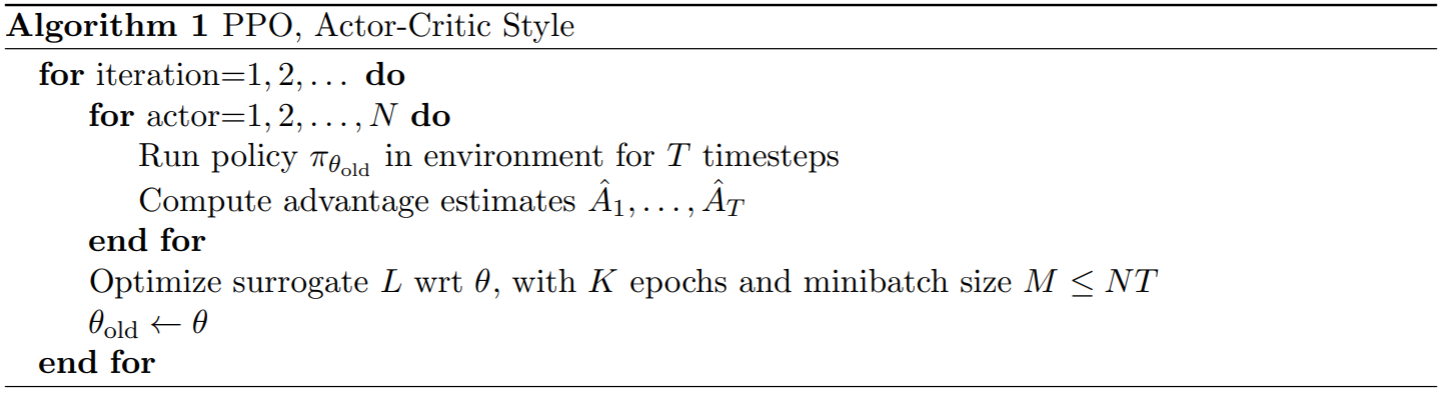
\includegraphics[width=1\textwidth]{pictures/ppo_algo_code.png}\\
    \caption[Exemplary Use Of PPO]{Exemplary use of PPO, as shown in ``Proximal Policy Optimization Algorithms''\cite{scwo17}}\label{fig:ppo_algo_code}
\end{figure}

\section{Deep Q-Learning}
% -------------------------------------------------------------------------------------------------
%      MDSG Latex Framework
%      ============================================================================================
%      File:                  introduction-[UTF8,ISO8859-1].tex
%      Author(s):             Michael Duerr
%      Version:               1
%      Creation Date:         30. Mai 2010
%      Creation Date:         30. Mai 2010
%
%      Notes:                 - Example chapter
% -------------------------------------------------------------------------------------------------
%
\chapter{Related Work}\label{sec:RelatedWork}
% - Definition of field of research \\
% - Scientific Scope \\
% - Which comparable work in research exists? \\
% - Separation from other works
\marginpar{intro and comp. problems}
Realistic RL scenarios often involve multiple agents solving problems together, for example robots working in warehouses and factories. Such multiagent environments come with many difficulties. On one hand in a scenario where agents work independently, it is very probable that they get in each other's way. They aim to achieve the highest score or finish their individual tasks, preventing the overall goal to be achieved.

\marginpar{coop problems}
In cooperative environments on the other hand, agents share the reward and therefore can not tell who contributed useful actions. 
%Hence, all agents receive the same reward regardless of their contribution, which aggravates learning.
The independence problem is discussed in chapter \ref{market} whereas the cooperation challenge is the focus point of the next chapter.

\section{Credit Assignment Problem}\label{CAP}
\marginpar{coop and problem}
Sutton and Barto \cite{suba18} define a RL environment as cooperative, when agents execute their actions collectively each time step but receive one overall reward in return. In this case, individual learning is difficult or even impossible. Collective actions may contain bad choices that would be rewarded or, in case of a penalty, good actions that would be punished. Deciding which agent deserves more or less of the common reward is referred to as the credit assignment problem (CAP) \cite{mi61}.

\marginpar{CAP definition and kinds}
The CAP originated in a one-agent environment that only returned reward once the goal is reached or the terminating condition applied. A popular example of this is a chess game. In 1961, Minsky \cite{mi61} elaborated on this by explaining that a player wins or loses the game, but cannot retrace which decision got him there. Later on, Sutton decomposed the CAP into subproblems, namely the structural and temporal CAP \cite{su84}. He suggests, that the temporal problem lies in assigning credit to each chess move by determining when the position improves or worsens, rewarding or penalizing that certain action. On the contrary, the structural CAP is assigning credit to the internal decision that leads to each particular action.

\marginpar{CAP multi}
% Sutton also refers to a chess game to explain the subproblems. 
Transferring the single-agent CAP into a multiagent environment Agogino and Tumer \cite{agtu04} imply that the problem shifts from being of temporal to structural type. They explain that while a single agent faces the temporal CAP due to many steps taken within an extended time period, in the multiagent case it becomes a structural CAP because of multiple actions in a single-time-step. Since the actions are executed all at once, the problem is now evaluating the decision that lies underneath.
% They explain that a single agent faces the temporal CAP when many steps are taken within an extended time period so learning from the returned reward at the end is problematic. Whereas in the multiagent setting it becomes a structural CAP because of multiple actions leading to a shared reward during a single-time-step.

\marginpar{cap solution dr}
Over the years many solutions and theories emerged in order to solve CAPs in multiagent environments \cite{rabe09}, \cite{zhli20}, \cite{agtu04}. A popular example for a simple approach to solve the problem is the difference reward (DR) \cite{ngku18}, \cite{yltu14}, \cite{agtu04}. The idea is to calculate the overall reward with the joint multiagent actions as always. In order to find the DR $D_i(z)$ for an agent $i$, the following function applies:
\begin{equation}\label{dr}
    D_i(z) = G(z) - G(z_{-i})
\end{equation}

The first part of the equation $G(z)$ represents the overall reward. This reward is the result of the collective action set of one time step, containing the actions of all agents. The second part $G(z_{-i})$ demonstrates the result of the same actions and time step, excluding only the action of agent $i$. Another approach to find the DR is to select a default action in $G(z_{-i})$ for the analyzing agent $i$, instead of dropping its action completely \cite{vega96}.

Calculating the difference between the two rewards results in the difference reward $D_i(z)$ of agent $i$. A high DR indicates a lucrative action of the analyzing agent, since excluding its action or picking something else leads to a small subtrahend. With this method each agent has the opportunity to learn how their actions contribute to the global reward, enabling individual learning. 

\section{Markets}\label{market}
\marginpar{intro mixed motive}
As described earlier, agents that share an environment and act independently can often hinder each other from reaching the common or individual goal. Sutton and Barto defined a game to be competitive, when agents receive varying reward signals \cite{suba18}. In most cases agents follow a mixed-motive, meaning that their individual rewards could sometimes align and sometimes be in conflict. An environment is purely competitive, when the increase in reward of one agent leads to reward decrease of the others.

\marginpar{SMG details}
Schmid et al. introduced in ``Stochastic Market Games'' \cite{scbe21} concepts adding incentives when agents act cooperatively in mixed-motive settings to improve the overall rewards for all participants. The idea of a Stochastic Market Game (SMG) is to enable dominant cooperative strategies through a global and impartial trading market. A stochastic game becomes a SMG if two conditions are met. First, the environment actions of agents are extended with market actions. Second, the reward function adjusts the calculated rewards based on agreements met in the market executions. Furthermore, Schmid et al. defined two types of markets: unconditional and conditional markets.

\marginpar{sm}
They compare the concept of unconditional markets to companies and shareholders, since shareholders do not need to fulfill any conditions to receive the dividends. In unconditional SMGs both companies and shareholders are agents that buy and sell shares as market actions. Figure \ref{fig:sm} shows such a shareholder market (SM). During each time step, every agent has the possibility to put their share on the market or to announce a buying offer directed to another agent.

\marginpar{sm transaction}
If the buying offer coincide with a share that is up for sale in the same step, a market transaction is registered. Now, the shareholder participates in the reward of the transaction agent by a fixed dividend $d$. Schmid et al. mention that an optional price $p$ can be defined as a price a seller receives from the buyer upon each share purchase. They claim however, that agents with high rewards are very likely to gift their shares in order to align the goals of the other agents with their own. Shareholders profit from the success of the selling party through the dividends.

\marginpar{am}
On the contrary, the authors define conditional markets similar to purchase contracts, where buyers pay a fixed price $p$ to sellers when they in turn meet the buyers demand. A proposed conditional SMG is the so-called action market (AM). In this case actions are extended with a buying offer, containing one expected action from one specific agent, see figure \ref{fig:am}.

% Illustations of conditional and unconditional markets, as defined in ``Stochastic Market Games''\cite{scbe21}}
% \label{fig:multipic}

\begin{figure}[hpbt]
    \centering
    %%----start of first subfigure----
    \subfloat[Shareholder market (taken from ``Stochastic Market Games'' \cite{scbe21})]{
        \label{fig:sm} %% label for first subfigure
        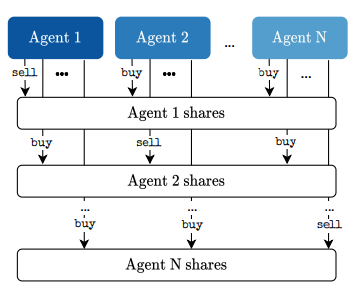
\includegraphics[width=0.48\linewidth]{pictures/SMG_sm.png}}
    \hspace{0.01\textwidth}
    %%----start of second subfigure----
    \subfloat[Action market]{
        \label{fig:am} %% label for second subfigure
        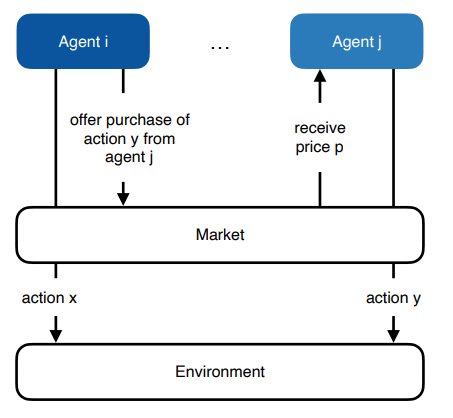
\includegraphics[width=0.41\linewidth]{pictures/SMG_am.png}}
    \caption[Illustrated Markets]{Illustrated Markets as defined in ``Stochastic Market Games'' \cite{scbe21}}
    \label{fig:multipic} %% label for entire figure
\end{figure}

\marginpar{transactions by chance}
In both market settings a purchase is established if the specified agent happens to execute a selling action that matches with a buyer. It is important to emphasize that the matching is performed each time step, leaving it to chance, whether purchases take place. Hence, in case of an action market agents do not know in advance if and what action another agent could be buying from them. Despite this uncertainty, the researchers showed, that both market implementations yielded promising results. An increase of the overall rewards of participating agents in mixed-motive games was seen.
% -------------------------------------------------------------------------------------------------
%      MDSG Latex Framework
%      ============================================================================================
%      File:                  introduction-[UTF8,ISO8859-1].tex
%      Author(s):             Michael Duerr
%      Version:               1
%      Creation Date:         30. Mai 2010
%      Creation Date:         30. Mai 2010
%
%      Notes:                 - Example chapter
% -------------------------------------------------------------------------------------------------
%
\chapter{Approach}\label{sec:Concept}
This Chapter introduces the RL components of this research, namely the coloring environment and its agents. Since, the aim here is to execute learning with markets in various multiagent scenarios, the implementation of the three agent compositions: cooperation, mixed-motive and competitive is shown in Section \ref{env}. The compositions are tightly coupled with reward distribution, which is why Section \ref{reward_calculations} covers the detailed implementation of reward calculations. Furthermore, the process of learning and how the two algorithms PPO and DQN were implemented is the topic of Section \ref{learning_process}. Lastly, the two market implementations and their influence on the rewards are discussed in Section \ref{market_settings}.

\section{Coloring Environment}\label{env}
% Introduce Gridworld, Agent actions, goal etc.
A RL environment is a versatile and unbiased instance, that can in this case visualize changes and agent behavior.
% Although a human visualization is optional, agents need to have some sort of understanding what state they are acting in. 
In figure \ref{fig:env}, the environment used in this work is presented. It originated from an openAI project called ``Minimalistic Gridworld Environment'' \cite{chwi18}, which is designed for one agent whose main goal is to solve labyrinth puzzles. However, for the purpose of this research, the environment is changed heavily, becoming the ``Coloring Environment''. Multiple agents can act in the new instance to try and achieve a common goal - to color all walkable cells.

\begin{figure}[hpbt]
    \centering
    %%----start of first subfigure----
    \subfloat[Human visualization of the coloring environment. A dot represents one agent. Cells change their color when agents move on them.]{
        \label{fig:env} %% label for first subfigure
        \includegraphics[width=0.35\linewidth]{pictures/Gridworld}}
    \hspace{0.01\textwidth}
    %%----start of second subfigure----
    \subfloat[Simplified agent observation of the current environment state. The number one represents a colored cell.]{
        \label{fig:bin_env} %% label for second subfigure
        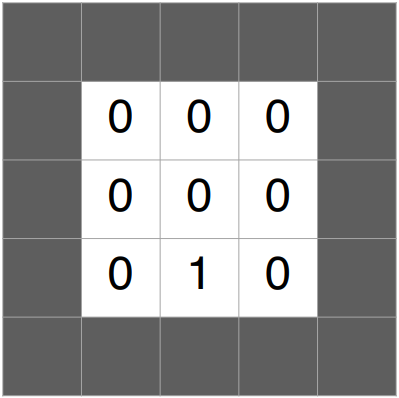
\includegraphics[width=0.35\linewidth]{pictures/binary_gridworld}}
    \caption[Coloring Environment]{Representations of the coloring environment}
    \label{fig:multipic_env} %% label for entire figure
\end{figure}

In the visualization \ref{fig:env} the outer dark cells show walls and the white cells are floors. The agent is represented with the red dot and the cell on which it is located is marked with the same color. By moving on the available space the agent can color more cells.  Every environment cell holds information about the object type it represents, being either walls, floors or agents. Furthermore, each object class contains information about its current color, whether it is accessible for an agent and, in case of a floor tile, if it is colored. Figure \ref{fig:bin_env} shows a simplified environment observation an agent processes each time step.

Floor cells manage the coloration state in binary form, as displayed in \ref{fig:bin_env}, with a one signalizing that the cell is colored. The environment reacts to agent movements by coloring the cells they visit. The environment is successfully solved, once all fields are colored. Otherwise, agents loose by using up a limited amount of steps. If a cell is already in coloration state one and an agent walks over it again the bit is switched, and the cell is reset to zero, removing its color. Besides moving up, down, left and right an agent can also execute the action wait, to stay in place.

\subsection{Compositions}

When multiple agents are placed in the coloring environment together, there are several ways how they will behave towards each other. Depending on the setting, even the environment distinguishes how certain actions affect the state. Per default agents will try to work together, to reach the environment goal. Alternatively, they could work independently or even compete with each other.

Each agent has a different random color. Cells adopt the color of the agent that walks over it. The primary focus in cooperative agent compositions however, is only the binary state. The agents always receive the same reward, regardless of the colors on the grid. An extreme example here would be one agent that colors the whole environment on its own. Naturally, this would result in a high reward and for cooperation this means that all other agents would get the same amount. 

In a DR setting however, agents are able to estimate their contribution, in order to improve their actions. This implementation executes the default action wait to find $G(z_{-i})$, see equation \eqref{eq:dr}. By choosing wait as the default action, agents can learn what the environment outcome and general coloration percentage would be if they had not participated in the current step. It is important to note here, that DR settings are always an extension of the cooperation mode and are never used together with other compositions and markets.

% The opposite is the case in competitive scenarios. 
In mixed-motive settings the colors are of importance. Agents only gain rewards based on their individual contributions. Thus, the rewards are generated by looking up each percentage a color is present and assigning that value to the same colored agent as reward. For example if a red agent colored 60\% of the grid red the reward for that agent would be 0.60. 

In a fully competitive mixed-motive scenario the reward calculations stay the same, only disabling the bit switching for opponent colors. Therefore, agents can directly capture already colored cells when they walk over them. However, if the cell contains the same color as the agent that moved on it, it is reset instead. Therefore, taking over the cells of the opponents is beneficial, since it increases the presence of the own color, leading to a higher reward.

In comparison, the basic mixed-motive composition shows no advantages resetting colored opponent cells. Instead, cell resets are always punished with a small negative reward, regardless of the composition. Hence, it is not likely that the agents work against each other in mixed-motive compositions, yielding a neutral or independent behavior between agents.

\subsection{Observation}
The observations agents receive from the environment are always generated from their individual point of view, with them in the center. The observation only contains a restricted area around them, making the environment a partially observable MDP. In large environments this feature increases the difficulty.
%but at the same time reflects the reality. 
An example for an observation of an agent is shown in \ref{fig:agent_obs}. This observation depicts the internal state of the environment visualization of image \ref{fig:env}.

\begin{figure}[hpbt]
    \centering
    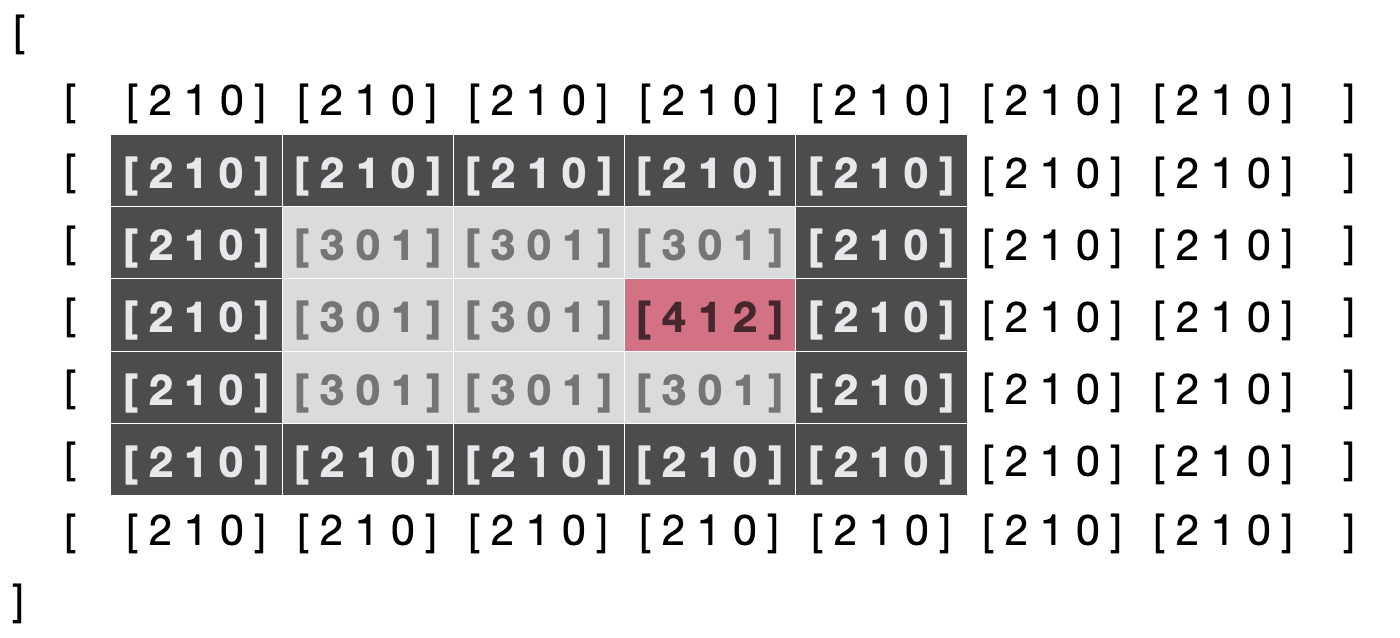
\includegraphics[width=0.8\textwidth]{pictures/agent_observation}\\
    \caption[Agent Observation]{The internal agent observation}\label{fig:agent_obs}
\end{figure}

Per default the agent has a view size of a seven by seven grid, represented in a three-dimensional array, similar to a picture with RGB information. Here, all highlighted entries are part of the grid that is shown in Figure \ref{fig:env} and the red array shows the agent. The first dimension of the observation array contains the whole internal observation of an agent. The second array dimension represents the environment grid. Since the view size of the agent exceeds the dimension of the 5x5 visual grid, the additional rows and columns are filled with placeholders, in this case walls. All highlighted row entries can be mapped to the columns of \ref{fig:env}, starting from the top left of the visualization. The last dimension contains cell information, which is always composed of three elements. 

% This also reduces the complexity of checking for a fully colored grid by just looking at all coloration states, regardless of the object type.

The first cell element defines the object type with one being just an empty cell, two shows a wall, three a floor tile and four an agent. The second element stores the coloration status, showing whether a cell is colored, with zero signalizing an uncolored cell. Since agents can not walk onto walls, represented as $[\;2\;1\;0\;]$, that object type always has a coloration state of one. The third cell encoding describes the color of a cell. To better distinguish the types in the visual representation, walls are zero for the color black and floors are initially white with encoding one. Each agent is assigned a number from two upwards which in turn stands for a randomly generated RGB color. The Floor color encoding is overwritten with the agents color code when the cell is captured. For example, should the agent move to the left, the cell of the previous position is now a colored Floor cell $[\;3\;1\;2\;]$. The new position of the agent is row three and column four with cell encoding $[\;4\;1\;2\;]$.

\section{Reward Calculations}\label{reward_calculations}
The allocation of rewards is closely related to the composition of the agents, which can be specified by the user in training or visualization runs. In addition, the environment shape can be set, a number of agents placed and more. A basic example command for a training run is shown in listing \ref{lst:command}.

\begin{lstlisting}[float=htp,caption=Exemplary command to execute training with three agents in a coloring environment using PPO as algorithm,label=lst:command,language=bash, numbers=left, numberstyle=\tiny, numbersep=8pt ,xleftmargin=3ex,xrightmargin=1ex]
$ python -m scripts.train
    --algo ppo
    --model ppo-training
    --env Empty-Grid-v0 
    --grid-size 7
    --agents 3 
    --max-steps 20
    --setting mixed-motive
\end{lstlisting}

The \verb|--algo| parameter can be either ``ppo'' or ``dqn'' to choose a learning algorithm. This argument is the only required setting for training. All other configurations, including those not listed in \ref{lst:command}, have default values and are shown in Appendix \ref{ax:training_params}.
%  discussed in the Sections \ref{learning_process} and \ref{market_settings}. An overview of all training parameters and their default values is listed in .
With \verb|--model| the destination path is defined, in which all logs, recordings and status updates are stored. Line 4 and 5 configures the environment. In alternative to the empty grid option of \verb|--env|, as shown in figure \ref{fig:env}, four homogeneous rooms can be generated with ``FourRooms-Grid-v0'' to increase the difficulty. The rooms are always of the same size and each room is accessible to all adjoining neighbors by one wall opening, which is random and changes in each episode. The overall size of the grid is set in Line 5. However, all grids in every layout option have outer walls that narrow the area in which agents can move. Hence, in a grid of size seven the agents can only move in a five by five field, due to the surrounding walls.

The amount of agents that act in the environment is set through the argument \verb|--agents| and the maximum quantity of steps they can execute is defined with \verb|--max-steps|. To gain the highest reward, the agents need to color the whole field before they run out of steps. Lastly, the argument \verb|--setting| specifies the composition of the agents. If no setting is set the agents work cooperatively. In the example of \ref{lst:command} the setting ``mixed-motive'' is chosen. The last two options here are ``mixed-motive-competitive'' and ``difference-reward''. % and ``percentage''.

Regardless of the composition, agents initially generate separate rewards in each step based on their individual environment change. For instance, agents that color a field produce a positive reward of 0.1, whereas agents that reset a field contribute a penalty of negative 0.1. Agents that just wait generate a reward of zero. The only exception is the setting ``mixed-motive-competitive'', since agents can capture opponent cells. If that is the case they get a positive reward of 0.1 otherwise the rules stay the same. 

Rewards are always written into a list, which is initially returned by the environment, see algorithm \ref{algo:step_reward}, line 1. The position in the list indicates the accountable agent, i.e. a reward list of $[0.1, 0, \cdots ]$ shows that agent zero is responsible for a reward of 0.1 and so forth. In algorithm \ref{algo:step_reward} the update process of the initial environment rewards during each step is summarized. This step function takes the training arguments of Appendix \ref{ax:training_params} into account, which leads to the four conditions below.

\begin{algorithm}[H]
    \DontPrintSemicolon
    observations, rewards, done, info = environment.step(actions)\;
    \;
    \uIf{difference reward setting} {
        rewards = calculate difference reward for each agent
    }
    \ElseIf{cooperative setting}{
        rewards = calculate one cooperative reward
    }
    \;
    \If{market specified}{
        rewards = execute market actions and return transaction rewards\;
    }
    \;
    \If{done}{
        rewards = calculate final rewards
    }
    \;
    \textbf{return} observations, rewards, done, info\;
    \caption{Reward calculation each step}\label{algo:step_reward}
\end{algorithm}

The first condition checks for a ``difference-reward'' setting. In this case, the agents work in cooperation but try to solve the CAP by calculating the DR, see function \eqref{eq:dr}. To achieve that, the current reward array is summed up, to summarize the overall reward. As a result the variable $G(z)$ of the DR equation is now set to the sum. To find the subtrahend of the equation, the agents are iterated, and their individual calculations take place. Here, the environment rewards are added up again, but this time the reward of the current agent is set to zero. This sum is the value of $G(z_{-i})$ for agent i. The function \eqref{eq:dr} is now applied for each agent and the initial reward list is updated with the individual DRs. 

The last step of the DR reward update is checking, whether any value exceeds an upper or lower bound. If that is the case then the value  is set to the corresponding limit. Otherwise, the reward stays as is. The upper and lower bounds are necessary, due to more participating agents possibly leading to a really big or very small sum. For example, very large sums without bounds could in turn decrease the importance of the final reward for reaching the environment goal. The other extreme are high negative sums demotivating agents to move. The bounds in this implementation are set to 0.1 and -0.1.

If the setting is set to the standard cooperation, the reward needs to be changed to a new homogeneous value for each agent, since they share the outcome. Again, the sum of the initial environment reward is calculated and reassigned to each agent position in the rewards array. The values must be clipped again in the same procedure as for the DR values. Here however, all rewards of the array are changed to the same clipped value, should the bounds be exceeded. Settings that contain ``mixed-motive'' skip all previous reward updates, since in this case each agent keeps their individual value.

As third condition the market argument is checked for a SM or AM. In this case the market transactions changes the rewards. Details of the market process are discussed in Section \ref{market_settings}. One thing to note here is, that agents can execute market transactions in each step. For example, they can spend their current reward on actions or shares that are for sale or receive the purchase price from buyers, which in turn modifies the rewards.

The last condition depends on the done flag which signalizes the end of an episode. The environment sets done to true, once either the grid is fully colored or the maximum step amount is reached. In this case, the final reward calculations are applied, see algorithm \ref{algo:final_reward}. The current rewards are passed as an argument to this calculation, since the list is modified again. %The result of those calculations is the final update of the reward variable.

\begin{algorithm}[H]
    \DontPrintSemicolon
    \eIf{mixed in setting}{
        \For(){each agent}{
            rewards[agent] += agent color percentage on the grid
        }
    }{// cooperative setting \;
        rewards += overall coloration percentage of the Grid
        
        \If {difference reward setting} {
            rewards = calculate difference rewards
        }
    }
    \;
    \If{market specified}{
        rewards = final market adjustments executed on rewards
    }
    \;
    \textbf{return} rewards\;
    \caption{Final reward calculation}\label{algo:final_reward}
\end{algorithm}

During the final reward calculations, the different agent compositions are checked again. In a ``mixed-motive'' or ``mixed-motive-competitive'' setting, each agents' grid coloration percentage, based on their color presence, is added to the individual reward. Otherwise, the composition is based on cooperation and the general grid coloration, regardless of the colors, is looked up and added to each reward value. 

Additionally, the presence of a DR setting needs to be checked here. For the final DR calculations the environment supplies information in the \verb|info| variable of algorithm \ref{algo:step_reward} Line 1. Namely, what the general coloration percentage of the environment would be for each agent, if this agent had executed action wait. Those percentages are subtracted from the cooperative coloration percentage to generate the DRs. Finally, the last market calculations are taken into account, see Chapter \ref{market_settings} for details.

\section{Learning Process}\label{learning_process}
In order to compare different settings and agent compositions easily, each agent manages its own learning improvement, observation and action selection. Therefore, all calculations and estimations are executed independently, for instance policy updates and value estimations. They also set up their own neural networks and optimizers and update them only with their own values. However, the environment still connects the agent experiences, by reacting to all agent actions simultaneously in each step and including visible agents in the observation.

Depending on the learning algorithm the corresponding class is instantiated by the training script, as shown in Figure \ref{fig:training}. The PPO and DQN classes both extend a base class that provides some abstract methods and a multiprocessing operation to execute actions on several environments at once. The base class returns data, allowing the training script to create recordings and log files to enable evaluation.

\begin{figure}[hpbt]
    \centering
    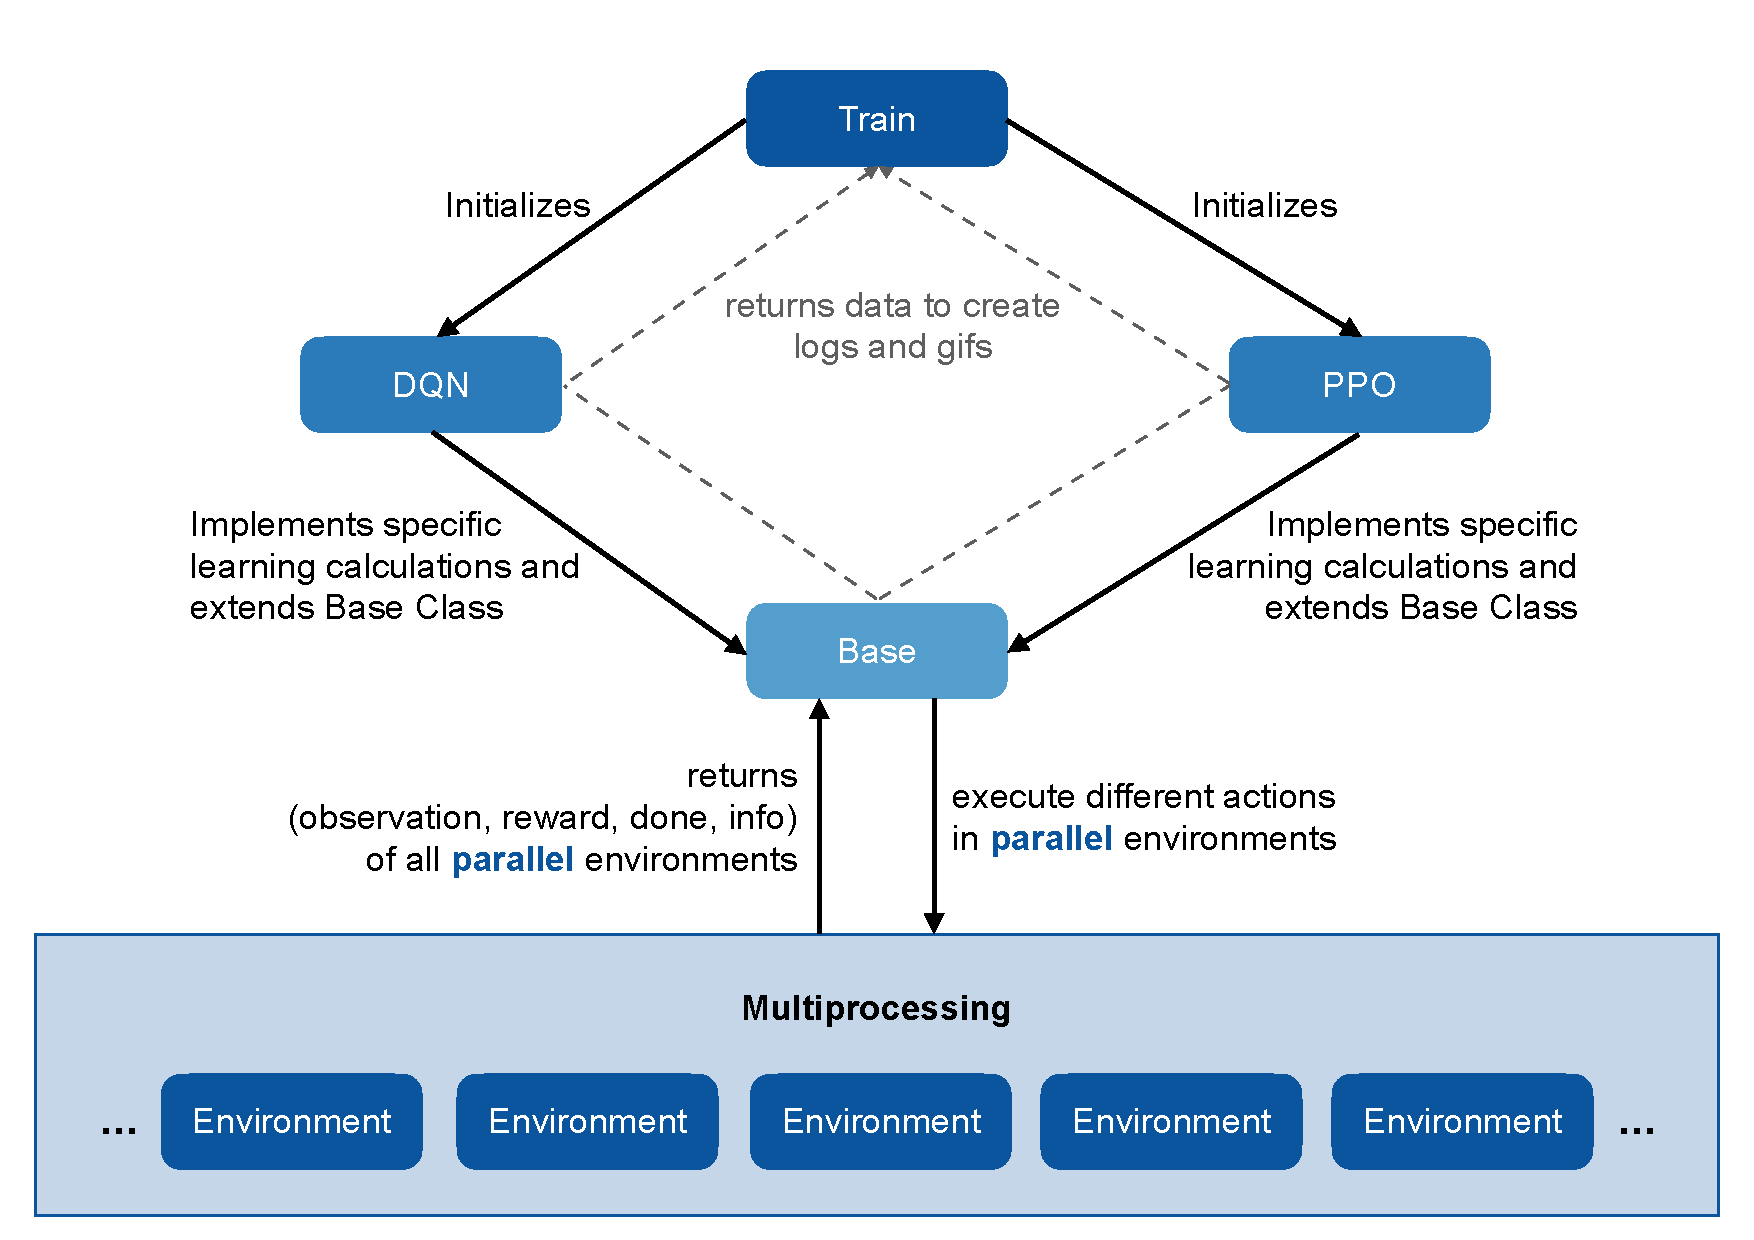
\includegraphics[width=0.9\textwidth]{pictures/training}\\
    \caption[The Training Structure]{The training structure}\label{fig:training}
\end{figure}

First, the training of agents begins by generating n environments based on the \verb|--procs| setting of the training command, see Appendix \ref{ax:training_params} for the parameter list. Each environment has the same configurations, for example \verb|--grid-size|, \verb|--agents| and \verb|--agent-view-size|. Second, the amount of \verb|--frames| is taken from the parameters, defining a general training loop, which ends once this number is reached or suceeded. During the loop, the defined training algorithm \verb|--algo| is executed.

Since both algorithms have similar procedures, they share the base class. In it a second iteration is triggered, that iterates over the amount set for \verb|--frames-per-procs|. During each step here, the agents execute actions in all parallel environments. Therefore, each step in the \verb|--frames-per-procs| iteration produces a frame in every environment. The action selection of the learning algorithms generate different decisions based on the state of each environment.

During the inner iteration, data like rewards, observations, actions and more are stored in base class variables that are accessible by the learning algorithms. When this iteration is done, the base variables are reset and log values of all episodes that reached the done state are returned to be logged, as shown in Figure \ref{fig:training}. The training loop keeps track of a frames counter, which sums up all frames that were produces by the parallel environments in the inner iteration. The training loop ends when the frames counter is greater or equal to \verb|--frames|. Otherwise, more experience batches are gathered.

Both learning algorithms include their own action selection methods. The PPO implementation relies on an actor-critic neural network, with an action space containing a probability distribution. In case of the DQN implementation the target network assigns Q values to actions, and agents choose one based on the maximum value with an epsilon greedy probability. In both variants the action selection results in one action for each agent and for each environment.

Unlike the PPO algorithm, in the DQN approach a quadruple of information is saved each frame into a replay memory. The four parts of the quadruple consist of the executed actions during that time step, the returned rewards and both the previous and new observation of the parallel environments. Until the frame amount of \verb|--initial-target-update| is reached, DQN agents only gather the quadruples but do not use them yet.

After exceeding the \verb|--initial-target-update|, the DQN learning starts. Each frame a batch of size \verb|--batch-size| is selected by randomly picking entries from the replay memory. Then, this batch is used to apply Q-learning updates to the experience samples, enhancing the training network. Every \verb|--target-update| amount of frames this training network is copied into the target network to enhance the action selection while keeping the algorithm stable.

The action selection itself is also improved during the training, by decreasing the $\epsilon$ gradually through $\epsilon = \epsilon_{end}+(\epsilon_{start}-\epsilon_{end})*e^{-\frac{frames}{decay}}$. This ensures exploration in the early phase. A high $\epsilon$ leads to actions that are picked at random. In the later course as the amount of frames increase, the $\epsilon$ gets smaller. In this case, the chance to select actions based on their Q values rises, which exploits the gathered experiences. Through \verb|--epsilon-start| and \verb|--epsilon-end| min and max values are set, and \verb|--epsilon-decay| defines the speed of reduction.

In the DQN implementation learning happens during the base class batch creation, whereas in the PPO algorithm the learning process is triggered after the creation of each base class experience batch. Basically, every time the inner loop finished, the gathered values are reshaped and saved into a PPO experience buffer. Additionally, the advantage values are calculated here and added to the buffer.

With that buffer the PPO model is now optimized. A small number of \verb|--epochs| are iterated and during each iteration random batch entries are selected. With those entries the entropies, values and losses are calculated. Afterwards, the calculation results are used to update the policy and network, as suggested in the code of \ref{fig:ppo_algo_code}.

\section{Market Settings}\label{market_settings}
To include a market into the training process, the \verb|--market| parameter can be set accordingly. The user has a choice to include an AM through the string ``am'' or a SM with ``sm''. In either case, the environment needs to adjust the action space, since agents now have the option to conduct market transactions.

Per default, the environment action space is discrete and only contains one element with five options: moving up, down, left, right or wait. Adding a market expands that discrete space into a multi discrete space. Hence, both markets require actions in form of arrays that contain three elements. However, they use different information in the action array slots. This and further distinctions and detailed procedures of each market are explained separately in the following.

\subsection{Shareholder Market}
A coloring environment that includes a SM constrains the first position of the action array to one of the five environment actions. The next position contains an agent index, towards which a buying offer will be made. Although, if this number is higher than the amount of agents in the game, the action intends no buying transaction. The last array position contains either a zero or a one, with one signalizing that the agent wants to sell its share. An abstract representation of a shareholder action array is: \verb|[environment_action, agent_index, sell_share]|.

\begin{figure}[hpbt]
    \centering
    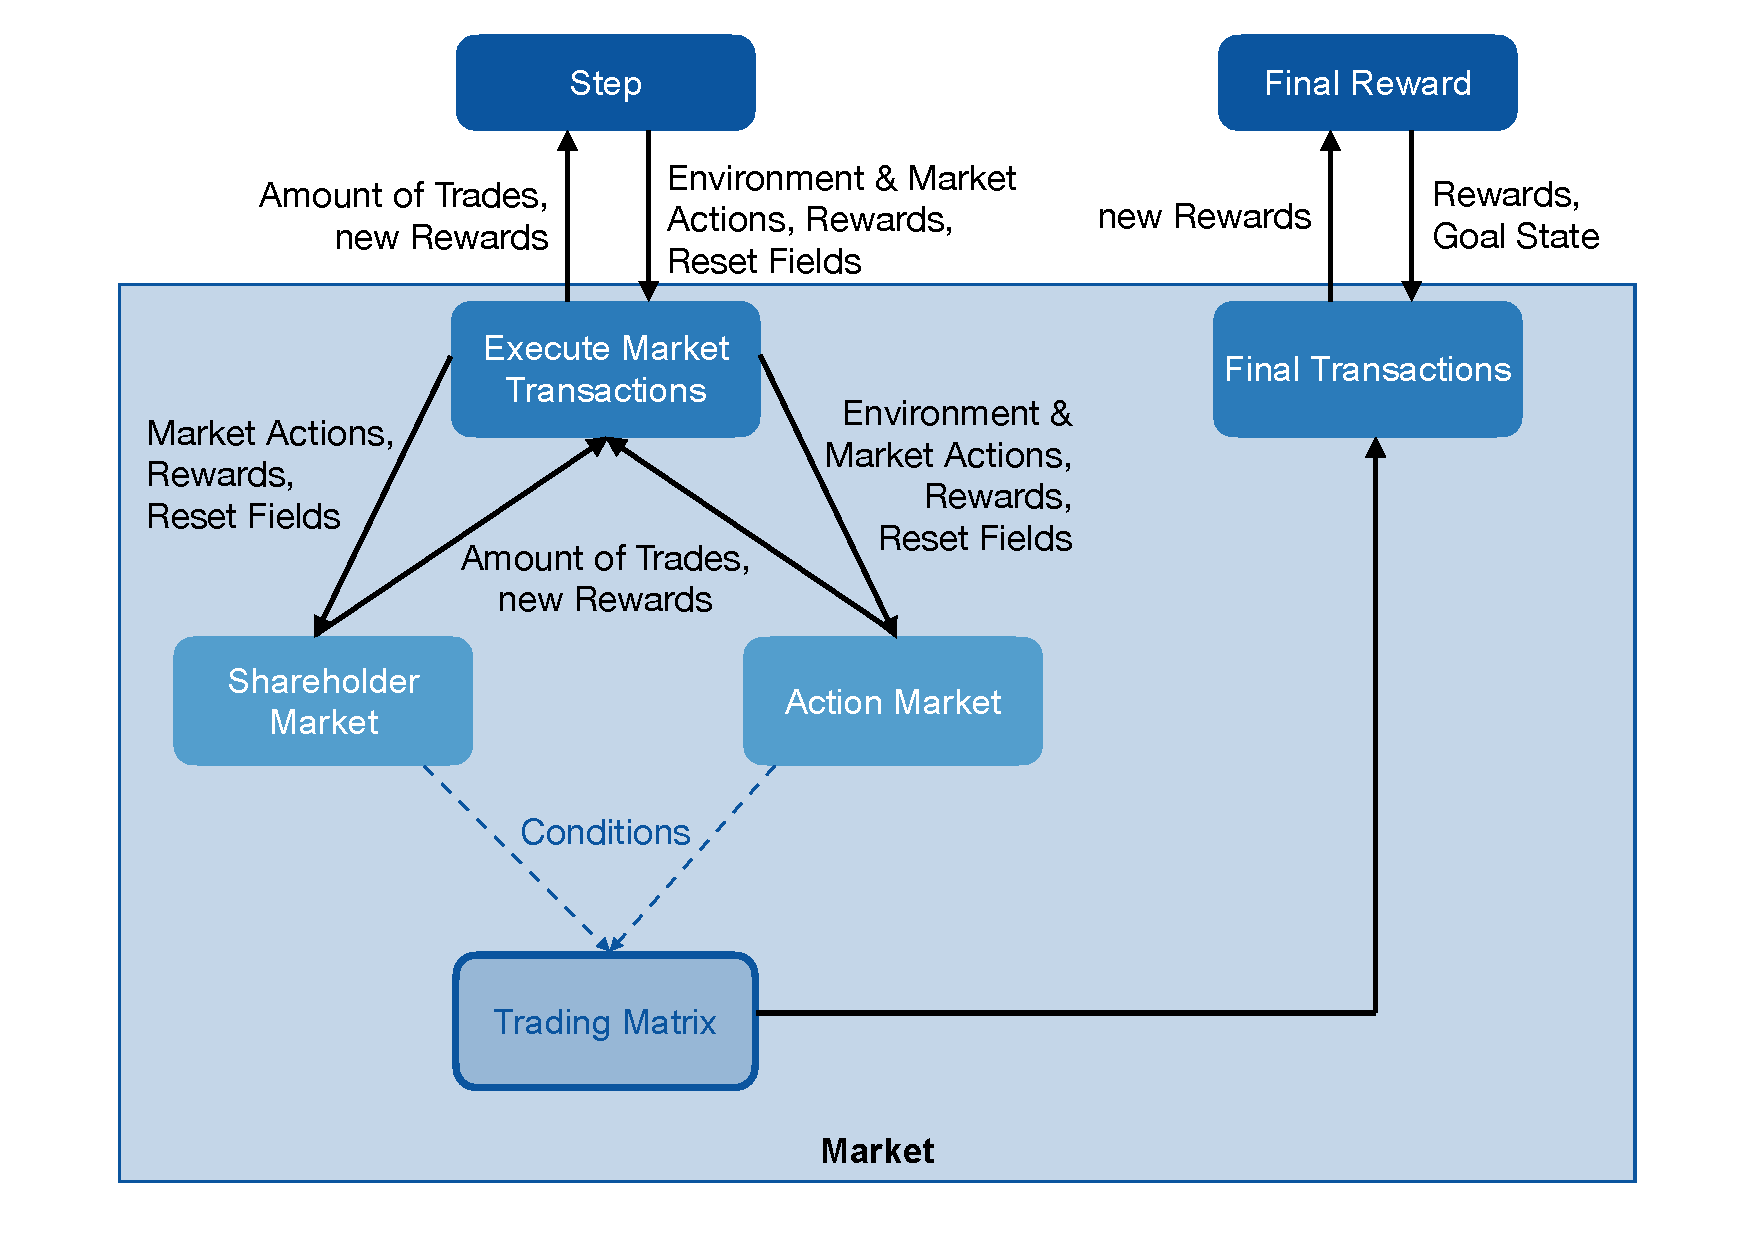
\includegraphics[width=0.9\textwidth]{pictures/market}\\
    \caption[Market Elements]{The market elements}\label{fig:market}
\end{figure}

In Figure \ref{fig:market} market elements are visualized. On the left, the process that takes place during each step is shown, see algorithm \ref{algo:step_reward} line 10. Here, the market always receives an action array that is already divided in two parts, one part only containing the first array position and the other part includes the buying and selling information in this case.
% Since transactions alter the rewards, the current reward is also transmitted. Lastly, an array of agent indices that have recently reset cells is also given, since some transaction conditions make use of that information.

In the course of the market calculations a trading matrix is altered. This matrix is quadratic with dimensions equal to the amount of agents. In a shareholder trading matrix, the diagonal contains ones, since every agent starts with the full ownership over their own shares. All other matrix slots are filled with zeros. An example for an initial trading matrix is shown below.
\begin{equation*}
trading\_matrix = 
\begin{pmatrix}
1 & 0 \\
0 & 1
\end{pmatrix}
\end{equation*}

The first thing to check in a market step execution is the market type. The type can be set with the \verb|--market| parameter and the market receives this setting during initialization. If the market type includes the string ``sm'' the SM matches and the corresponding function is called. 
% In this case the environment actions are not of importance, so the function receives all other parameters instead. 
Inside the shareholder function two additional matrices are created in each step, a buying matrix and a selling matrix. Both matrices are always initially filled with zeros, are quadratic, and their dimensions is equal to the amount of agents, similar to the trading matrix. Depending on the market action the buying matrix is altered to contain a one in the row of the buyer and the column of the agent that the offer is directed to.
% Here, the diagonal stays zero, since agents are prohibited of buying from themselves. 
Each agent can only buy one share at a time, therefore here the rows contain at maximum one entry. The same applies to the selling matrix, which contain ones on the diagonal for the agent that wants to sell according to the market actions.

After setting up and filling out the two matrices they are iterated, extracting the rows entries of each matrix and defining the corresponding indices as buyer and seller. A transaction takes place if the following conditions are met:
\begin{itemize}
    \item the buyer is not equal to the seller
    \item all entries of the buyer row and the seller row match
    \item the sellers shares are greater than the \verb|--trading-fee|
\end{itemize}

If all conditions are true, the trading matrix is updated here, by changing the share of the selling agent, adding the subtracted amount to the buyer. The amount can be set with \verb|--trading-fee|, which is 0.1 per default. The last condition ensures, that agents still receive some of their own rewards and do not trade everything off. 

An example for a transaction could be two agents acting in an environment. If agent two buys a share from agent one, the trading matrix is updated. The second row stores the shares of agent two, which increases by 0.1 on the first position. This signalizes that agent two is owner of some shares of agent one and still has 100\% of its own shares. In response, the shares in the first row and column of agent one decreases to 0.9.
\begin{equation*}
trading\_matrix = 
\begin{pmatrix}
1 & 0 \\
0 & 1
\end{pmatrix} \xrightarrow[\text{from Agent 1}]{\text{Agent 2 buys}} 
trading\_matrix = 
\begin{pmatrix}
0.9 & 0 \\
0.1 & 1
\end{pmatrix} 
\end{equation*}

Additionally, the rewards of the current step calculation, would be updated here, if a price for the shares are set. In this implementation however, the shares have no price since agents are willing to give them away for free. Otherwise, the price would be subtracted from the buying agents' reward and that value would be added to the reward of the selling agent. 

In any case, the SM triggers a reward calculation according to the trading matrix in every step. This means, that for the example above, agent two will receive 10\% of the rewards from agent one in every step, until the episode ends. However, this is only the case in the steps in which agent one is not in dept.

Further details of the reward calculations in markets will be discussed in Section \ref{market_reward_calc}. Lastly, the transaction count is documented for evaluation purposes. At this point the market execution for the current step is done and the number of executed trades and the updated rewards are returned to algorithm \ref{algo:step_reward}.

\subsection{Action Market}
The agent action shape of an AM environment is similar to the shareholder action array. Again, an action has three slots, with the first being the environment execution and the second being the index of an agent a buying offer is directed to. The difference to a shareholder action is the last array position. Instead of setting a bit here to signalize the willingness of selling shares, the agent chooses an environment action that is expected from the agent of position two. Hence, an abstract representation of an action in the AM is the following: \verb|[environment_action, agent_index, expected_action]|.

The market elements and general process of visualization \ref{fig:market} also apply to an AM setting. Here however, the trading matrix is initially filled with zeros. 
% Furthermore, the AM function needs all parameters, including the environment actions. This information is crucial to the transaction conditions, which are:
To establish a transaction the market actions are examined, and the following conditions checked:
\begin{itemize}
    \item the buyer differs from the receiving agent
    \item the environment action of the receiving agent matches the expected action
\end{itemize}

When the two conditions apply a market transaction takes place. The \verb|--trading-fee| parameter decides the price the buyer pays the receiving agent. Both the rewards and trading matrix are altered here, by subtracting the price from the buyer and adding it to the receiver. An example of the trading matrix update in this market setup is shown below. Here again agent two is purchasing from agent one.
\begin{equation*}
trading\_matrix = 
\begin{pmatrix}
0 & 0 \\
0 & 0
\end{pmatrix} \xrightarrow[\text{from Agent 1}]{\text{Agent 2 buys}} 
trading\_matrix = 
\begin{pmatrix}
0 & 0.1 \\
0 & -0.1
\end{pmatrix} 
\end{equation*}

The trading matrix stores the market balance of both agents in each row. For agent two this means that the negative value was spent. The first row shows that agent one still has a neutral balance and gained the \verb|--trading-fee| of 0.1 from agent two. To conclude, the market returns the number of transactions that took place in this step and the new rewards.

\subsection{Reward Calculations}\label{market_reward_calc}
During each step agents can update the trading matrix by acting on the market. With each update the rewards are also changed. In Figure \ref{fig:market_rewards} a detailed example of the reward update in a market is shown. It is worth mentioning that it is not possible to execute both markets simultaneously, but rather one or none must be set for a training process. This illustration shows both calculations in one image for convenience. Equal to the previous examples, the red agent two buys a share or action from the blue agent one. For both market scenarios the \verb|--trading-fee| is set to the default value and both agent rewards start at 0.1. On the top half of the image the internal market calculation of a SM is shown, and the bottom half illustrates the calculation of an AM.
\begin{figure}[hpbt]
    \centering
    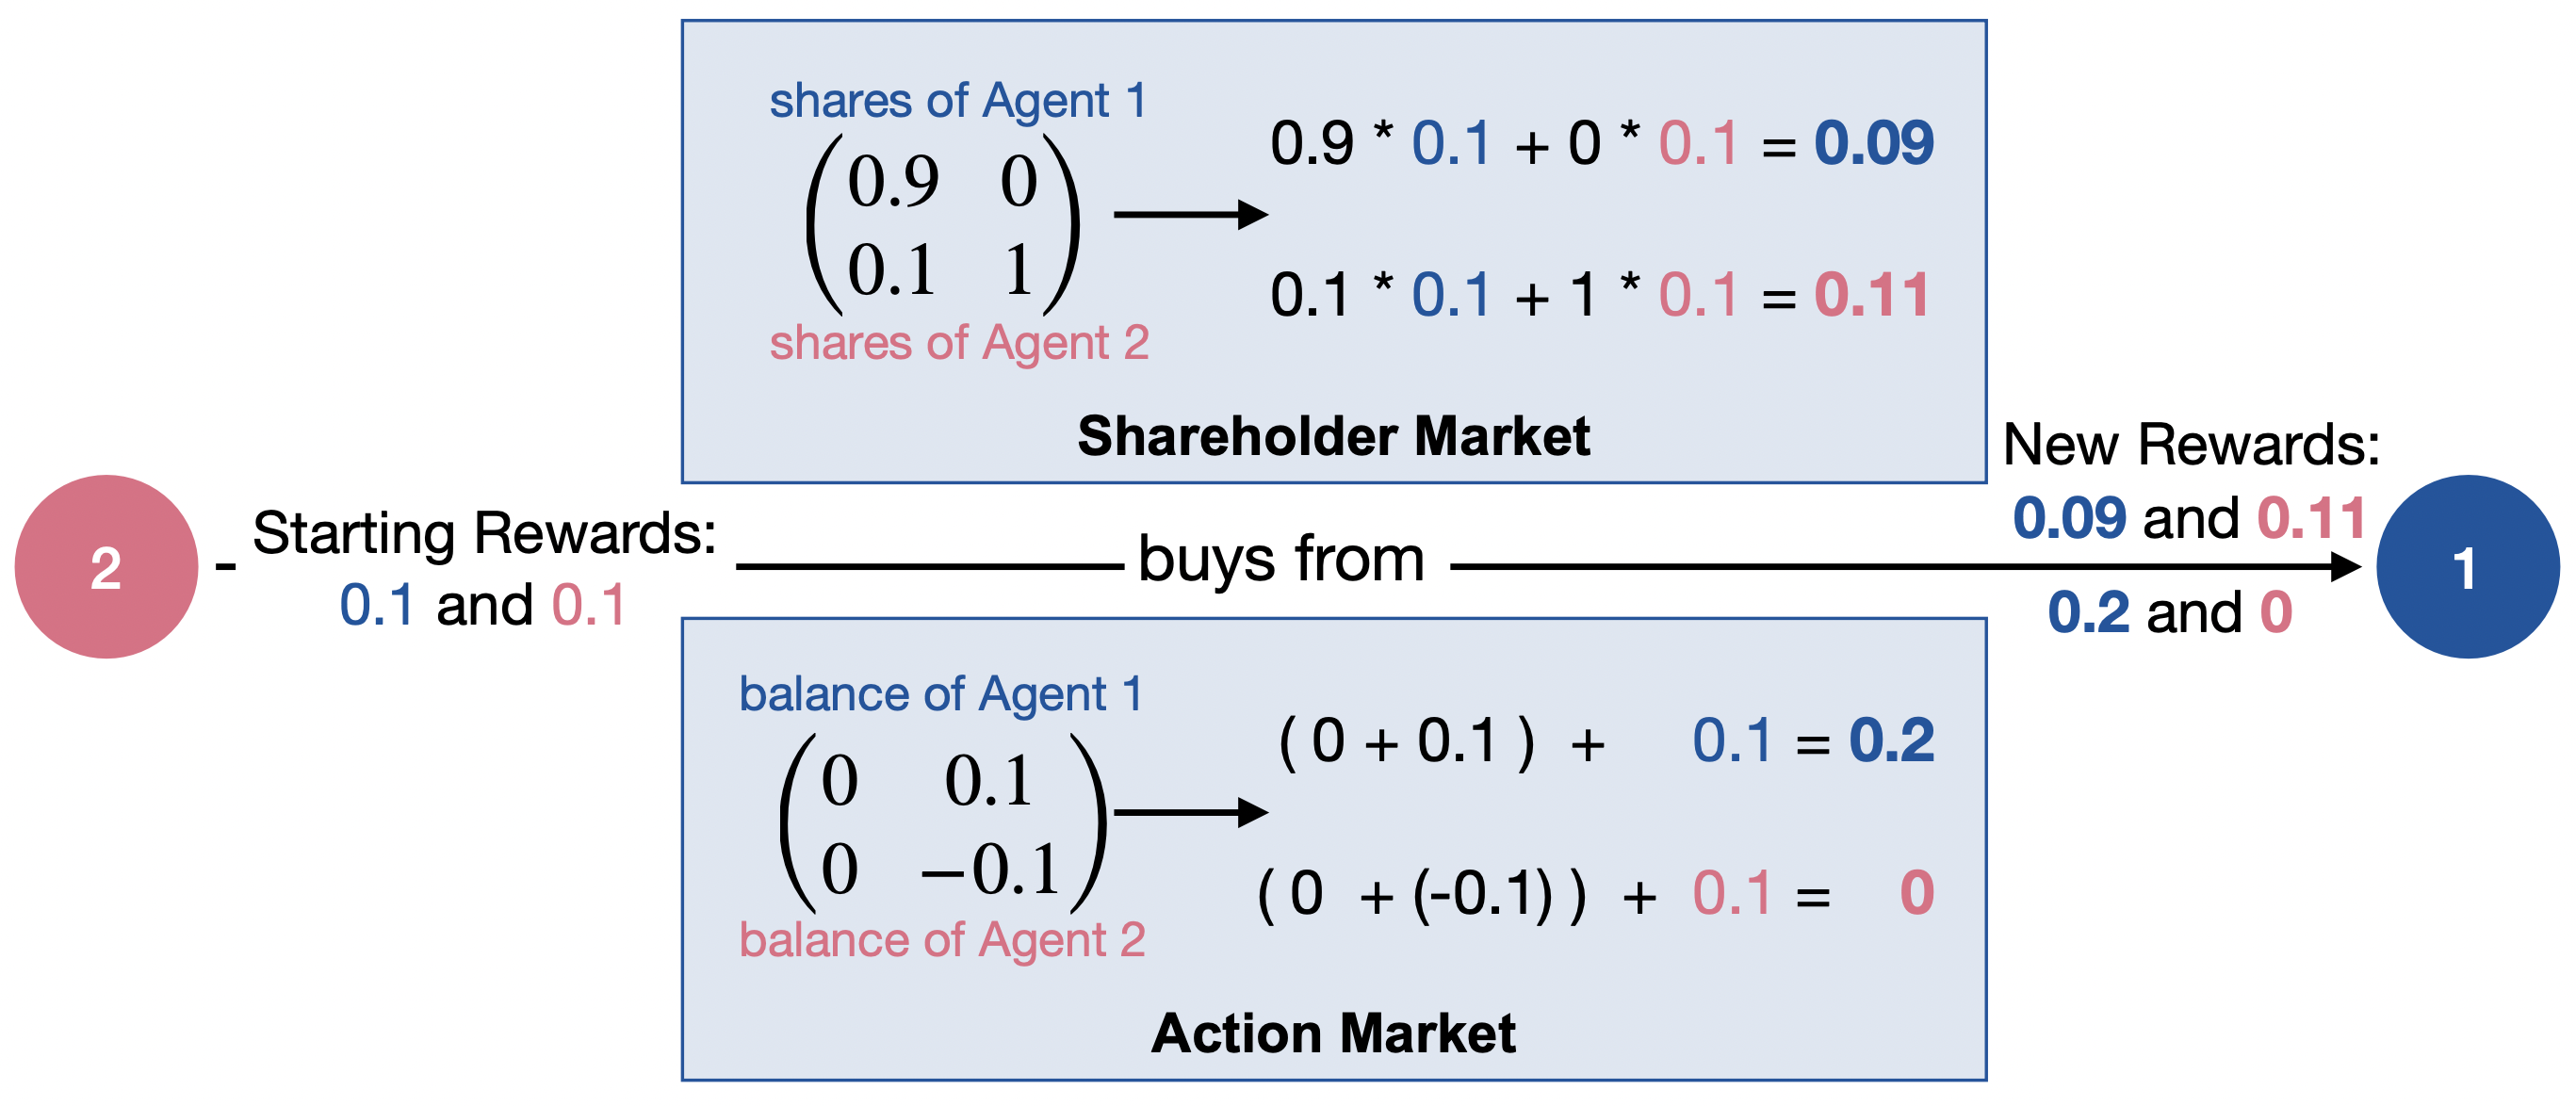
\includegraphics[width=0.9\textwidth]{pictures/new_market_rewards}\\
    \caption[Exemplary Reward Calculation Of Markets]{Exemplary reward calculations of both market types}\label{fig:market_rewards}
\end{figure}

In a SM the trading matrix represents the distribution of agent shares. Each matrix column adds up to one, representing a 100\% share of an agent. As mentioned earlier the diagonal of the matrix is initially set to one since agents start with complete ownership over their shares. For this example the trading matrices are configured accordingly. The first matrix row implies that agent one is owner of 90\% of its own shares and is not owner of any shares from agent two. Whereas the second row shows that agent two claims 10\% of the shares of agent one and has full ownership over its own.

To generate the new rewards of the agents, the market multiplies all current rewards with each matrix rows. The resulting products of each row are then summed up to represent the new reward of the corresponding agent. For the example, agent one gets a new reward value of 0.09 and agent two claims 0.01 from agent one and adds that to its full value of 0.1, resulting in a new reward of 0.11. 

In contrast to an AM in a SM the rewards are just reassigned based on the current shares of the trading matrix. An exception occurs, when agents have negative rewards. In this case their share will be skipped during the redistribution, since shares are used to participate in profits. 

Another difference to AMs is that the shown SM reward redistributions are executed in each step, and it is irrelevant whether market actions were executed. The only exception however is the last step, when the done flag is set to true. In this case the final rewards, see algorithm \ref{algo:final_reward}, need to be calculated first, before the shares are taken into account.

AMs, in most cases, update the rewards directly and only once, when a transaction is executed. The trading fee is immediately subtracted from one agents' reward and added to the counterpart during the trade. If an agent can not afford the fee the process is completed anyway and the agent goes into debt. 

Thus, this market type makes no use of the trading matrix. Nonetheless, the matrix is always updated, since a specific scenario requires the calculations to be executed at the end, see Section \ref{market_conditions}. In this case, the agents market balance, stored in the matrix rows, is summed up and added to the current reward. This procedure is illustrated in the bottom half of figure \ref{market_reward_calc}. Here, the fee of 0.1 is subtracted from agent two and added to the reward of agent one, leading to new rewards of 0.2 for agent one and zero for agent two.

\subsection{Additional Conditions}\label{market_conditions}
The \verb|--market| string for both types can be extended to add more conditions, namely with ``no-reset'', ``no-debt'' and ``goal''. The ``no-reset'' string enables the check whether the buyer has recently reset a cell. If that is the case, the corresponding buyers are ignored on the market for the current step. Hence, their market actions will not be applied. However, in a SM the penalized agent can still sell its shares. 

With the ``no-debt'' Flag, transactions only take place if buyers can afford to pay the price. In this implementation with AMs and the default fee, this is solely the case if agents have colored a cell in that step. Waiting or misbehaving agents are excluded as buyers, since their rewards result in 0 or -0.1, which does not meet the fee of 0.1. For SMs this depends on the presence of a share price. Per default the price is zero, similar to the approach of Schmid et al. \cite{scbe21}, making this condition irrelevant for the SM setting.
% TODO kommt zu goal Both market conditions can be used simultaneously.

The last addition, ``goal'', lets the market process run as usual, only removing the reward changes during the steps. Here, all transactions are just documented into the trading matrix during an episode. Eventually, the transactions are executed once the final rewards of algorithm \ref{algo:final_reward} is calculated. As shown on the right side of Figure \ref{fig:market}, the market obtains those rewards and a Boolean describing whether the environment goal was reached.

The rewards are updated with the trading matrix content when either of the two conditions is satisfied:
\begin{itemize}
    \item ``goal'' addition is present and environment goal was reached
    \item no ``goal'' addition and market type is a SM
\end{itemize}
Otherwise the rewards are return as they are and will not be processed further. 

For such goal oriented markets, regardless of the type, the final environment state needs to equal the overall aim. Thus, the whole grid has to be colored, to execute the final market transactions.

% Since the goods of a SM are shares, naturally the current reward values are of importance. During the step calculations of the rewards the done flag is  takes place at the end of an episode. In an AM however, each step is self-contained in regards to transactions and payouts. Nonetheless, with the ``goal'' addition, the payout also shifts to the end of episodes. 

If the first condition applies and an AM is present the rewards are updated by using the trading matrix. For a SM either condition must be met in order to generate the final reward. The calculations for both cases are equal to the example of Chapter \ref{market_reward_calc}.
% Again, the trading matrix rows and rewards are iterated here. Each row element is multiplied with the reward of the same index and added to the new reward of that agent. An example of both operations is shown in Figure \ref{fig:market_rewards}.

After the final market updates to the rewards the new values are returned, as shown in Figure \ref{fig:market}. The last thing to point out is that the additional market conditions can be used in combination, making ``sm-goal-no-reset-no-debt'' for example a valid \verb|--market| setting.
% % -------------------------------------------------------------------------------------------------
%      MDSG Latex Framework
%      ============================================================================================
%      File:                  introduction-[UTF8,ISO8859-1].tex
%      Author(s):             Michael Duerr
%      Version:               1
%      Creation Date:         30. Mai 2010
%      Creation Date:         30. Mai 2010
%
%      Notes:                 - Example chapter
% -------------------------------------------------------------------------------------------------
%
\chapter{Implementation}\label{sec:Implementation}
- How exactly did you do it? \\
- Experiment parameters \\
- Experiment setup \\
- No need to mention framework, software libraries or tools

\section{Learning Algorithms}
PPO, DQN -> OBSERVATION VALUE and how network receives and processes it into!

Independent learning! each agent has own actor/critic or complete network

\section{Agent Compositions}
env setting: coop vs mixed vs mixed competitive and how the Gridwold/reward calculation behaves

\section{Reward Calculations}
normal/percentage based and market
% -------------------------------------------------------------------------------------------------
%      MDSG Latex Framework
%      ============================================================================================
%      File:                  introduction-[UTF8,ISO8859-1].tex
%      Author(s):             Michael Duerr
%      Version:               1
%      Creation Date:         30. Mai 2010
%      Creation Date:         30. Mai 2010
%
%      Notes:                 - Example chapter
% -------------------------------------------------------------------------------------------------
%
\chapter{Results}\label{sec:Results}
% - Result presentation
% - Description of images and charts \\
% - One Agent Environment vs MARL
% - Best cases of reward, trades, grid coloration, field resets
% - Worst cases of above
% - influence of markets
In this chapter the results of various training executions with different parameters are compared. All possible combinations of markets, agent compositions and learning algorithms in an easy environment are shown in section \ref{easy_env}. The best combinations are then extracted and applied in more challenging environment setups, which are compared in section \ref{difficult_env}. 

\section{Easy Environment Setup} \label{easy_env}
\marginpar{was wurde untersucht}
The results of this research compare multiagent trainings with varying settings, namely acting in different compositions and markets. In this case the amount of agents stays fixed and is greater than one. The agents use either of the two learning approaches PPO or DQN to train. Hence, the overall possible comparisons include a total amount of 102 executions. This number results from the calculation of multiplying the 2 learning algorithms with the 3 possible agent compositions (cooperative, competitive and mixed-motive) and additionally 2 optional markets that can contain 3 modular additions. 

The market options are for example the following SM instances: 
\begin{itemize}
    \item ``sm''
    \item ``sm-goal''
    \item ``sm-no-debt''
    \item ``sm-no-reset''
    \item ``sm-no-reset-no-debt''
    \item ``sm-goal-no-debt''
    \item ``sm-goal-no-reset''
    \item ``sm-goal-no-reset-no-debt''
\end{itemize}
The 8 options above are also applied on the AM and lastly the option of no market needs to be considered, leading to 17 market scenarios. Calculating the total amount of executions now by using those 17 market possibilities results in the 102 executions.

\marginpar{was wurde nicht untersucht}
Yet, not all market arrangements are needed. For example, the mix of ``no-reset'' and ``no-debt'' is not of use in this implementation. An agent that has reset a field has a reward of -0.1 and therefore already is in debt, which means that ``no-debt'' includes ``no-reset''. This subtracts 4 compositions from the 17 market scenarios. Additionally, shares are free of charge, making the options ``sm-no-debt'' and ``sm-goal-no-debt'' irrelevant. Agents can always afford to buy shares in this case. The SM is therefore left with 4 combinations and the overall market scenario count is now 11. In total the analyzation only includes 66 training results. 

\marginpar{wie wurde untersucht / zahlen}
In order to compare the market approach with a credit assignment solution in the cooperation composition, the training with a DR setting is also included. This in turn adds another execution to each learning algorithm. Furthermore, to ensure that the environment is generally solvable, one agent first trains in the environment setup with each learning algorithm using similar hyperparameter as in the multiagent case. To summarize the execution count is therefore 70 in total.

Those 70 executions are mostly run with the default parameters that can be looked up in Appendix \ref{ax:training_params}. The agents solve an empty 5 by 5 grid, in which they can only walk inside a 3 by 3 field, due to the surrounding walls, see Figure \ref{fig:1-easy}. The maximum amount of steps the agents are allowed to take is set to 25, if not specified otherwise. This count is generated by squaring the grid size.

Overall the training with default parameters expands over 80.000 frames, of which every 128 (\verb|--frames-per-proc|) are processed in each of the parallel environments. In this case the amount of parallel environments is set to 16 with the parameter \verb|--procs|. All the data that is returned by the environments is saved in one entry. Most of the time the data is summarized into mean values or occurrences are counted. Furthermore, the data entries are always 2048 frames apart, since all 16 environments process 128 actions before a new data entry is logged. After saving each entry the variables containing mean values or counters are reset to produce new values in the next frames. \\\\

% Those data entries 2048 frames are referred to as a batch. After each data batch, mean values and counters of all finished episodes are calculated and logged, for example mean rewards, mean grid coloration, amount of goal states or reset fields etc... 
% In the worst case scenario, where the episode always ended because the 25 default steps were used up, the data entry would contain values of 80 episodes. This is result of 25 fully executed steps in a span of 128 frames, leading to 5 finished episodes. This is the case for each of the 16 parallel environments. Afterwards, After each entry, all log variables are cleared to produce new values in the next frames. All environment data are put together to either calculate mean values or count occurrences.

% ------------ ONE AGENT RESULTS ----------------
\begin{minipage}{\textwidth}
  \begin{minipage}[b]{0.29\textwidth}
    \centering
    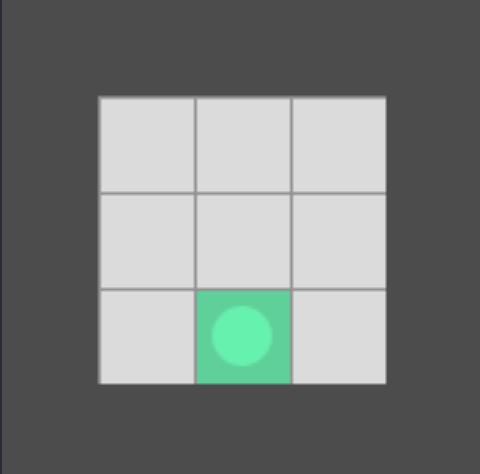
\includegraphics[width=1\linewidth]{1-agent-easy.png}\\
    \captionof{figure}[One Agent Level Easy]{Visualization of level easy with one agent}\label{fig:1-easy}
  \end{minipage}
  \hfill
  \begin{minipage}[b]{0.69\textwidth}
    \centering
    \begin{tabular}{lc}\hline
      Setting & Fully colored \\ \hline
        1 ppo & 2130 \\
        1 dqn & 650 \\ \hline
      \end{tabular}
      \captionof{table}[Training Results for one Agent Level Easy]{Number of times the agent fully colored the environment during training with each learning algorithm.}\label{t:1-easy}
    \end{minipage}
  \end{minipage}\\\\

Table \ref{t:1-easy} shows the amount of times the grid on the left (Figure \ref{fig:1-easy}) was fully colored by one agent using each training algorithm. It is important to mention here, that the maximum step amount is set to 10 in both cases. Additionally, this and all following dqn executions have a \verb|--batch-size| set to 64 instead of the default 256. The ppo agent colored the whole grid a total amount of 2130 times and the dqn agent 650 times.

\begin{figure}[hpbt]
    \centering
    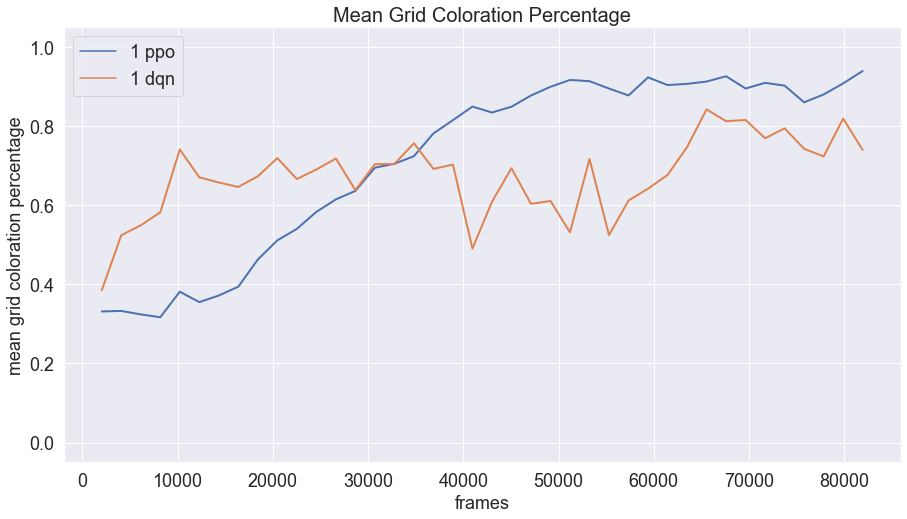
\includegraphics[width=0.8\textwidth]{1-easy-plot.png}\\
    \caption[Mean Grid Coloration Percentage of one Agent]{The mean coloration percentage of a 5x5 grid and one acting agent}\label{fig:1-easy-plot}
\end{figure}

The average grid coloration percentage of those settings is shown in plot \ref{fig:1-easy-plot}. The plot lines start at around 2048 frames, since this marks the first time a data entry of the parallel environments is returned. Furthermore, the plot exceeds the 80.000 default \verb|--frames|, since the last data entry includes the last data batch of the environments. The table shows, that both training runs solve the environment and the plot illustrates that in both cases generally a high percentage of the grid is colored. The dqn execution yields a better performance in the early stage, whereas the ppo agent gradually improves over time. In both cases an average coloration of over 70\% is eventually reached. 

Now the multiagent scenario is compared. Here a set of two agents are trained to color the field of the same default dimensions, see Figure \ref{fig:2-coop-easy}. However, every agent executes an action during a step and with 10 steps and two agents in theory 20 cells could be visited. Hence, the \verb|--max-steps| count is reduced to 8. 

In order to get an overview of the overall 70 training results, the remaining 68 multiagent executions are divided into three different \verb|--setting| values. The first data division only covers the cooperation compositions, including ``difference-reward''. Table \ref{t:2-coop-easy} illustrates the scoreboard of the top three executions in this specification for each learning algorithm. \\\\

% ------------ COOP RESULTS ----------------
\begin{minipage}{\textwidth}
  \begin{minipage}[b]{0.29\textwidth}
    \centering
    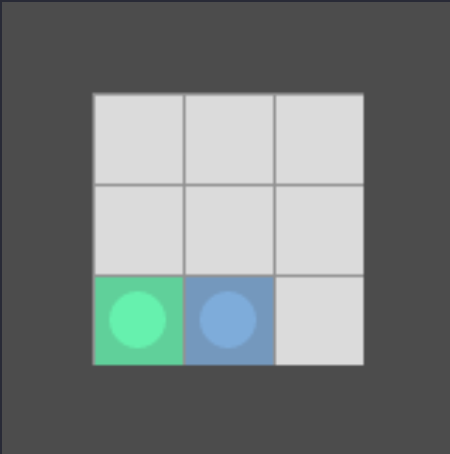
\includegraphics[width=1\linewidth]{2-agents-easy.png}\\
    \captionof{figure}[Two Agents Level Easy]{Visualization of level easy with two agents}\label{fig:2-coop-easy}
  \end{minipage}
  \hfill
    \begin{minipage}[b]{0.69\textwidth}
    \centering
    \begin{tabular}{lc}\hline
        Top 3 PPO Cooperation Settings & Fully colored \\ \hline
        2 ppo difference-reward & 889 \\
        2 ppo & 125 \\
        2 ppo sm-goal & 32 \\ \hline
         &   \\ \hline
        Top 3 DQN Cooperation Settings & Fully colored \\ \hline
        2 dqn difference-reward & 5949 \\
        2 dqn am-goal-no-debt & 3197 \\
        2 dqn am-goal & 2880 \\ \hline
        \end{tabular}
        \captionof{table}[Training Results for two Cooperation Agents Level Easy]{Number of times two agents working in cooperation fully colored the environment during training.}\label{t:2-coop-easy}
    \end{minipage}
  \end{minipage}\\\\

The measured attribute here is again the overall amount of fully colored states. In both cases the agents with the DR setting scored best, 889 times with the DQN algorithm and 5949 times by using PPO. The PPO scores continue with the default cooperation scenario on second and the SM with the goal condition on third place. 

On the contrary, the DQN results show AM settings on the remaining places, with the additions ``goal-no-reset'' on second place and ``goal'' on the third place. It is visible, that in both scoreboards the second and third executions are far behind the corresponding DR setting in terms of fully coloration counts.

\begin{figure}[hpbt]
    \centering
    %%----start of first subfigure----
    \subfloat[Reward summary of PPO agents]{
        \label{fig:2-ppo-coop-easy} %% label for first subfigure
        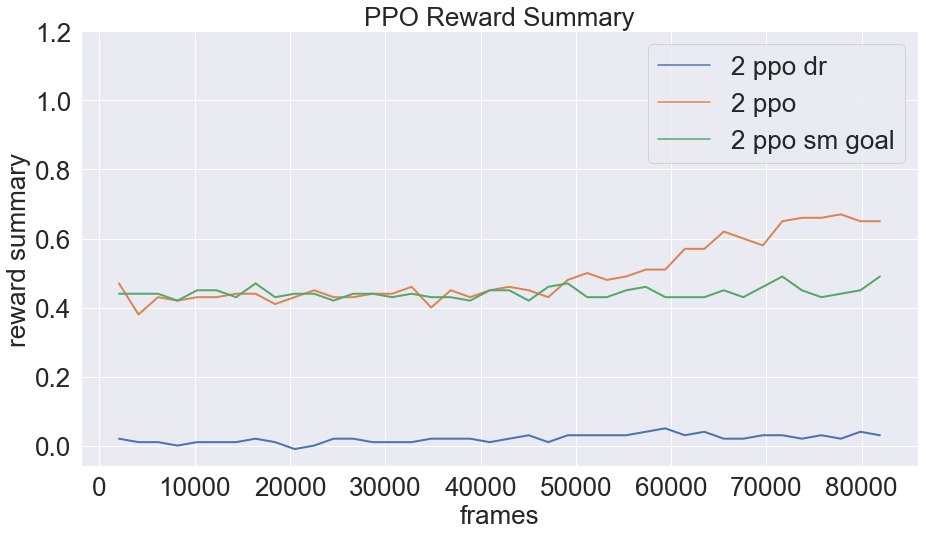
\includegraphics[width=0.48\linewidth]{2-ppo-easy.png}}
    \hspace{0.01\textwidth}
    %%----start of second subfigure----
    \subfloat[Reward summary of DQN agents]{
        \label{fig:2-dqn-coop-easy} %% label for second subfigure
        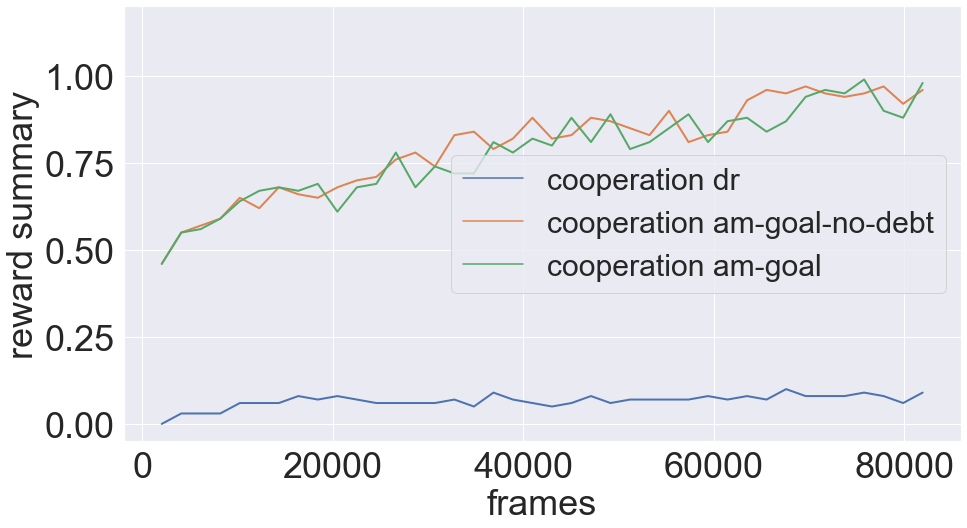
\includegraphics[width=0.48\linewidth]{2-dqn-easy.png}}
    \caption[Reward Summaries of the Top Cooperation Modes]{Reward Summaries of the top three cooperation compositions using PPO (left) and DQN (right)}
    \label{fig:multipic_plots_coop_easy} %% label for entire figure
\end{figure}

In the two plots of Figure \ref{fig:multipic_plots_coop_easy} the reward summary of the top scores, see table \ref{t:2-coop-easy}, are displayed. The term reward summary is used here, since the rewards of cooperating agents are equal and sometimes contain only slight changes through markets. However, in other agent compositions the rewards are rather specific to each agents' contribution. In any case the logged training data contains the mean reward of every agent separately. 

In order to summarize cooperation rewards, the average value of those separate agent rewards is calculated for each data entry and the results are then plotted here. For reward summaries of all other compositions each data entry is summarized with the sum of the separate agent rewards. The maximum y-axis label here is set to 1.2, since agents can get a reward of 1.1 if they color the whole field and additionally get a reward of 0.1 for the final step. Through the reward summary calculations rounding errors may occur, which could in turn exceed the maximum reward of 1.1. Furthermore, markets could also contribute to bigger rewards. 

Even thought, the executions with the DR configuration scored highest in terms of reaching the goal, the reward line in this case stays around 0.1. The reason for that is, that agents get the difference of two rewards, leading to very small values. The rewards of the dqn executions show a continuous increase and almost exceed an average summary reward of 1. On the contrary, the ppo executions, excluding the DR setting, only show a small reward increase at the last third half of the training. The DR execution shows now striking changes here.

The next training executions to look at are ``mixed-motive'' settings. Here again a scoreboard, listing the top three results of each learning algorithm, is shown in table \ref{t:2-mixed-easy}.
% ------------ MIXED RESULTS ----------------
\begin{center}
    \begin{tabular}{lc}\hline
        Top 3 PPO Mixed-Motive Settings & Fully colored \\ \hline
        2 ppo mixed-motive & 1006 \\
        2 ppo mixed-motive sm-no-reset & 764 \\
        2 ppo mixed-motive sm & 680 \\ \hline
         &   \\ \hline
        Top 3 DQN Mixed-Motive Settings & Fully colored \\ \hline
        2 dqn mixed-motive sm & 5417 \\
        2 dqn mixed-motive am-no-reset & 5379 \\
        2 dqn mixed-motive sm-goal & 5302 \\ \hline
        \end{tabular}
        \captionof{table}[Training Results for two Mixed-Motive Agents Level Easy]{Number of times two agents working in a mixed-motive setting fully colored the environment during training.}\label{t:2-mixed-easy}
    \end{center}

While the default SM configuration occupies the first place of the DQN scoreboard, in the PPO board it is only on the third place. In fact, the first place of the ppo training is the plain ``mixed-motive'' setting without any additions. On the second place here is a SM training with the ``no-reset'' condition. The fully colored counts are very similar between the PPO trainings. The same applies to the values of the DQN board. The second place here is also occupied by a ``no-reset'' addition, however in this case it is applied to an AM. On the third place of the DQN executions is a SM with the ``goal'' addition.


% ------------ COMP RESULTS ----------------
\begin{center}
    \begin{tabular}{lc}\hline
        Top 3 PPO Competitive Settings & Fully colored \\ \hline
        2 ppo competitive & 3178 \\
        2 ppo competitive sm-no-reset & 2645 \\
        2 ppo competitive sm & 2437 \\ \hline
         &   \\ \hline
        Top 3 DQN Competitive Settings & Fully colored \\ \hline
        2 dqn competitive sm-goal-no-reset & 7877 \\
        2 dqn competitive sm & 7842 \\
        2 dqn competitive am-goal-no-debt & 7560 \\ \hline
        \end{tabular}
        \captionof{table}[Training Results for two Competitive Agents Level Easy]{Number of times two agents working in a competitive setting fully colored the environment during training.}\label{t:2-comp-easy}
    \end{center}


\section{Difficult Environment Setup} \label{difficult_env}
% -------------------------------------------------------------------------------------------------
%      MDSG Latex Framework
%      ============================================================================================
%      File:                  introduction-[UTF8,ISO8859-1].tex
%      Author(s):             Michael Duerr
%      Version:               1
%      Creation Date:         30. Mai 2010
%      Creation Date:         30. Mai 2010
%
%      Notes:                 - Example chapter
% -------------------------------------------------------------------------------------------------
%
\chapter{Discussion}\label{sec:Discussion}
- Are the findings as expected? \\
- Why are the things as they were observed? \\
- New experiments that provide further insights \\
- Make your results more comprehensible
\chapter{Conclusion}\label{sec:Conclusion}
Each of the three compositions presented in chapter \ref{env} lead to learning problems or game losses. Cooperation may reward misbehavior, namely field resetting, resulting in the CAP of chapter \ref{CAP}. In mixed-motive or fully competitive settings, the overall goal may never be reached, due to greediness or disorder. This research compared the effects of markets not only on mixed-motive settings as suggested by Schmid et al. \cite{scbe21}, but on all three agent compositions.

During the thesis, the coloring environment was presented. It enables agents to color cells by moving around. Stepping on colored cells removes the color and penalizes the agent, coloring cells rewards them. In competitive agent compositions, agents can take over cells and do not reset them. The goal was to color the whole grid in order to get the highest reward. The thesis aims to compare the effect of markets in the three agent compositions and whether SMs or AMs could solve the problems multiagent environments face.

Overall, the CAP does not seem to be solvable through markets applied in the coloring environment. The performance of the DR executions could not be met by any market type. Increasing the grid size and amount of agents also showed that cooperative settings with markets failed to reach the goal completely. This could be an indicator for agents struggling to understand how their actions contributed to the observations and shared rewards. In the mixed-motive and competitive compositions, trainings with markets achieved fully colored grids, even in the difficult setup. This shows an alignment and organization between the agents. Nonetheless, in the most challenging environment, a nine by nine room divided grid, none of the compared settings helped the agents learn how to solve the task.

All in all, one could argue, that the parameters need some adjustments for the different challenges to achieve better results. For instance, reducing the fee in AMs and increasing it for SMs, and generally fine-tuning the hyperparameters of the learning algorithms for each setup. Another point is to conduct all 70 training executions in all challenges, rather than filtering the best settings through the results of an easy training setup. It would also be interesting to compare the results of agents, who always have the full view of the environment with this partially observable implementation.

The coloring environment also leaves room for expansions. More environment shapes could be defined, instead of just a quadratic instance. It would be interesting to see how different reward values for good or bad actions might affect the learning. Another addition that comes to mind would be a supplementary small bonus reward for completely coloring the grid. This should increase the urge of reaching that goal across all compositions.

In regard to the markets, one point to note for future implementations is: the integration of markets into observations. This could enable some sort of micromanagement or at least improve market transparency. Agents could declare in AMs, for example, which action they expect for the next or future time steps. By adding the market actions into the observation, agents in turn could specifically react to the current offer. This also applies for declaring the selling of shares. Agents would know when shares are up for sale and can decide to buy them. 

Another idea for applications of SMs is to use the observation to show the acquired shares an agent has from others, so that the relation to higher rewards is more obvious. Generally, the concept of SMGs, as defined by Schmid et al. \cite{scbe21}, is that agents do not communicate directly, but still find a way to cooperate in mixed-motive compositions. By extending the observation, this concept in theory still holds true.

Lastly, a variable market price could be introduced. This would enable agents to decide how much something is valued. Going back to the AM example, where an agent needs a resource that another agent occupies, depending on the current urgency, the agent in need might be willing to pay a higher price. In SMs, agents could decide to pay a certain share price and, based on that amount, the targeted agent might decide to sell after all. Overall, the subject of markets in RL is a very exciting research topic, due to its wide range of possibilities.
%% -------------------------------------------------------------------------------------------------
%      MDSG Latex Framework
%      ============================================================================================
%      File:                  introduction-[UTF8,ISO8859-1].tex
%      Author(s):             Michael Duerr
%      Version:               1
%      Creation Date:         30. Mai 2010
%      Creation Date:         30. Mai 2010
%
%      Notes:                 - Example chapter
% -------------------------------------------------------------------------------------------------
%
\chapter{Einleitung}\label{sec:Introduction}
Dies ist der \LaTeX\ Rahmen zur Bearbeitung von Bachelor-, Master-, Projekt- und Diplomarbeiten.
Alle relevanten Dateien befinden sich im Verzeichnis \verb|text|.
\section{Unterverzeichnisse und Dateien}
Das Verzeichnis \verb|text| beinhaltet weitere Unterverzeichnisse und Dateien, die den Rahmen charakterisieren.
\subsection{\textbf{main.tex}}\label{subsec:main}
Diese Datei stellt die zentrale Konfigurationsdatei f�r den Rahmen dar. Unter anderem m�ssen hier Informationen
�ber die Aufgabensteller, Betreuer, die Art der Arbeit sowie deren Title eingestellt werden.
Hier k�nnen auch weitere Pakete eingebunden werden. Die Datei ist dokumentiert und sollte selbsterkl�rend
sein.
\subsection{\textbf{hyphenation.tex}}
Manche W�rter werden von \LaTeX\ nicht (ordentlich) getrennt. Diese k�nnen in dieser Datei mit deren
Trennungsstellen hinzugef�gt werden.
\subsection{\textbf{Makefile}}
Um das Dokument zu erstellen muss man den Aufruf \verb|make all| t�tigen. Dabei werden einige tempor�re
Dateien erstellt sowie die Datei \verb|main.pdf| die das entsprechende Dokument enth�lt. Mir dem
Aufruf \verb|make clean| werden alle tempor�ren Dateien sowie die Datei \verb|main.pdf| gel�scht.
sie k�nnen die Datei \verb|Makefile| ihren Anforderungen entsprechend erweitern.
\subsection{\textbf{text}}
Es bietet sich an f�r verschiedene Kapitel eigene Quelldateien zu pflegen. Diese sollten sie alle im
Ordner \verb|text| ablegen. Wie ein Kapitel eingebunden wird, kann man aus dem Beispiel in der
Datei \verb|main.tex| ablesen. Das Verzeichnis \textbf{text} beinhaltet zudem die Datei
\verb|abstract.tex|. In diese Datei soll eine kurze Zusammenfassung (ca. eine halbe Seite)
der Arbeit eingetragen werden. Die Datei \verb|appendix.tex| kann verwendet werden um einen
Anhang zu generieren.
\subsection{\textbf{pictures}}
Hier m�ssen sie alle Grafiken ablegen, die sie in ihrem Dokument einbinden wollen. Es sind nur die
Formate PDF, PNG und JPEG erlaubt (GIF ist m�glich, wird aber nicht empfohlen).
\subsection{\textbf{bibliography.bib}}
In diese Datei m�ssen alle Referenzen eingetragen werden,
die innerhalb ihrer Arbeit zitiert werden. Verwenden sie zur Verwaltung ihrer Referenzen einen
geeigneten Editor z.B. \textit{JabRef} (\url{http://jabref.sourceforge.net/}).
\subsection{\textbf{mdsg.sty}}
Hierbei handelt es sich um das Stylefile, das das Erscheinungsbild des Dokuments
lenkt. In dieser Datei sollten in der Regel keine Ver�nderungen notwendig sein.
\section{Beispiele}
Es gibt eine Unmenge an \LaTeX\ Tutorials und Dokumentationen, die guten Einstieg in das Arbeiten mit
\LaTeX\ erm�glichen. Im Folgenden werden aber ein paar undokumentierte Minimalbeispiele gegeben, die
den direkten Einstieg erm�glichen. Betrachten sie den Quelltext, um die Beispiele nachzuvollziehen.
\subsection{Zitate}
Wir zitieren hier eine Quelle von James Aspnes et al \cite{aspn07}, die in der  Datei\\
\verb|bibliography.bib|
steht.
\subsection{Listen}
Es gibt verschiedene M�glichkeiten Listen zu erstellen, z.B. ohne Nummerierung\dots
\begin{itemize}
   \item
      Das ist der erste Punkt,
      \begin{itemize}
         \item
            das der erste Unterpunkt,
         \item
            das der zweite Unterpunkt,
   \end{itemize}
   \item
      das der zweite, und
   \item
      das der dritte Punkt.
\end{itemize}
\dots oder mit Nummerierung\dots
\begin{enumerate}
   \item
      Das ist der erste Punkt,
      \begin{enumerate}
         \item
            das der erste Unterpunkt,
         \item
            das der zweite Unterpunkt,
      \end{enumerate}
   \item
      das der zweite, und
   \item
      das der dritte Punkt.
\end{enumerate}
\subsection{Referenz auf anderen Text}
Es ist auch m�glich auf andere Stellen im Text z.B. Kapitel \ref{subsec:main} zu verweisen.
\subsection{Hoch- und tiefgestellter Text}
Man kann Text tiefstellen indem man \verb|\textsubscript| verwendet, z.B. ergibt
\begin{verbatim}
text\textsubscript{tiefgestellt}
\end{verbatim}
den Text text\textsubscript{tiefgestellt}.
Das selbe funktioniert mit \verb|\textsuperscript| verwendet, z.B. ergibt
\begin{verbatim}
text\textsuperscript{hochgestellt}
\end{verbatim}
text\textsuperscript{hochgestellt}
\subsection{Tabellen}
Es gibt sch�ne M�glichkeiten Tabellen einzubinden wie z.B. Tabelle \ref{tab:CommonParameterSettings}.
\begin{center}
\begin{table}[htbp]
{\small
\begin{center}
\begin{tabular}[center]{lrlc}
\toprule
Parameter & Value & (Unit) & Available for Chord \\
\midrule
Query timeout & 10 & seconds & $\surd$ \\
Republish timeout & 300 & seconds & $\surd$ \\ % explain this value...
Stabilize timeout & 5 & seconds & $\surd$ \\
Fix fingers timeout & 30 & seconds & $\surd$ \\
Message timeout & 1 & second & $\surd$ \\
Connect timeout & 10 & seconds & $\surd$ \\
Ping superpeer timeout & 5 & seconds & $\times$ \\
Cost-Optimality estimation timeout & 20 & seconds & $\times$ \\
Significance for change in number of superpeers & 10 & percent & $\times$ \\
Significance for change in estimations  & 10 & percent & $\times$ \\
Number of permanent superpeers & 32 & nodes & $\times$ \\
Mean number of peers & 1000 & nodes & $\surd$ \\
Mean number of lookups per hour & 60 & queries & $\surd$ \\
Mean number of shared InfoProfiles per node & 20 & & $\surd$ \\
Identifier space & 16 & bits & $\surd$ \\
Direct insertion acknowledgment & true & bool & $\times$ \\
Direct query responses & true & bool & $\times$ \\
Force query resolution & true & bool & $\surd$  \\
\bottomrule
\end{tabular}
\end{center}
} % end of tiny
\caption[Simulation parameter settings]{Common simulation parameter settings.\label{tab:CommonParameterSettings}}
\end{table}
\end{center}

\subsection{Bilder}
Man kann sehr einfach Bilder einbinden so wie z.B. in Abbildung \ref{fig:pic0}.
\begin{figure}[hpbt]
  \centering
  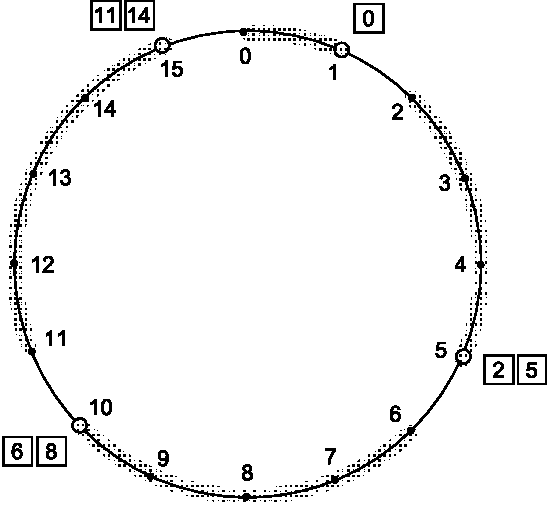
\includegraphics[width=0.4\textwidth]{pictures/pic0}\\
  \caption[Example of a $4$-bit Chord identifier circle]{Example of a $4$-bit Chord identifier circle.
  The responsibility ranges for each peer are accentuated in light gray}\label{fig:pic0}
\end{figure}
Es lassen sich auch mehrere Bilder nebeneinander platzieren wie z.B. in Abbildung
\ref{fig:multipic} zu sehen ist.
\begin{figure}[hpbt]
 \centering
  %%----start of first subfigure----
  \subfloat[FIFO size limited to 20 entries]{
   \label{fig:multipic:a} %% label for first subfigure
   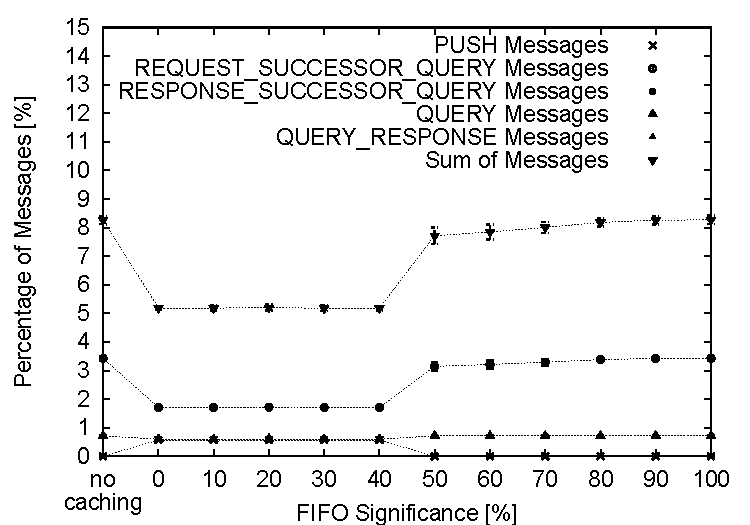
\includegraphics[width=0.48\linewidth]{pic1}}
  \hspace{0.01\textwidth}
  %%----start of second subfigure----
  \subfloat[FIFO size limited to 30 entries]{
   \label{fig:multipic:b} %% label for second subfigure
   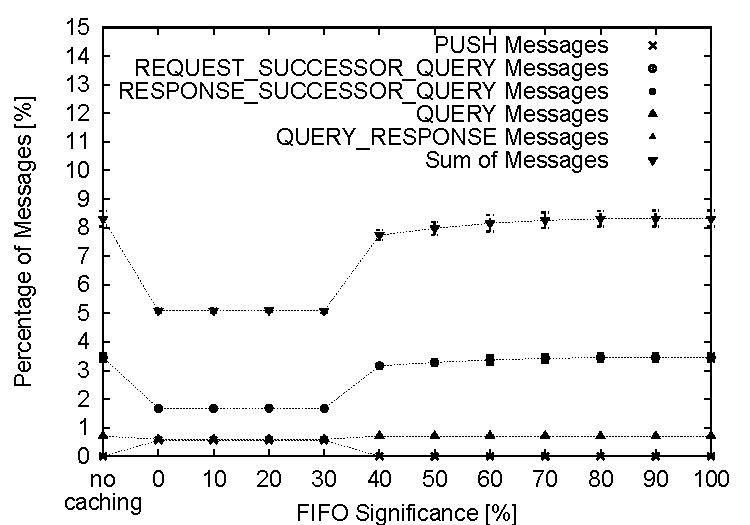
\includegraphics[width=0.48\linewidth]{pic2}}\\[0pt] % horizontal break
  %%----start of third subfigure----
  \subfloat[FIFO size limited to 40 entries]{
   \label{fig:multipic:c} %% label for third subfigure
   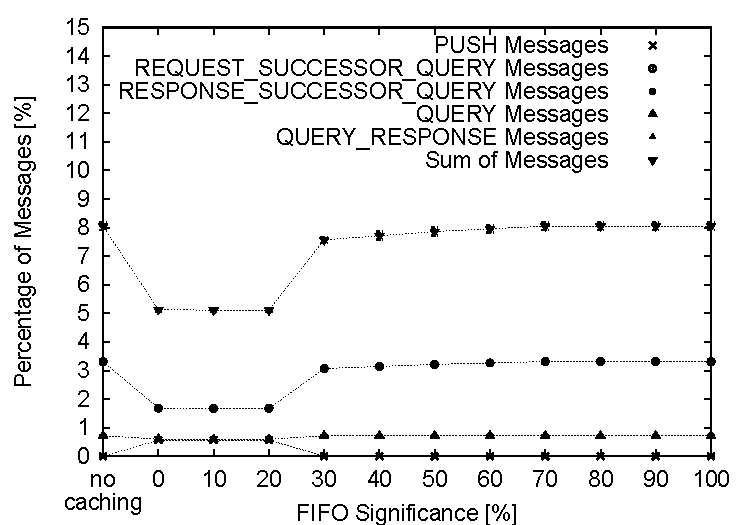
\includegraphics[width=0.48\linewidth]{pic3}}
  \hspace{0.01\textwidth}
  %%----start of fourth subfigure----
  \subfloat[FIFO size limited to 50 entries]{
   \label{fig:multipic:d} %% label for fourth subfigure
   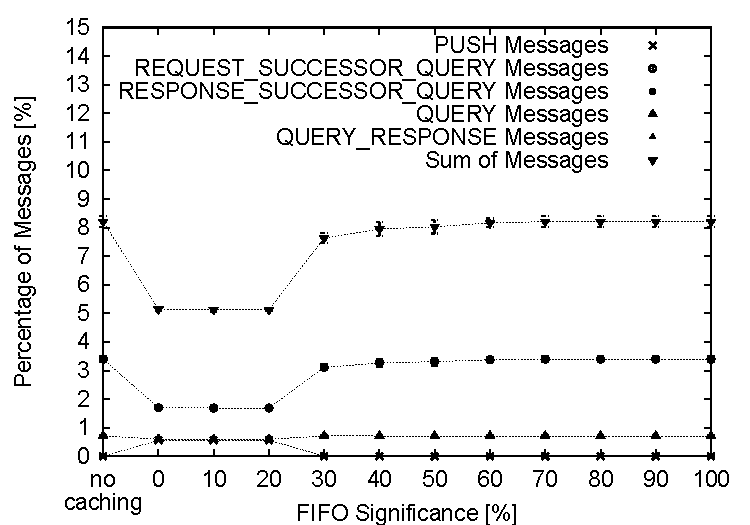
\includegraphics[width=0.48\linewidth]{pic4}}
 \caption[Observed message fractions and 95\% confidence intervals for Chord]{Observed message fractions and 95\% confidence intervals for Chord without the influence of churn. The FIFO capacity varies from 20 (\ref{fig:multipic:a}) -- 50 (\ref{fig:multipic:d}) entries (decadic steps).}
 \label{fig:multipic} %% label for entire figure
\end{figure}

\subsection{Programm Code}
Eine elegante M�glichkeit, Programmtext einzubinden, l�sst sich mit dem listings-Paket erreichen.
Das \verb|HelloWorld| Programm aus Listing \ref{lst:hw} hat in Zeile \ref{line:hw3} �brigens einen Programmierfehler.
\begin{lstlisting}[float=htp,caption=Hello World,label=lst:hw,language=Java, numbers=left, numberstyle=\tiny, stepnumber=2, numbersep=8pt, escapeinside={//@}{@//},backgroundcolor=\color{yellow},xleftmargin=3ex,xrightmargin=1ex]
public class HelloWorld {
    public static void main(String[] args) {
        Syste.out.println("Hello, World"); //@\label{line:hw3}@//
    }
}
\end{lstlisting}

\subsection{Fu�noten}
Wenn man auf Google \footnote{\url{http://www.google.com}} verweisen will, bietet sich statt einer gesonderten
Referenz auch einfach eine Fu�note an.
\subsection{Formeln}
Man kann mit \LaTeX\ sehr sch�n Formeln erzeugen:
$$L_{P}(k) = R^{orig}_{P}(k) + \sum_{i=0}^n 2*R^{i}_{P}(k)$$

% further chapters
%
% =================================================================================================
% place your appendix here
% -------------------------------------------------------------------------------------------------
%
\appendix
% -------------------------------------------------------------------------------------------------
%      MDSG Latex Framework
%      ============================================================================================
%      File:                  appendix.tex
%      Author(s):             Michael Duerr
%      Version:               1
%      Creation Date:         30. Mai 2010
%      Creation Date:         30. Mai 2010
%
%      Notes:                 - Place your appendix here
%                             - Use the same commands (`chapter', `section', ...) as in main text
% -------------------------------------------------------------------------------------------------
%
\chapter{Training Parameters}\label{ax:training_params}
\small{
    \begin{verbatim}
required arguments:
  --algo ALGO           Algorithm to use for training. Choose between 'ppo'
                        and 'dqn'.

optional arguments:
  -h, --help            show this help message and exit
  --seed SEED           Generate the same set of pseudo random constellations,
                        colors, positions, etc. every time the algorithm is
                        executed. (default: 1)
  --agents AGENTS       Amount of agents. (default: 2)
  --model MODEL         Path of the model inside the storage folder, if none
                        is given then a random name is generated. (default:
                        None)
  --capture CAPTURE     Boolean to enable capturing of the environment. The
                        outcome are in form of gifs. (default: True)
  --env ENV             Environment ID, choose between Empty-Grid-v0 for an
                        empty environment and FourRooms-Grid-v0 for an
                        environment divided into equal sized rooms. (default:
                        Empty-Grid-v0)
  --agent-view-size AGENT_VIEW_SIZE
                        Grid size the agent can see. Agent Observation is
                        based on that field of view. For example, 7x7 grid
                        size means agent can see three tiles in each
                        direction. (default: 7)
  --grid-size GRID_SIZE
                        Size of the environment grid. (default: 5)
  --max-steps MAX_STEPS
                        Maximum amount of steps an agent has to reach a goal.
                        If none is given then this max count is set to: grid
                        size * grid size. (default: None)
  --setting SETTING     Setting can be either: '' for cooperation, 'mixed-
                        motive' for a mixed motive environment, 'mixed-motive-
                        competitive' for a competitive composition or
                        'difference-reward' for a setting that calculates
                        difference rewards. Cooperation means all agents get
                        the same reward. If set to mixed-motive or mixed-
                        motive-competitve the reward is not shared and each
                        agent is responsible for its own success. In
                        competitive mode, agents can take over opponent
                        coloration without resetting the cells, otherwise
                        cells are always reset when colored and walked over.
                        The last option 'difference-reward' is a cooperation
                        setting but calculates the reward for each agent by
                        subtracting a new reward from the total reward. The
                        new reward just excludes the action of this one agent.
                        A high difference reward means, that the action of
                        that agent was good. (default: '' for cooperation)
  --market MARKET       There are three options: 'sm', 'am' and '' for none.
                        SM = Shareholder Market where agents can sell or buy
                        shares on the market. AM = Action Market where agents
                        can buy specific actions from others. (default = '')
  --trading-fee TRADING_FEE
                        If a market transaction is executed, this value
                        determines the price, i.e. in an action market this
                        defines the price the buyer pays. In a shareholder
                        market this value defines the share value. (default:
                        0.1)
  --frames FRAMES       Number of frames of training. (default: 80.000)
  --frames-per-proc FRAMES_PER_PROC
                        Number of frames per process. In case of PPO this is
                        the number of steps, before the model is optimized.
                        (default: 128)
  --procs PROCS         Number of processes/environments running parallel.
                        (default: 16)
  --recurrence RECURRENCE
                        Number of time-steps the gradient is back propagated.
                        If it is greater than one, a LSTM is added to the
                        model to have memory. (default: 1)
  --batch-size BATCH_SIZE
                        Batch size that is used for sampling. (default: 64)
  --gamma GAMMA         Discount factor with 0 <= gamma < 1, specify how
                        important future estimated rewards are. High value
                        means high importance. (default: 0.99)
  --log-interval LOG_INTERVAL
                        Number of frames between two logs. (default: 1)
  --save-interval SAVE_INTERVAL
                        Number of times the --frames-per-proc amount of frames
                        needs to be reached, to log the current training
                        values, i.e. rewards, into a csv file. (default: 10, 0
                        means no saving)
  --capture-interval CAPTURE_INTERVAL
                        Number of times --frames-per-proc amount of frames
                        needs to be reached, to capture the last --capture-
                        frames amount of steps into a gif. Warning: --capture
                        needs to be set to True as well. (default: 10, 0 means
                        no capturing)
  --capture-frames CAPTURE_FRAMES
                        Number of frames that are captured. (default: 50, 0
                        means no capturing)
  --lr LR               Learning rate. (default: 0.001)
  --optim-eps OPTIM_EPS
                        Epsilon value for the Adam optimizer. (default: 1e-8)
  --epochs EPOCHS       [PPO] Number of epochs for PPO optimization. (default:
                        4)
  --gae-lambda GAE_LAMBDA
                        [PPO] Lambda coefficient in GAE formula, used for
                        calculation of the advantage values. (default: 0.95, 1
                        means no gae)
  --entropy-coef ENTROPY_COEF
                        [PPO] Entropy term coefficient. (default: 0.01)
  --value-loss-coef VALUE_LOSS_COEF
                        [PPO] Value loss term coefficient. (default: 0.5)
  --max-grad-norm MAX_GRAD_NORM
                        [PPO] Maximum norm of gradient. (default: 0.5)
  --clip-eps CLIP_EPS   [PPO] Clipping epsilon for PPO. (default: 0.2)
  --epsilon-start EPSILON_START
                        [DQN] Starting value of epsilon, used for action
                        selection. (default: 1.0 -> high exploration)
  --epsilon-end EPSILON_END
                        [DQN] Ending value of epsilon, used for action
                        selection. (default: 0.01 -> high exploitation)
  --epsilon-decay EPSILON_DECAY
                        [DQN] Controls the rate of the epsilon decay in order
                        to shift from exploration to exploitation. The higher
                        the value the slower epsilon decays. (default: 5.000)
  --replay-size REPLAY_SIZE
                        [DQN] Size of the replay memory. (default: 40.000)
  --initial-target-update INITIAL_TARGET_UPDATE
                        [DQN] Frames until the target network is updated,
                        Needs to be smaller than --target-update! (default:
                        1.000)
  --target-update TARGET_UPDATE
                        [DQN] Frames between updating the target network,
                        Needs to be smaller or equal to --frames-per-proc and
                        bigger than --initial-target-update! (default: 15.000)
    \end{verbatim}
}


\chapter{Detailed Results}\label{ax:plots}

\subsection{Easy Environment}
The following plots show all details of the best training results in a small 5x5 grid. The default parameters of Appendix \ref{ax:training_params} are used for all executions. Only the agent amount, setting and market value change. In the first Figure \ref{fig:ax-easy-1}, one agent is acting in the environment, all other trainings are executed with two agents. For details see Chapter \ref{sec:Results}. An example to run a training process is shown below.

\begin{lstlisting}[float=htp,language=bash, escapeinside={//@}{@//},xleftmargin=3ex,xrightmargin=1ex]
$ python -m scripts.train
    --algo ppo
    --model ppo-easy
    --agents 2
\end{lstlisting}

\newpage
\vfill
% [!hpbt]
\begin{figure}
    \centering
    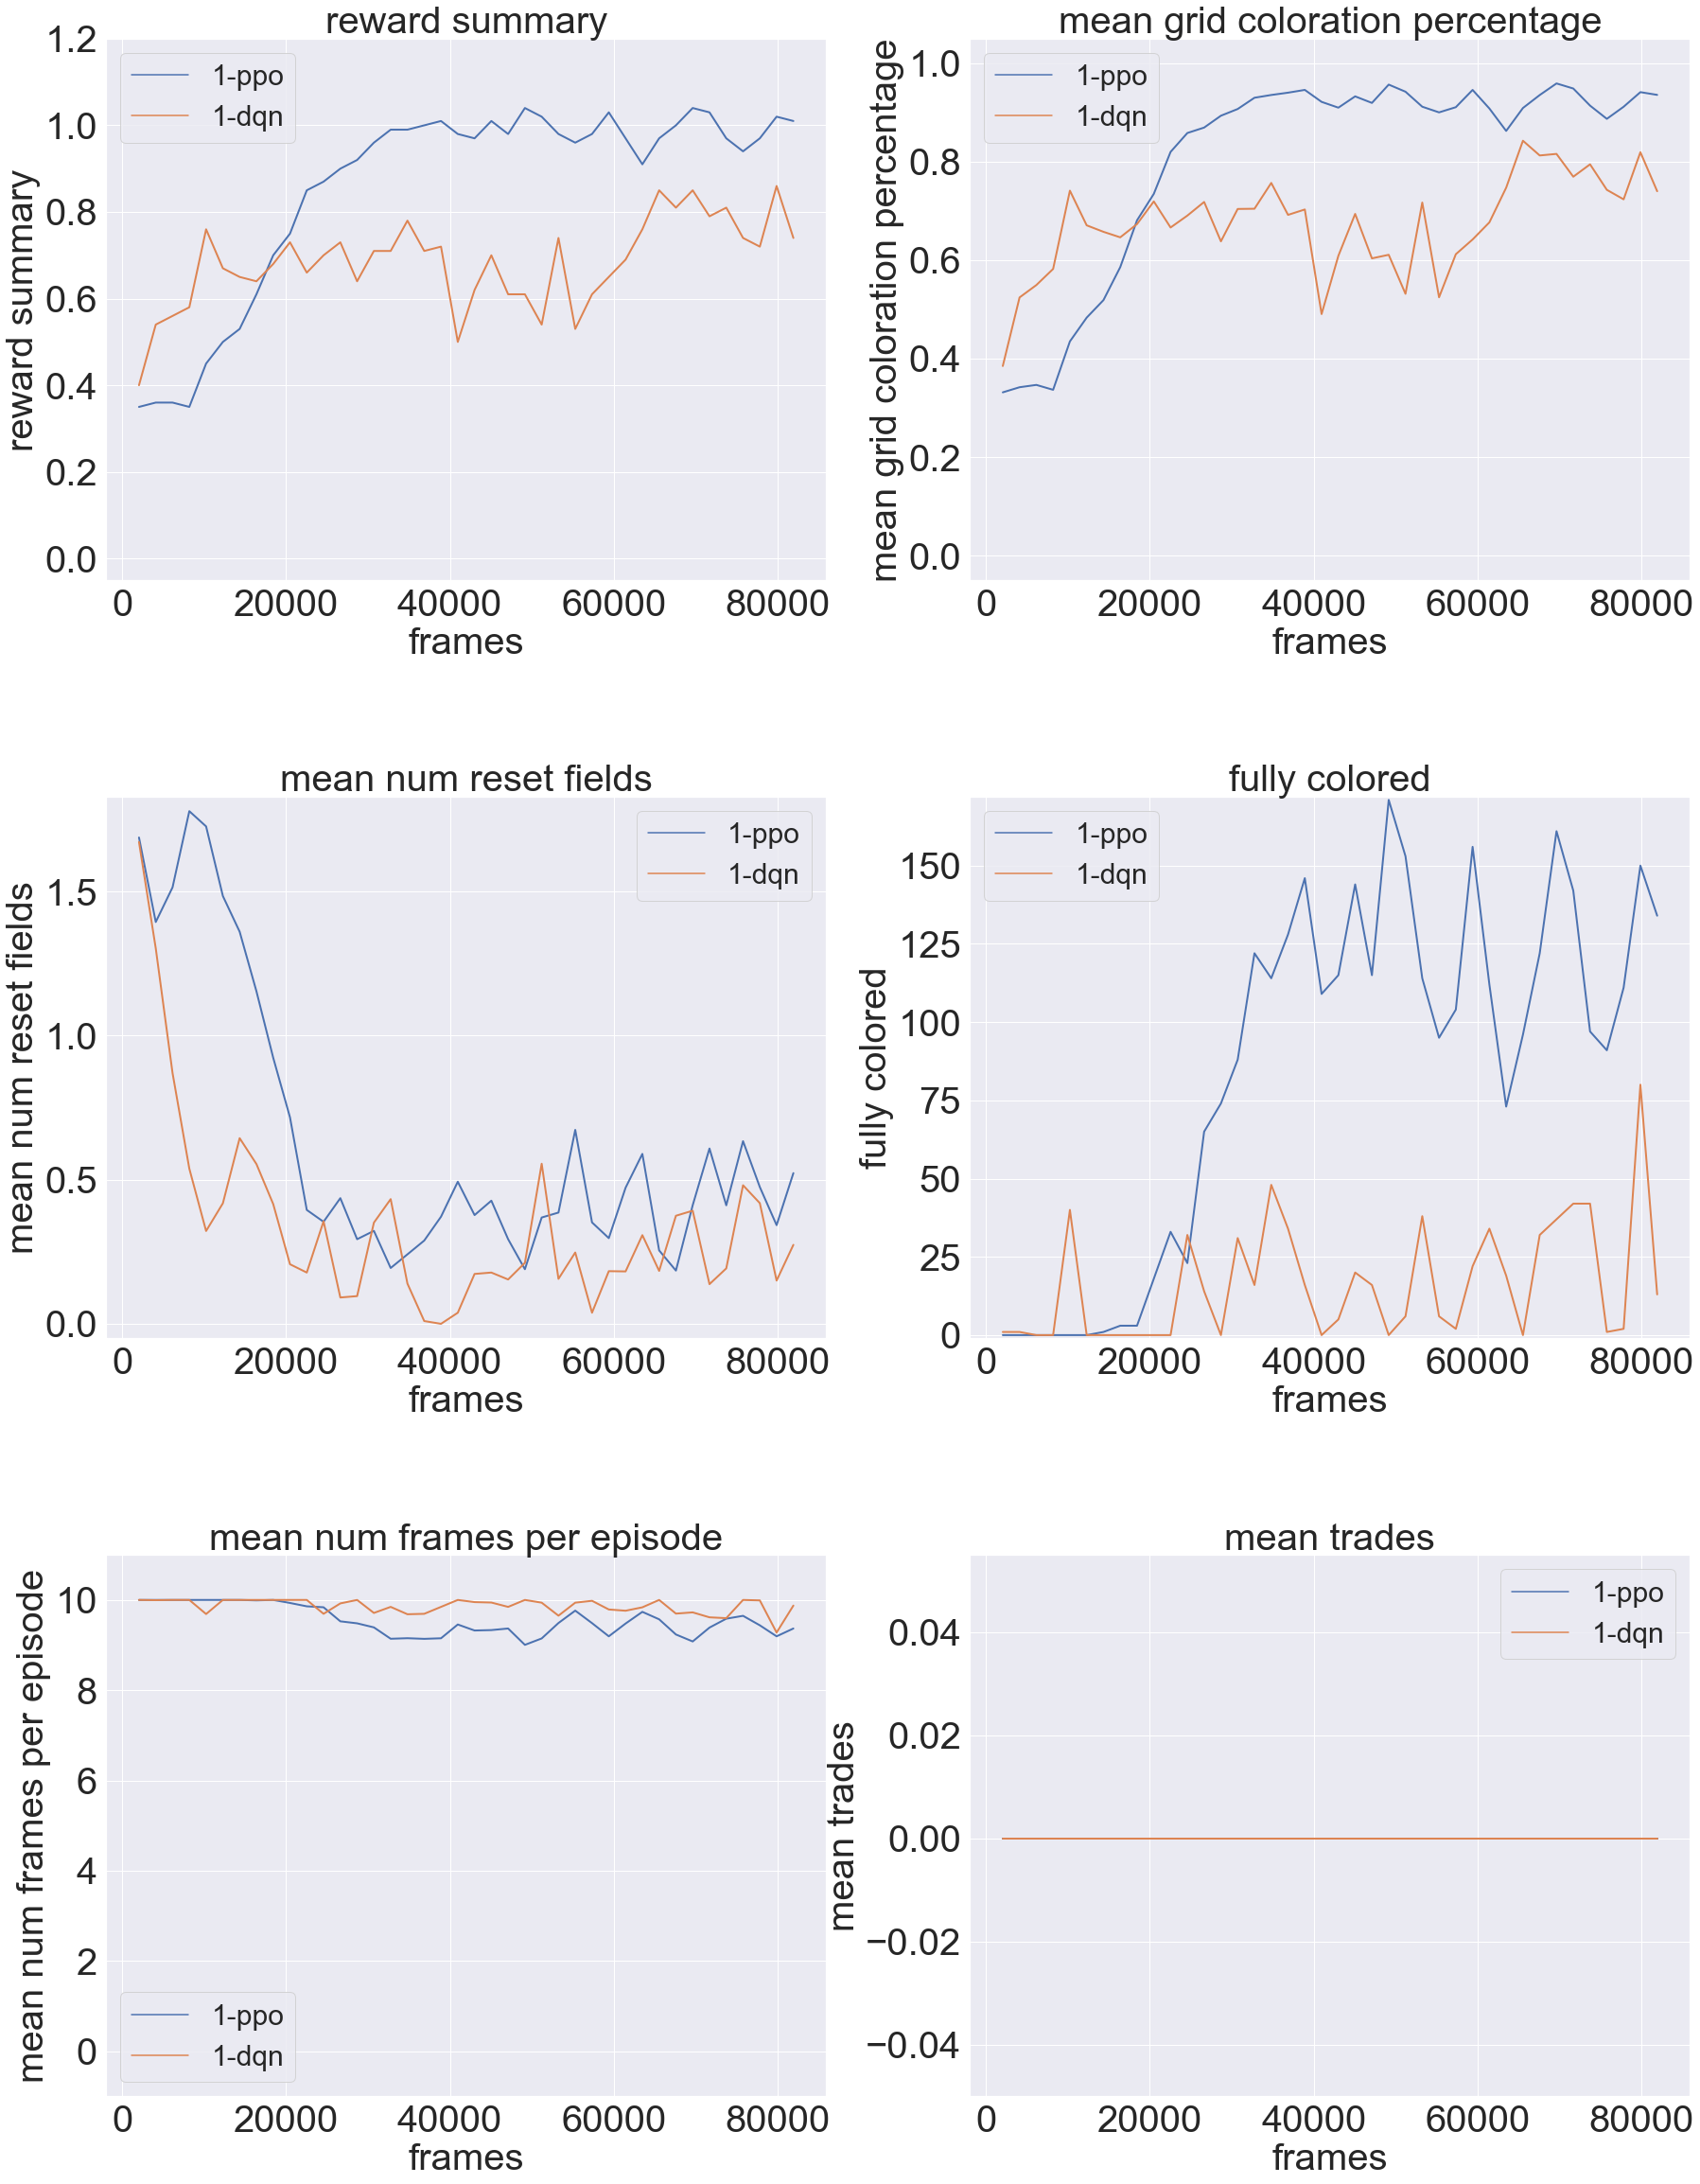
\includegraphics[width=1\textwidth]{AX-easy-1.png}\\
    \caption[PPO and DQN Training Details with One Agent]{Details of the training with one agent using PPO and DQN}\label{fig:ax-easy-1}
\end{figure}
\vfill
\clearpage


\newpage
\vfill
\begin{figure}
    \centering
    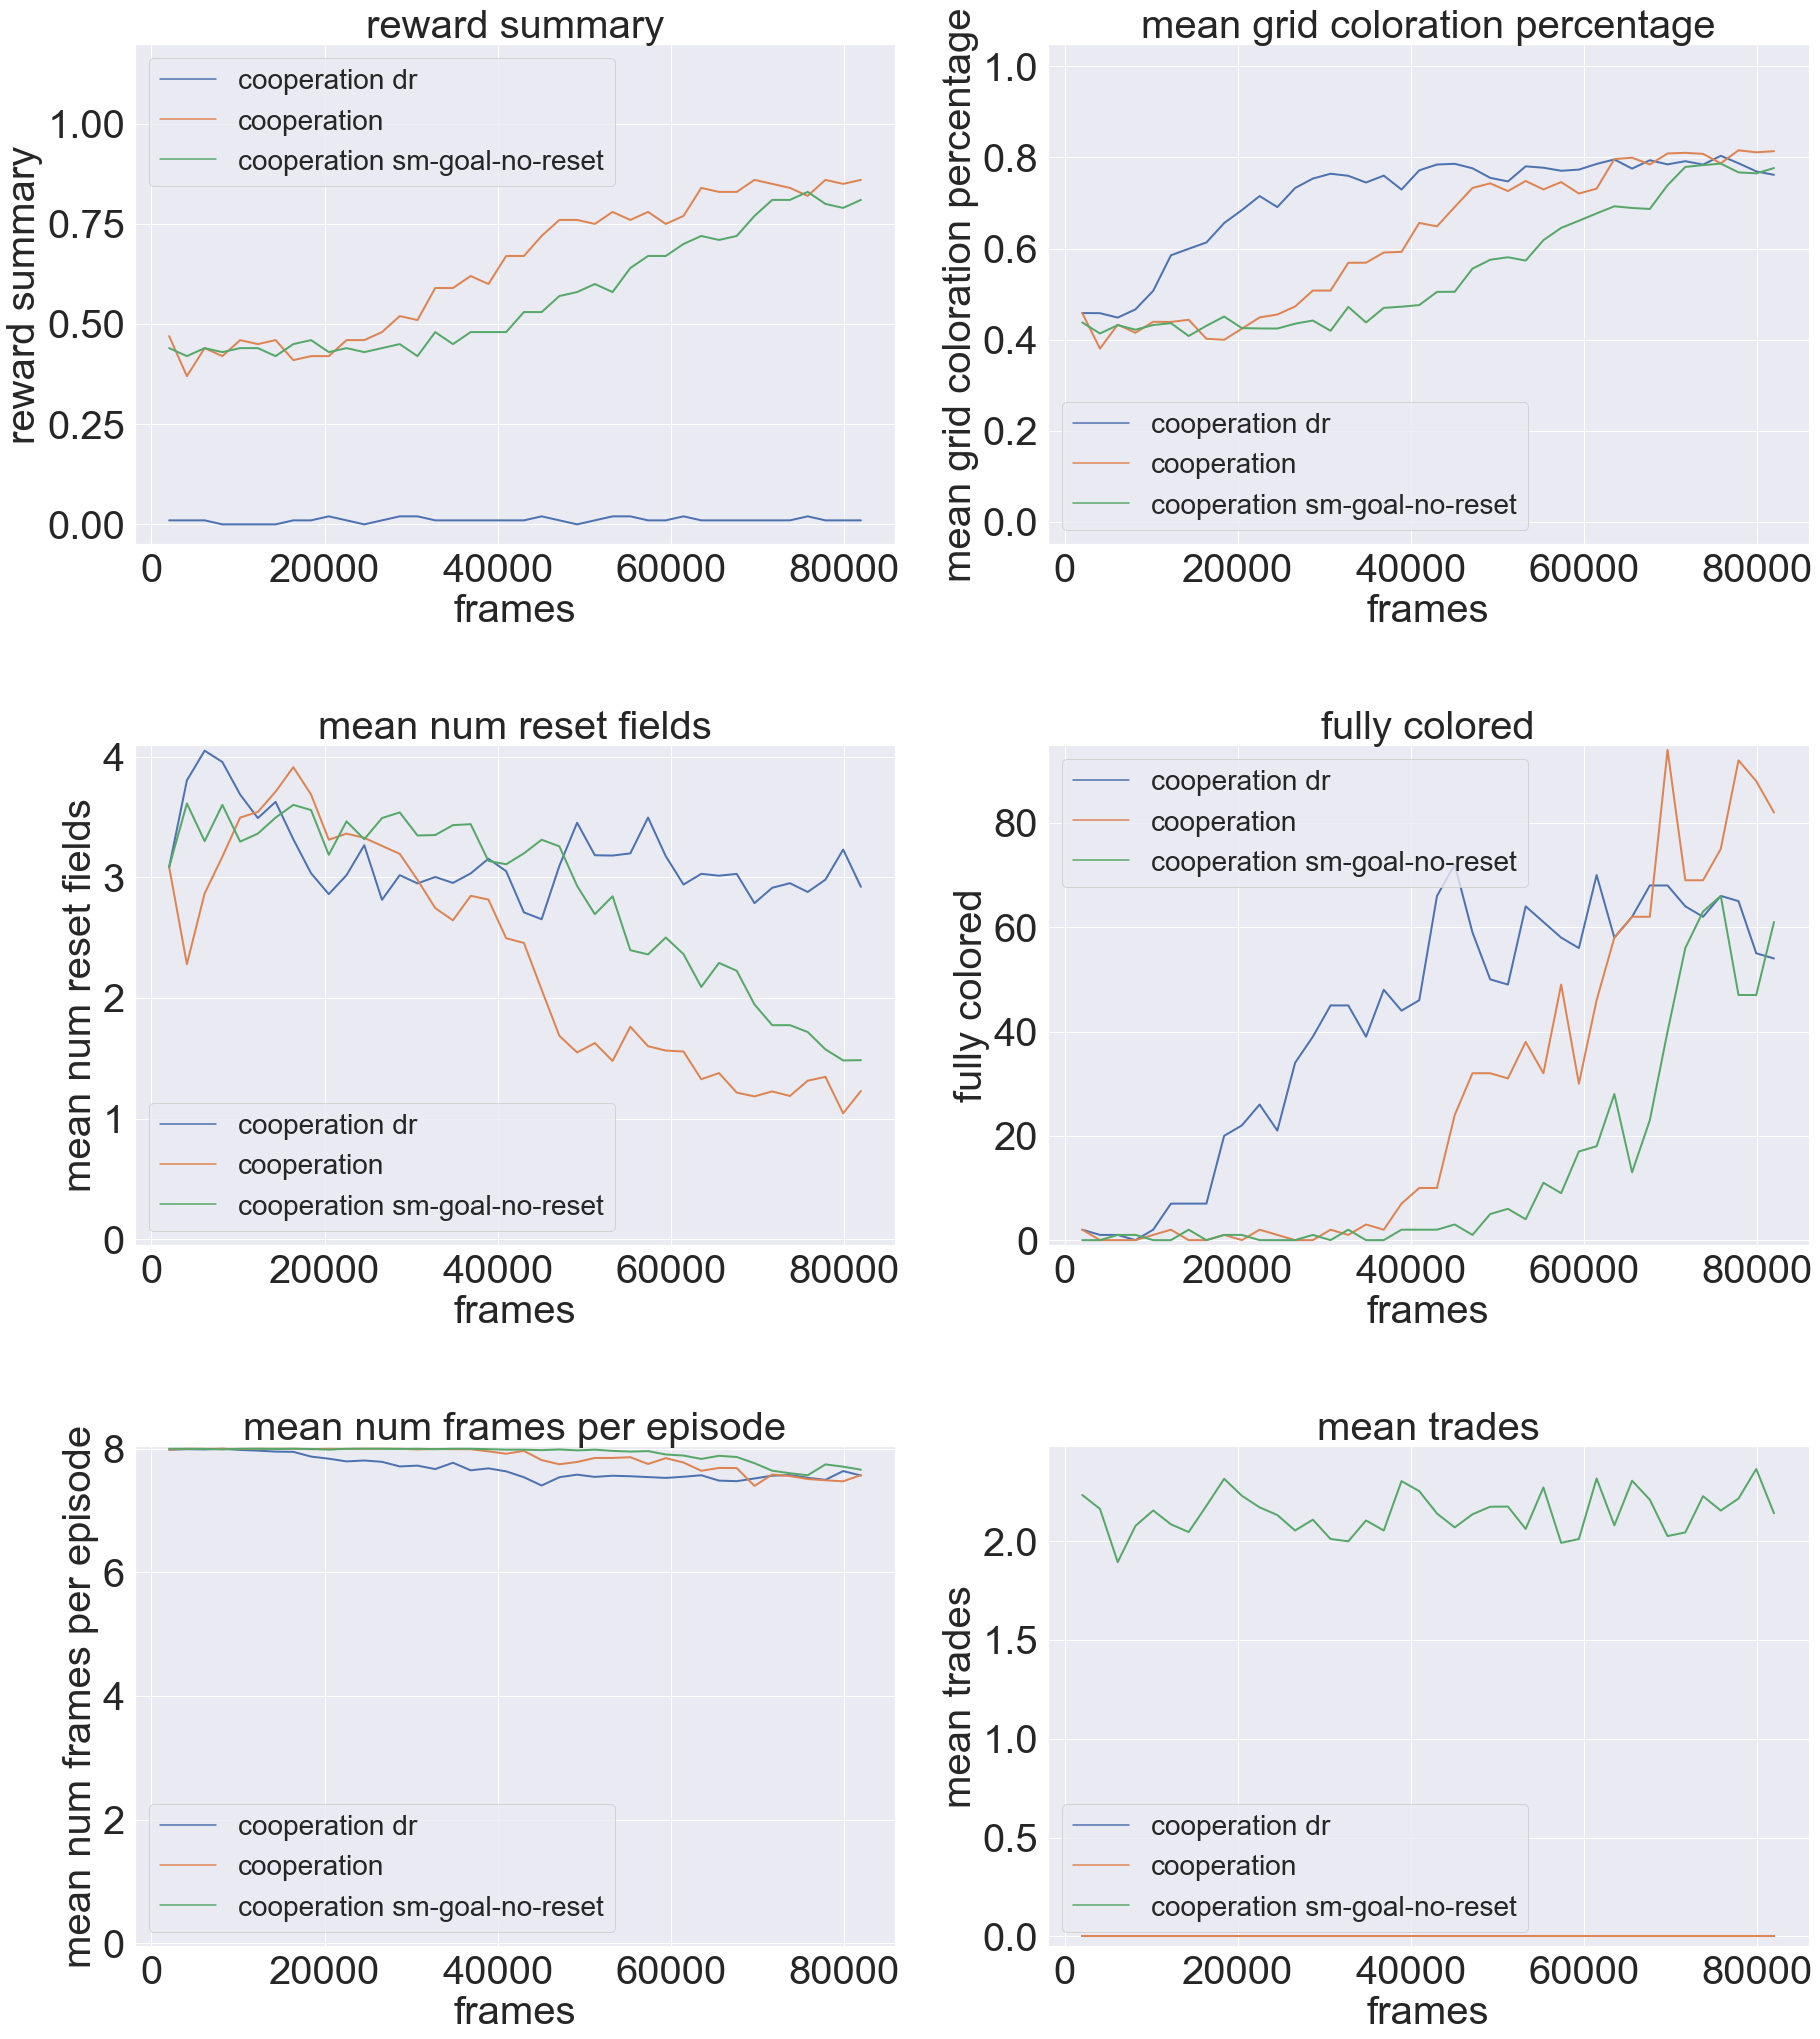
\includegraphics[width=1\textwidth]{AX-easy-2-ppo-coop.png}\\
    \caption[Training Details of Top PPO Cooperation Executions]{Top cooperation score details of two PPO agents}\label{fig:ax-easy-2-ppo-coop}
\end{figure}
\vfill
\clearpage


\newpage
\vfill
\begin{figure}
    \centering
    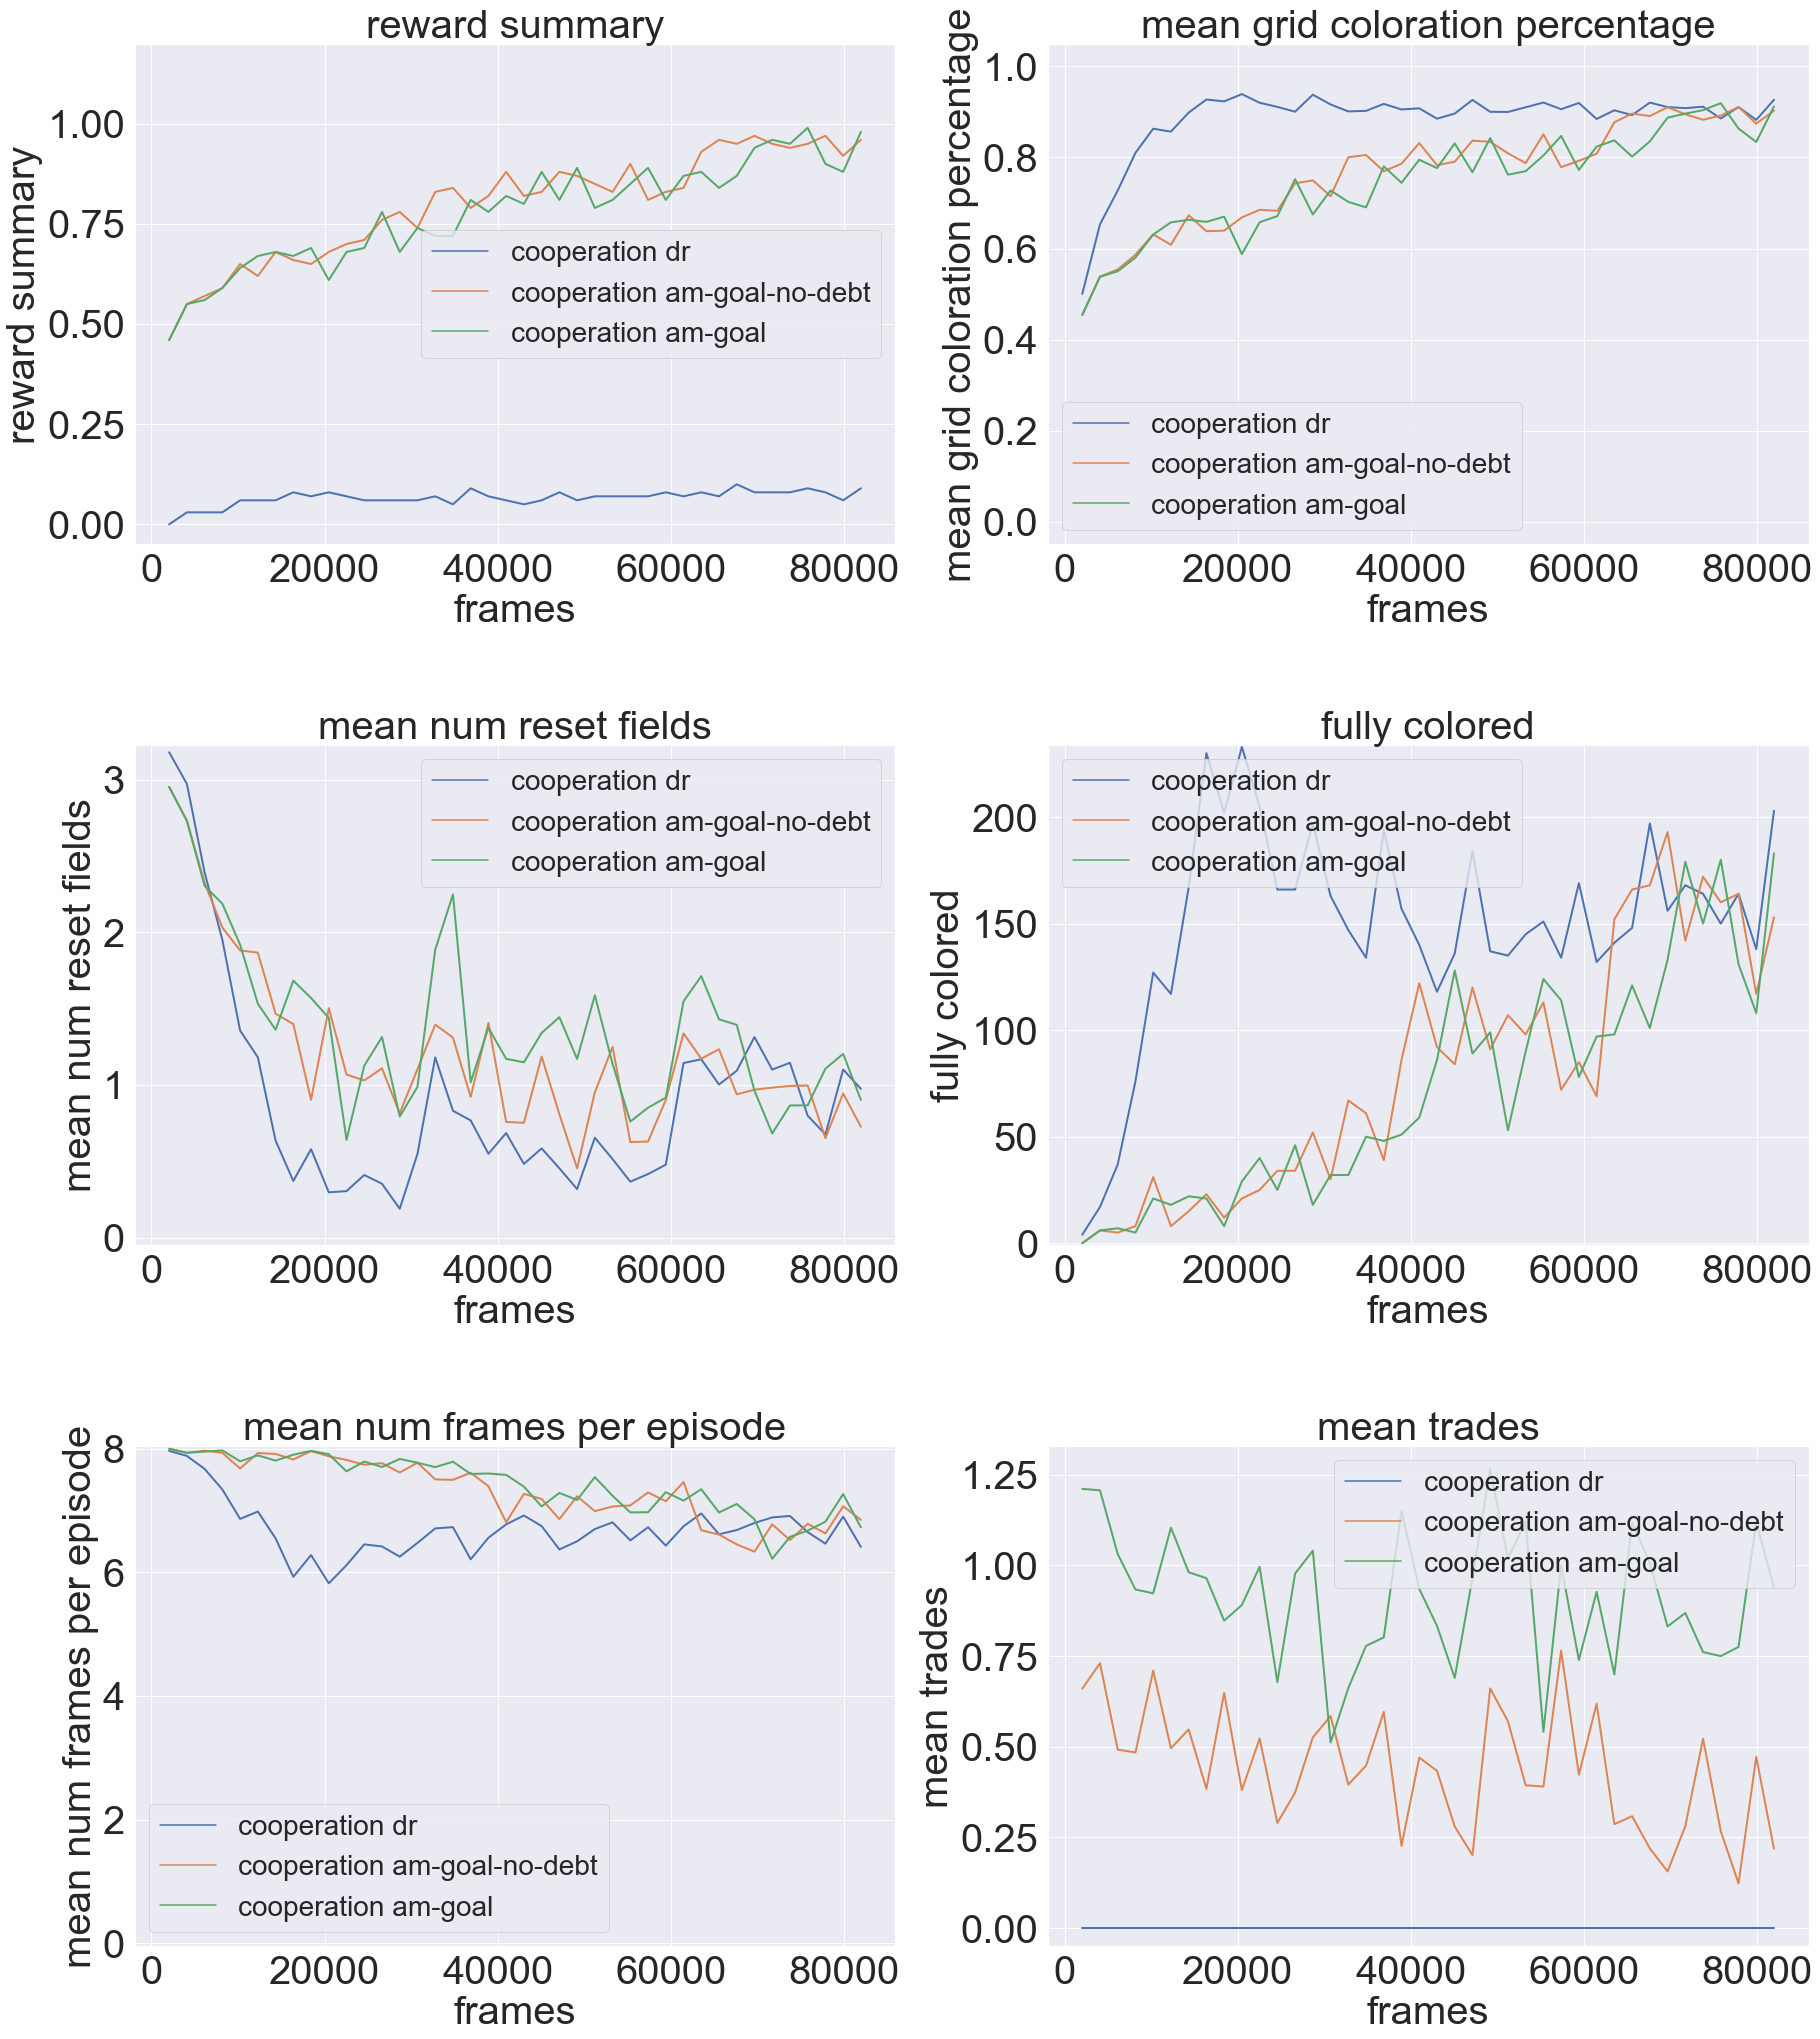
\includegraphics[width=1\textwidth]{AX-easy-2-dqn-coop.png}\\
    \caption[Training Details of Top DQN Cooperation Executions]{Top cooperation score details of two DQN agents}\label{fig:ax-easy-2-dqn-coop}
\end{figure}
\vfill
\clearpage


\newpage
\vfill
\begin{figure}
    \centering
    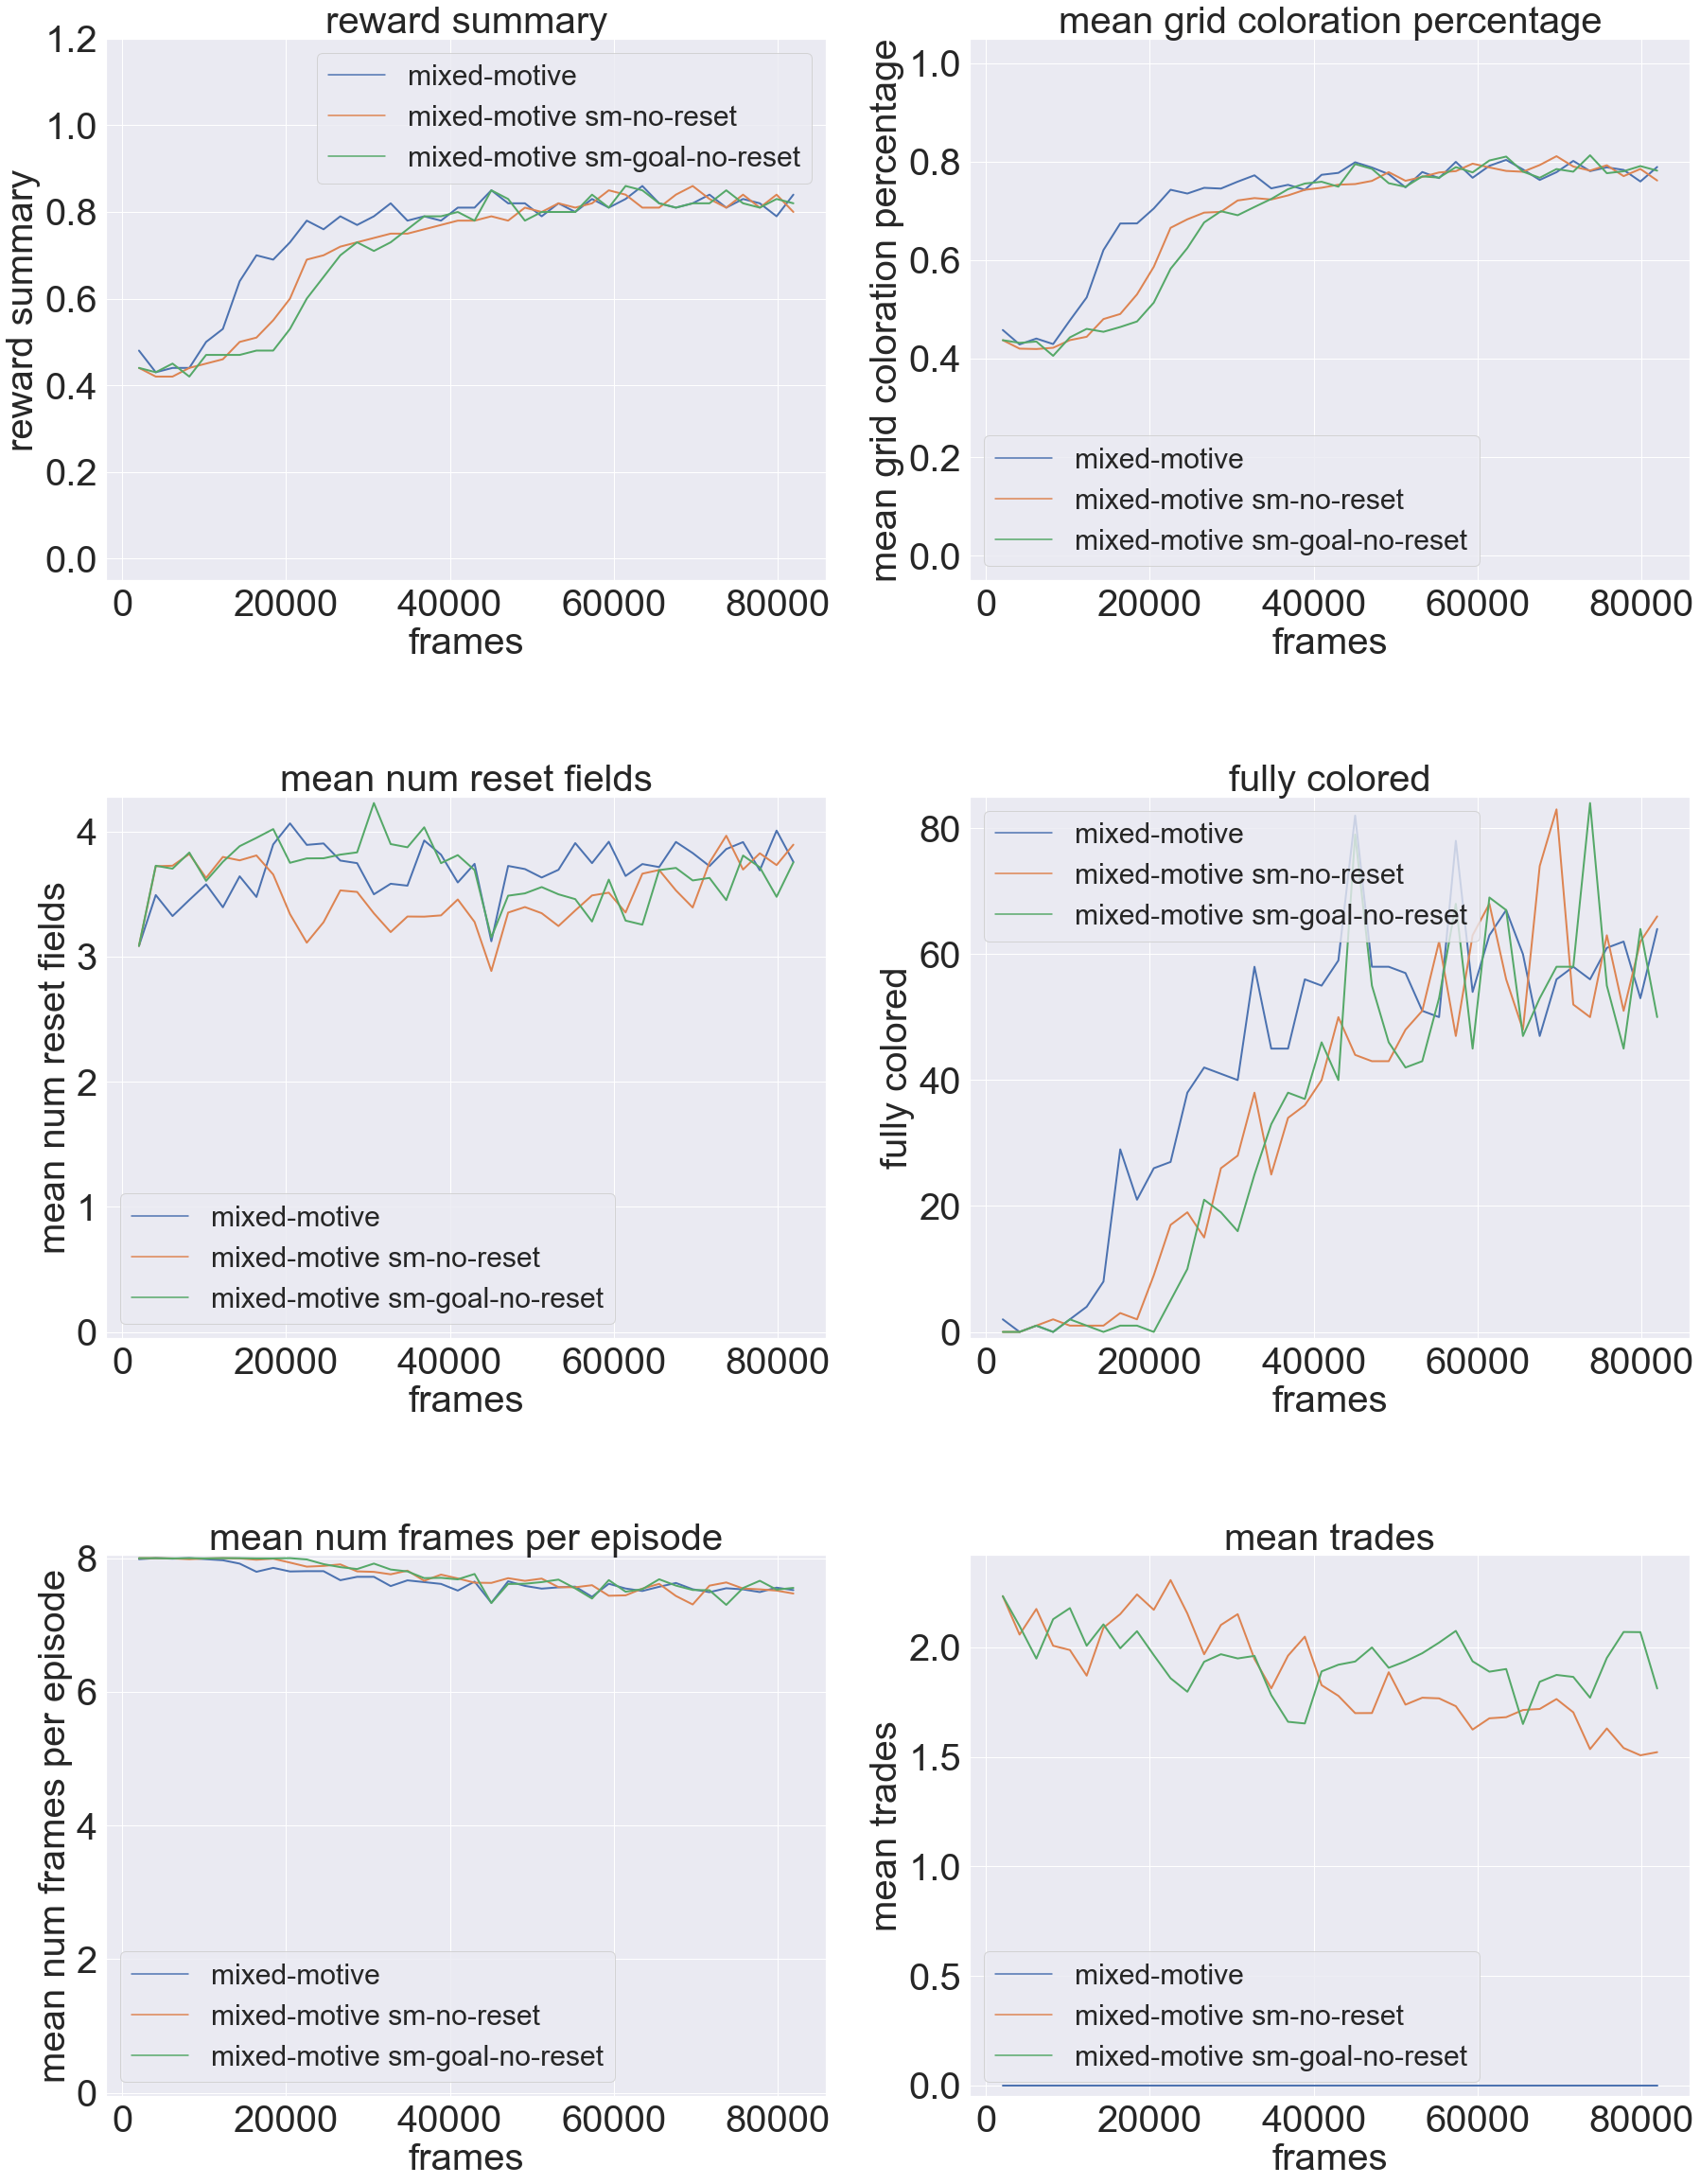
\includegraphics[width=1\textwidth]{AX-easy-2-ppo-mixed.png}\\
    \caption[Training Details of Top PPO Mixed-Motive Executions]{Top mixed-motive score details of two PPO agents}\label{fig:ax-easy-2-ppo-mixed}
\end{figure}
\vfill
\clearpage


\newpage
\vfill
\begin{figure}
    \centering
    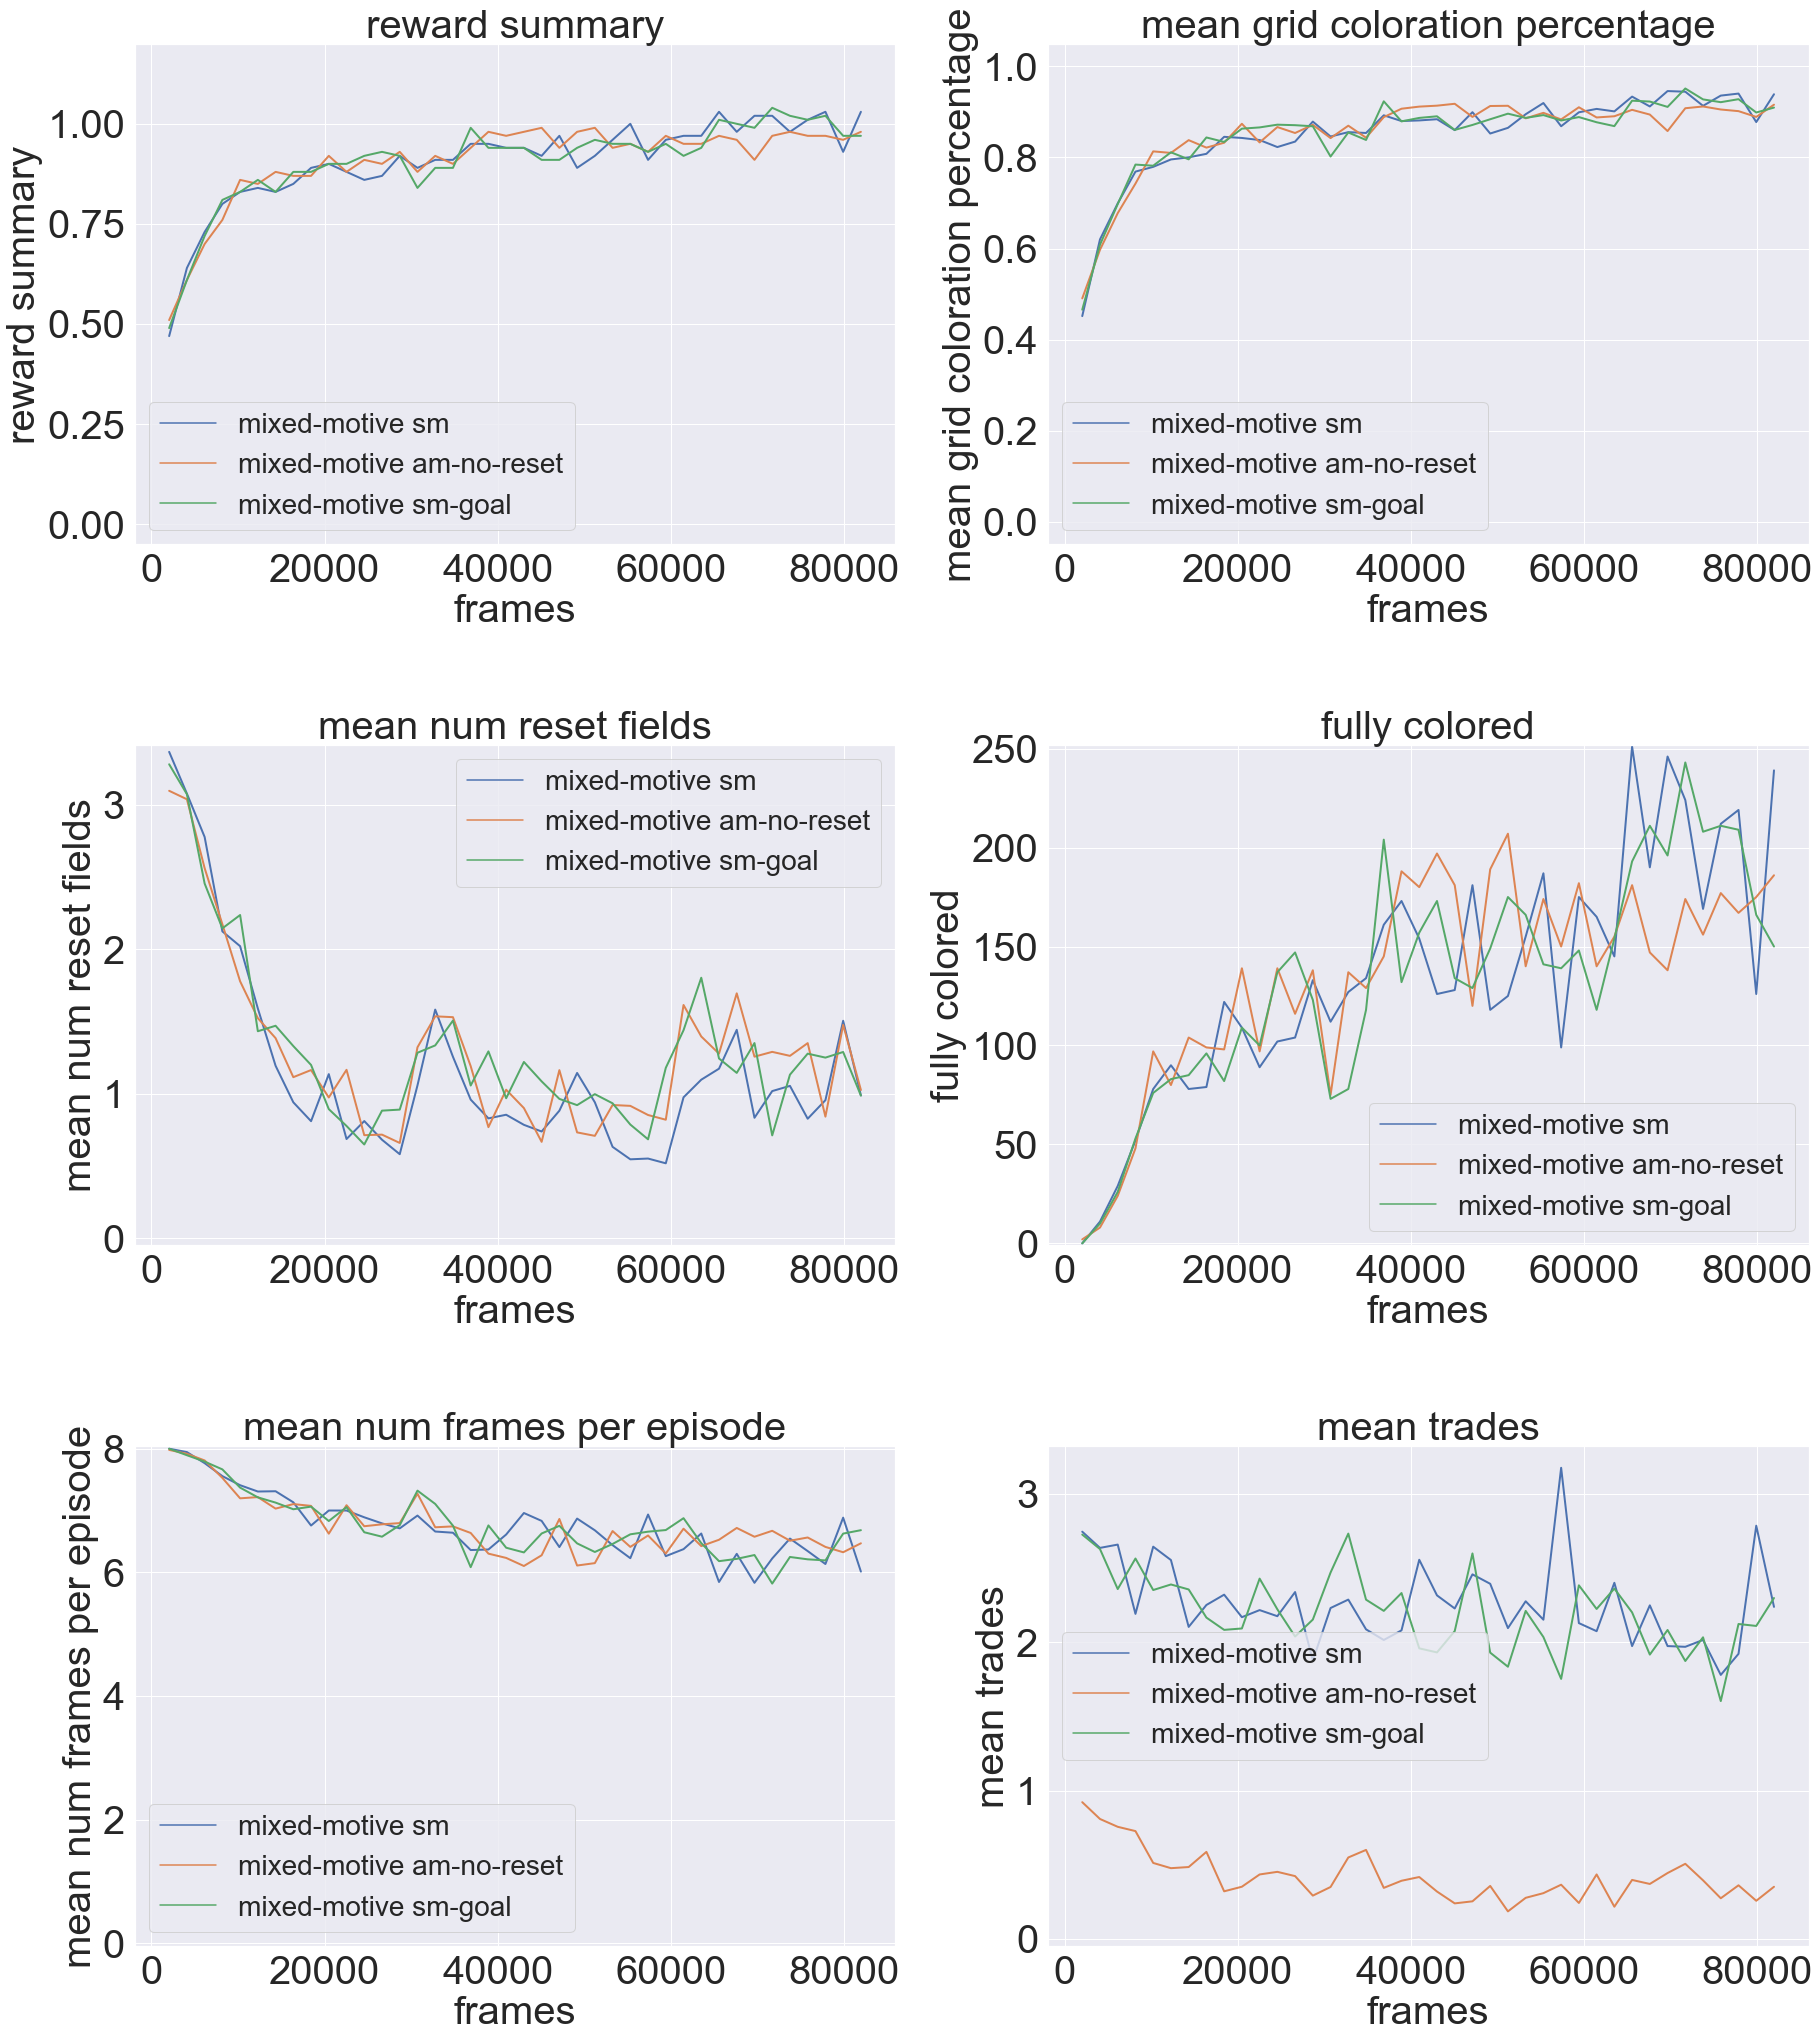
\includegraphics[width=1\textwidth]{AX-easy-2-dqn-mixed.png}\\
    \caption[Training Details of Top DQN Mixed-Motive Executions]{Top mixed-motive score details of two DQN agents}\label{fig:ax-easy-2-dqn-mixed}
\end{figure}
\vfill
\clearpage


\newpage
\vfill
\begin{figure}
    \centering
    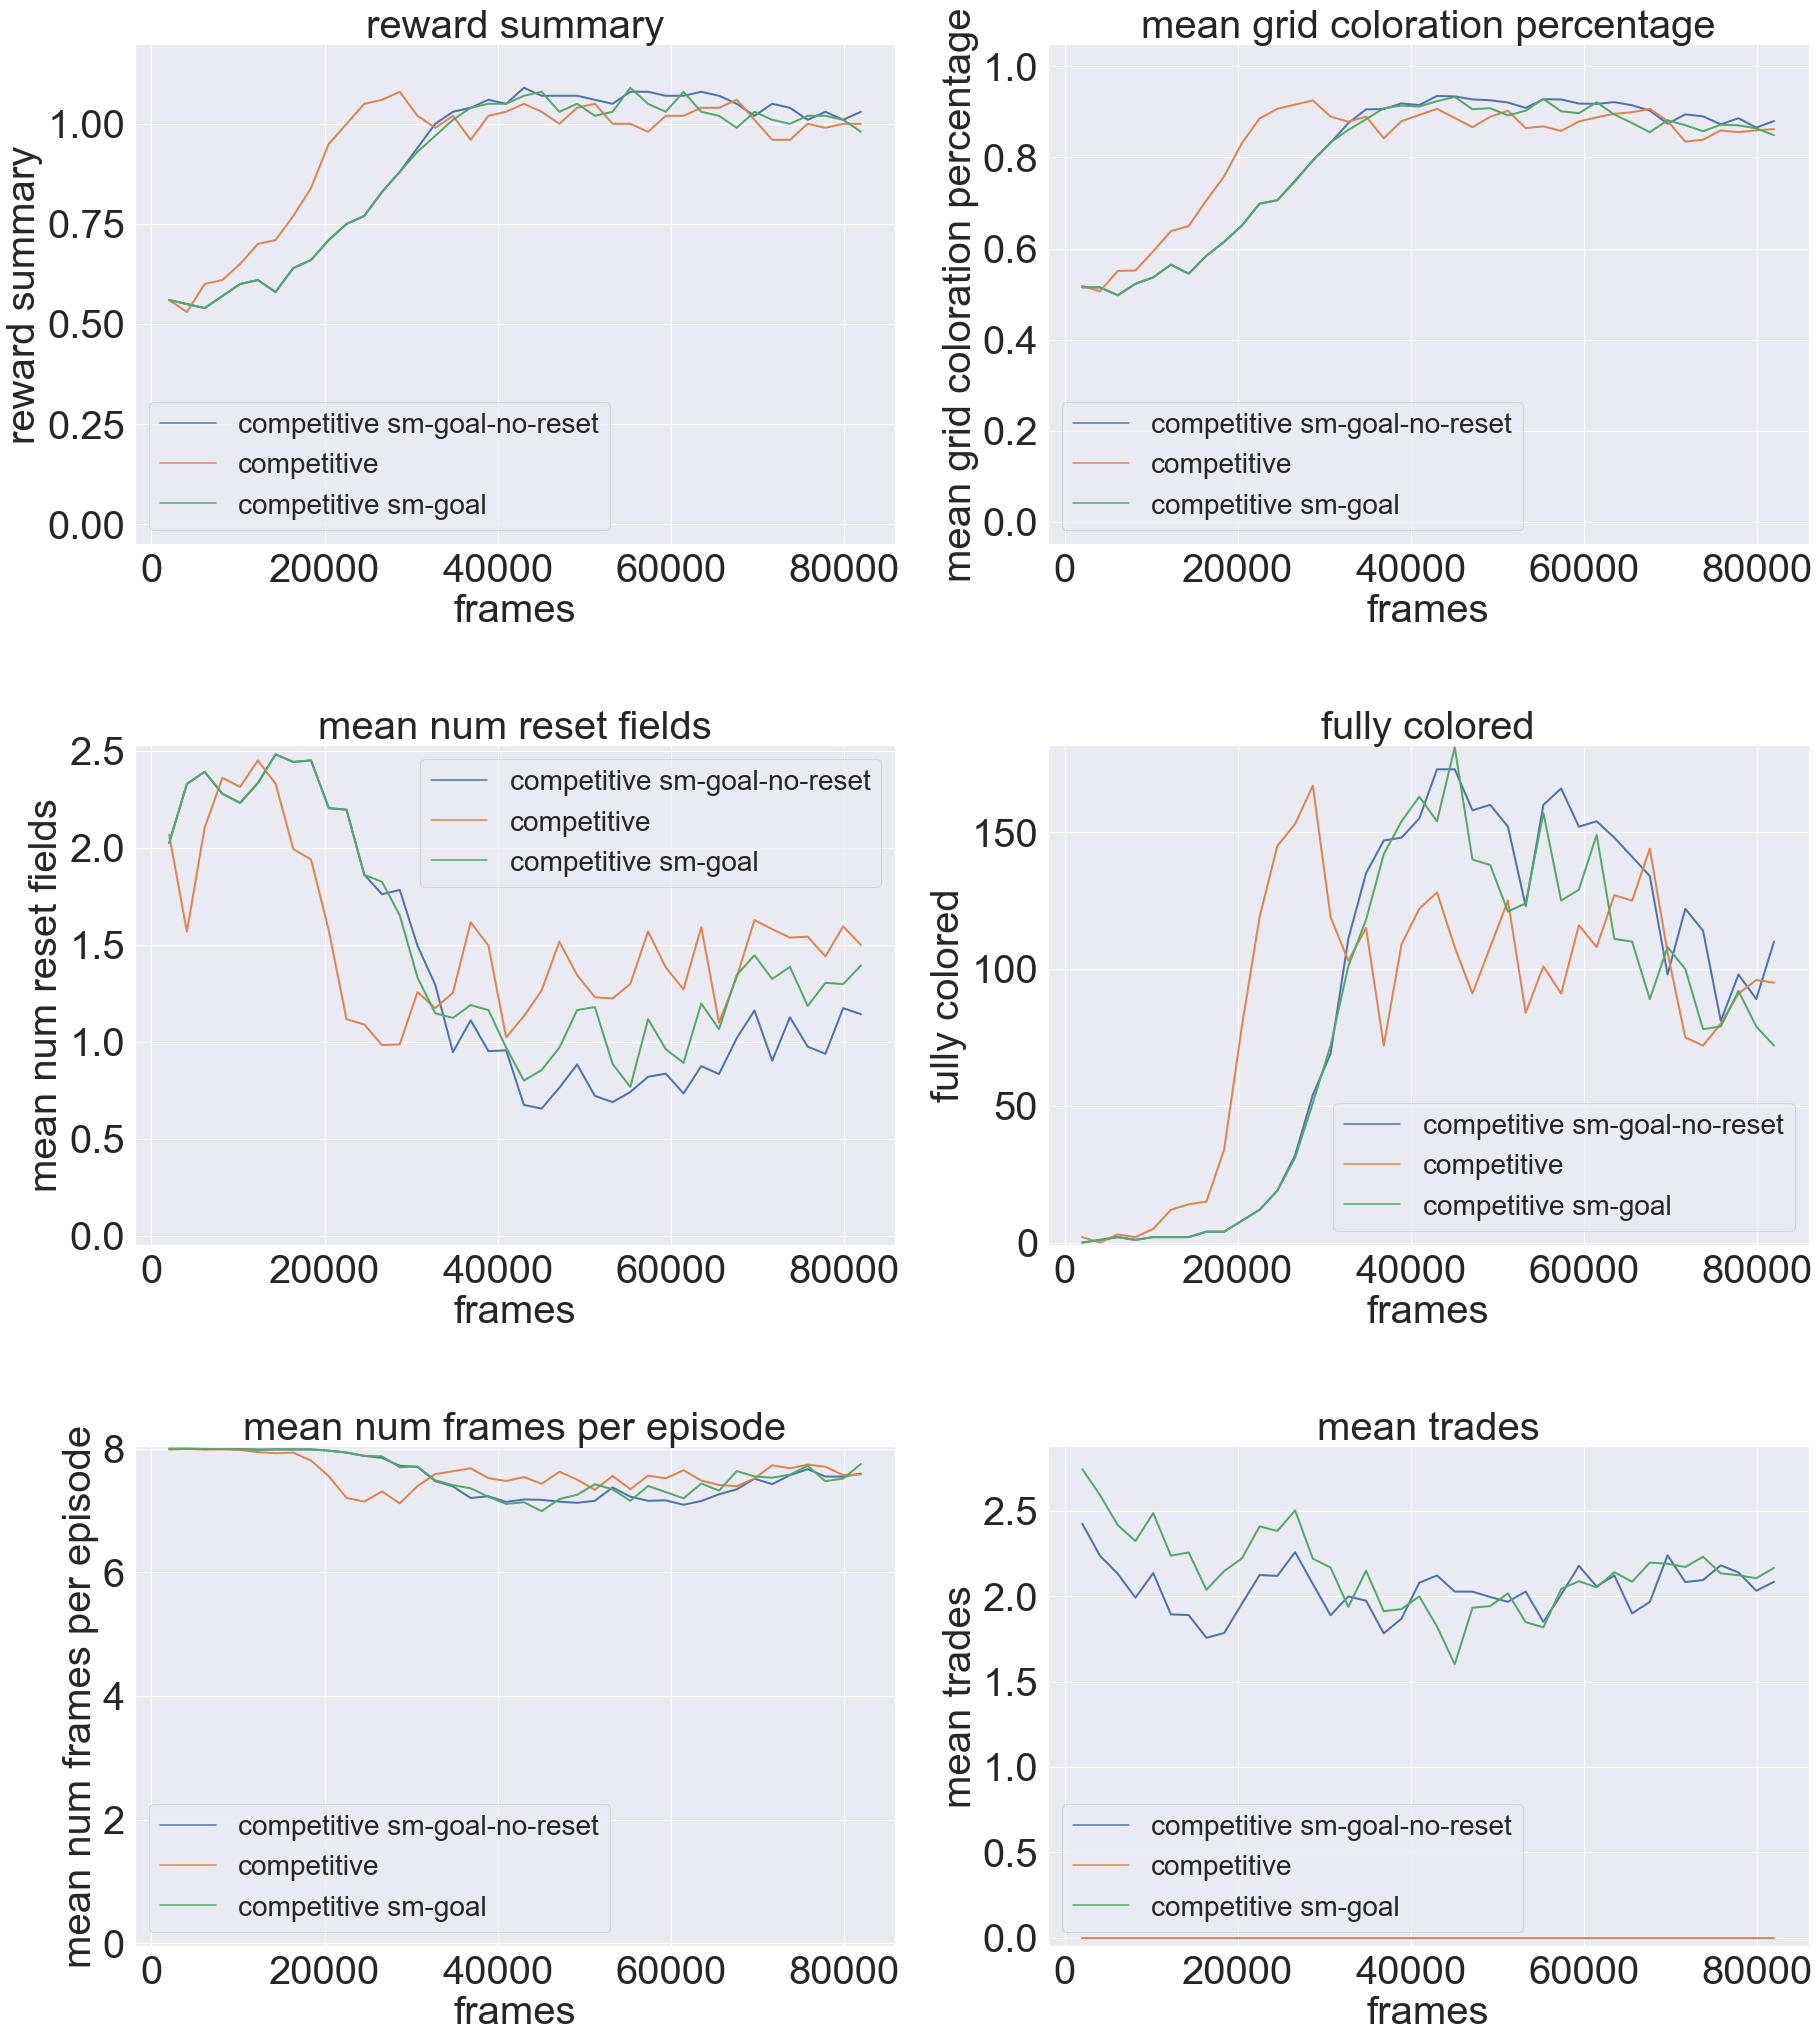
\includegraphics[width=1\textwidth]{AX-easy-2-ppo-comp.png}\\
    \caption[Training Details of Top PPO Competitive Executions]{Top competitive score details of two PPO agents}\label{fig:ax-easy-2-ppo-comp}
\end{figure}
\vfill
\clearpage


\newpage
\vfill
\begin{figure}
    \centering
    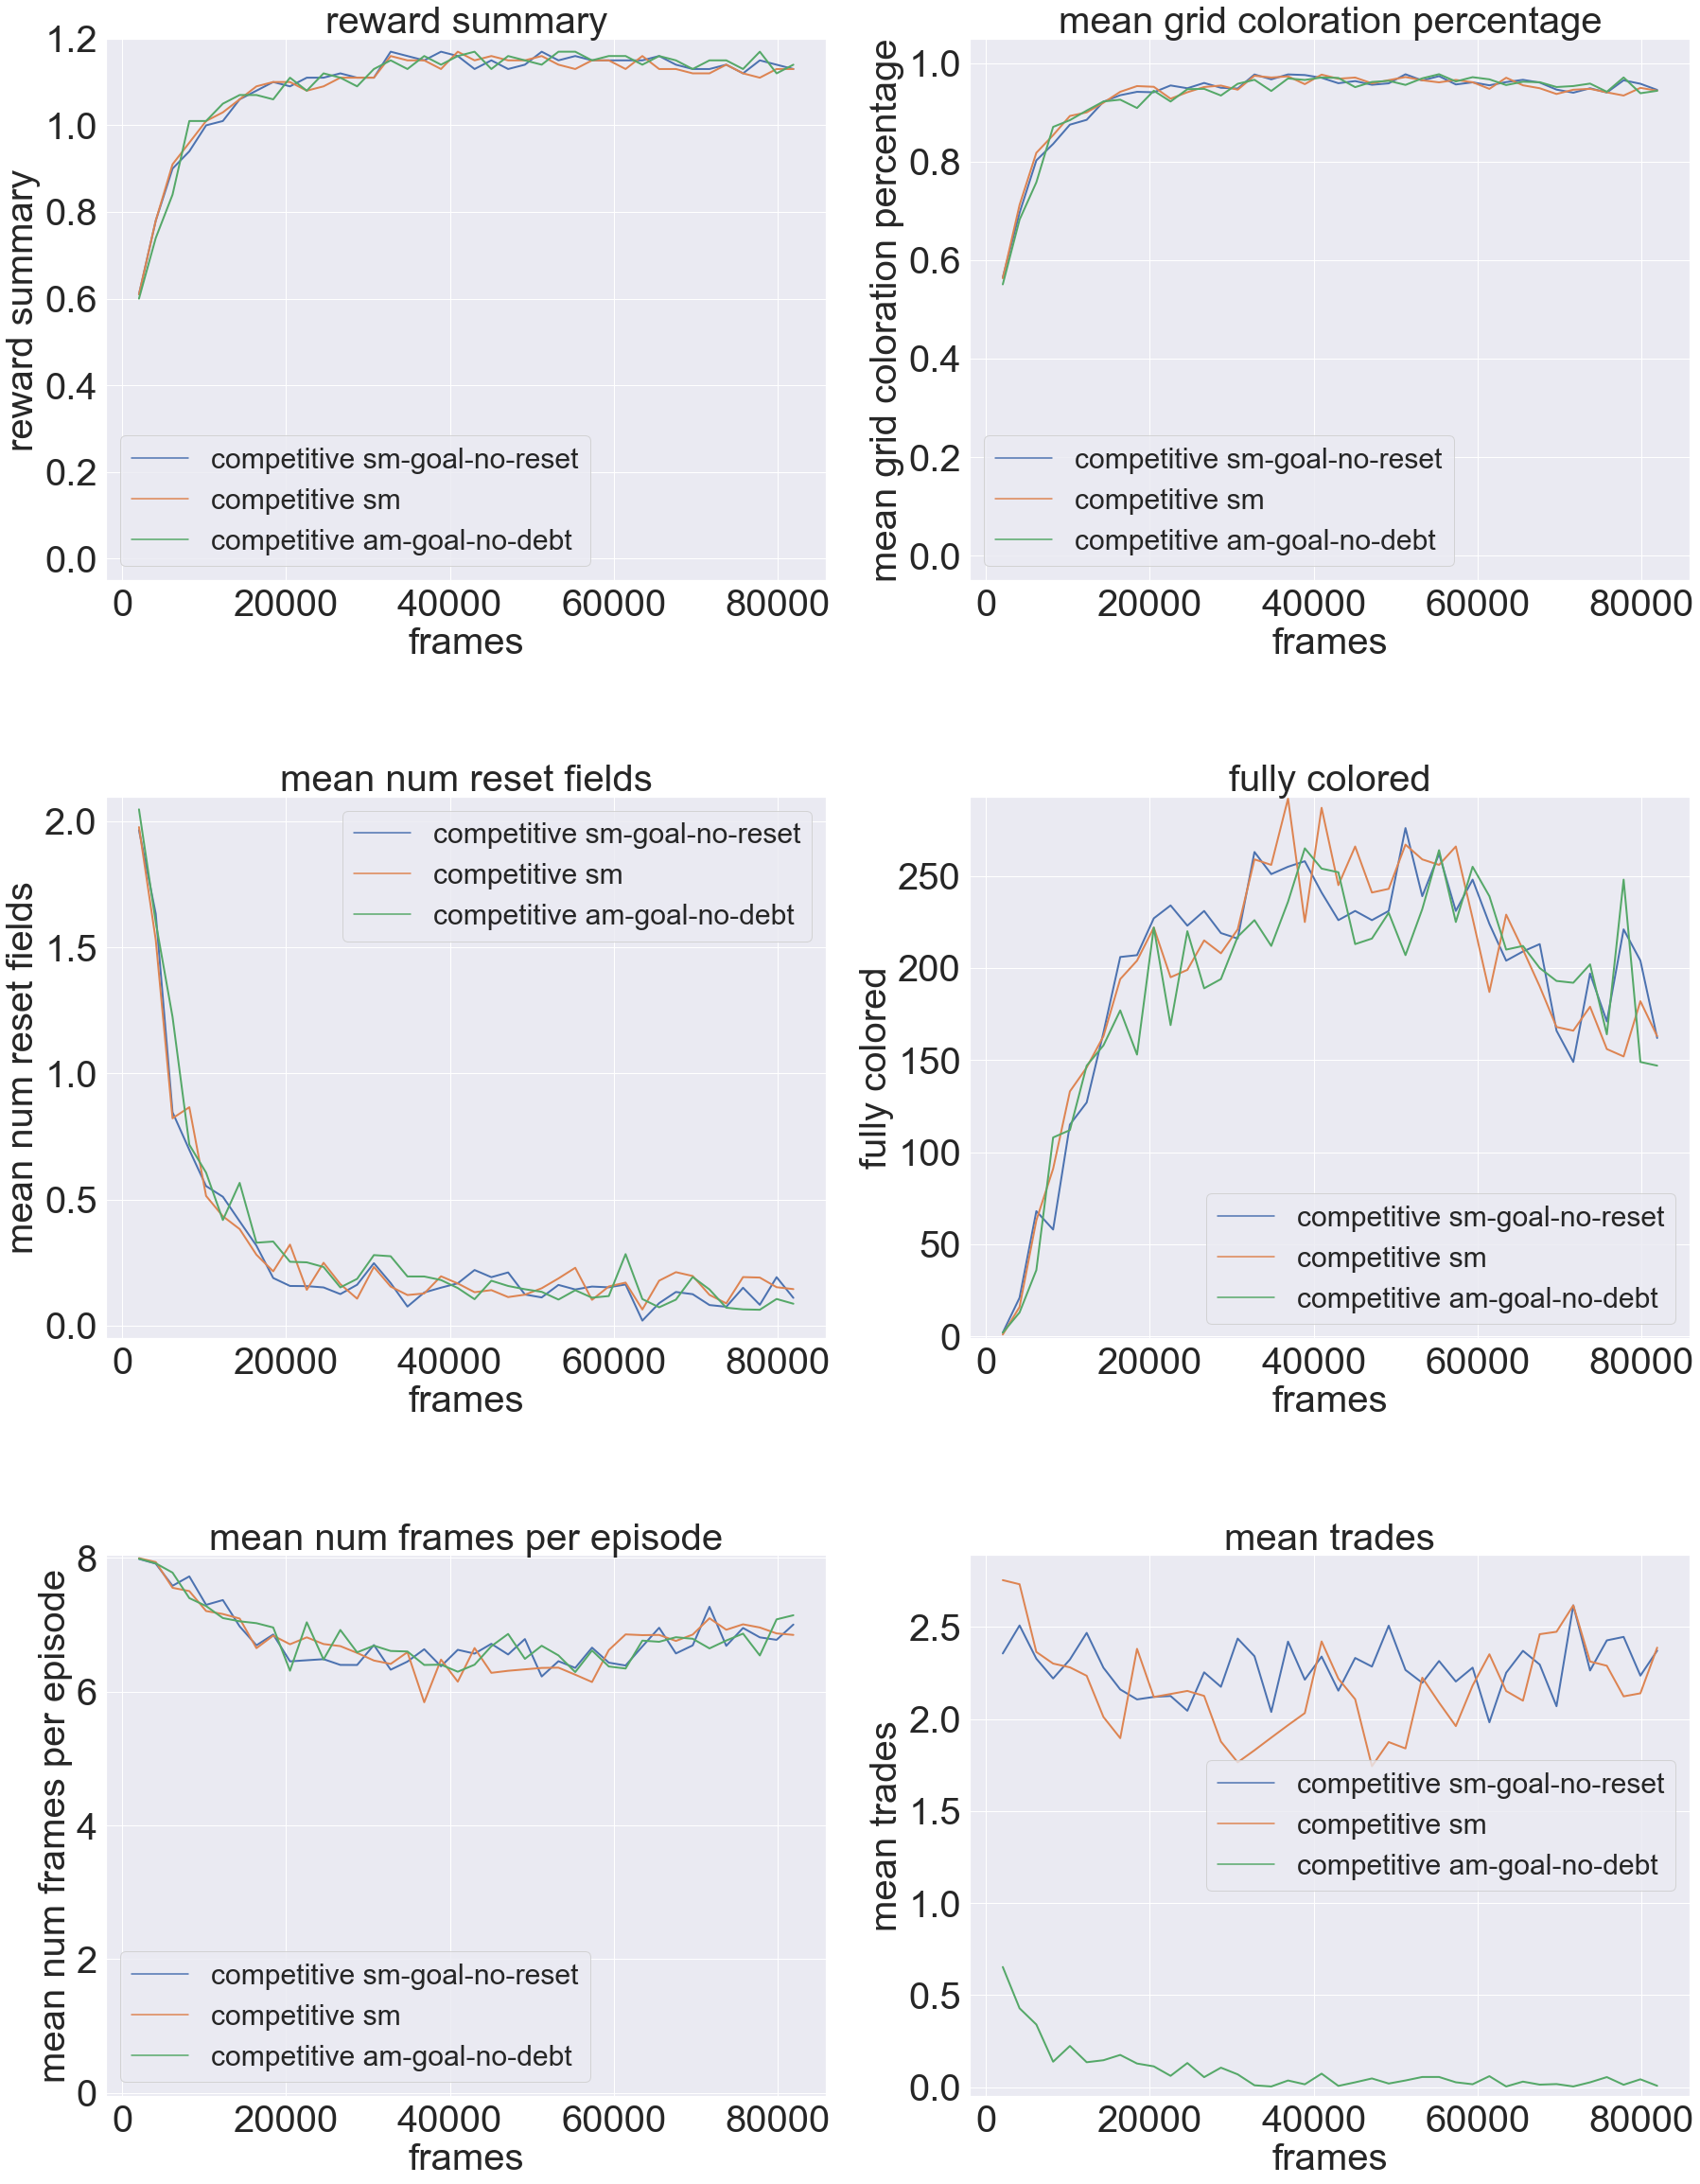
\includegraphics[width=1\textwidth]{AX-easy-2-dqn-comp.png}\\
    \caption[Training Details of Top DQN Competitive Executions]{Top competitive score details of two DQN agents}\label{fig:ax-easy-2-dqn-comp}
\end{figure}
\vfill
\clearpage

\subsection{Difficult Environment}
An example to run a training process in a seven by seven environment is shown below.

\begin{lstlisting}[float=htp,language=bash, escapeinside={//@}{@//},xleftmargin=3ex,xrightmargin=1ex]
$ python -m scripts.train 
    --algo dqn 
    --model dqn-difficult
    --agents 3
    --target-update 10000 
    --replay-size 700000 
    --epsilon-decay 20000
    --grid-size 7 
    --max-steps 20 
    --frames-per-proc 256
    --frames 200000
\end{lstlisting}

\newpage
\vfill
\begin{figure}
    \centering
    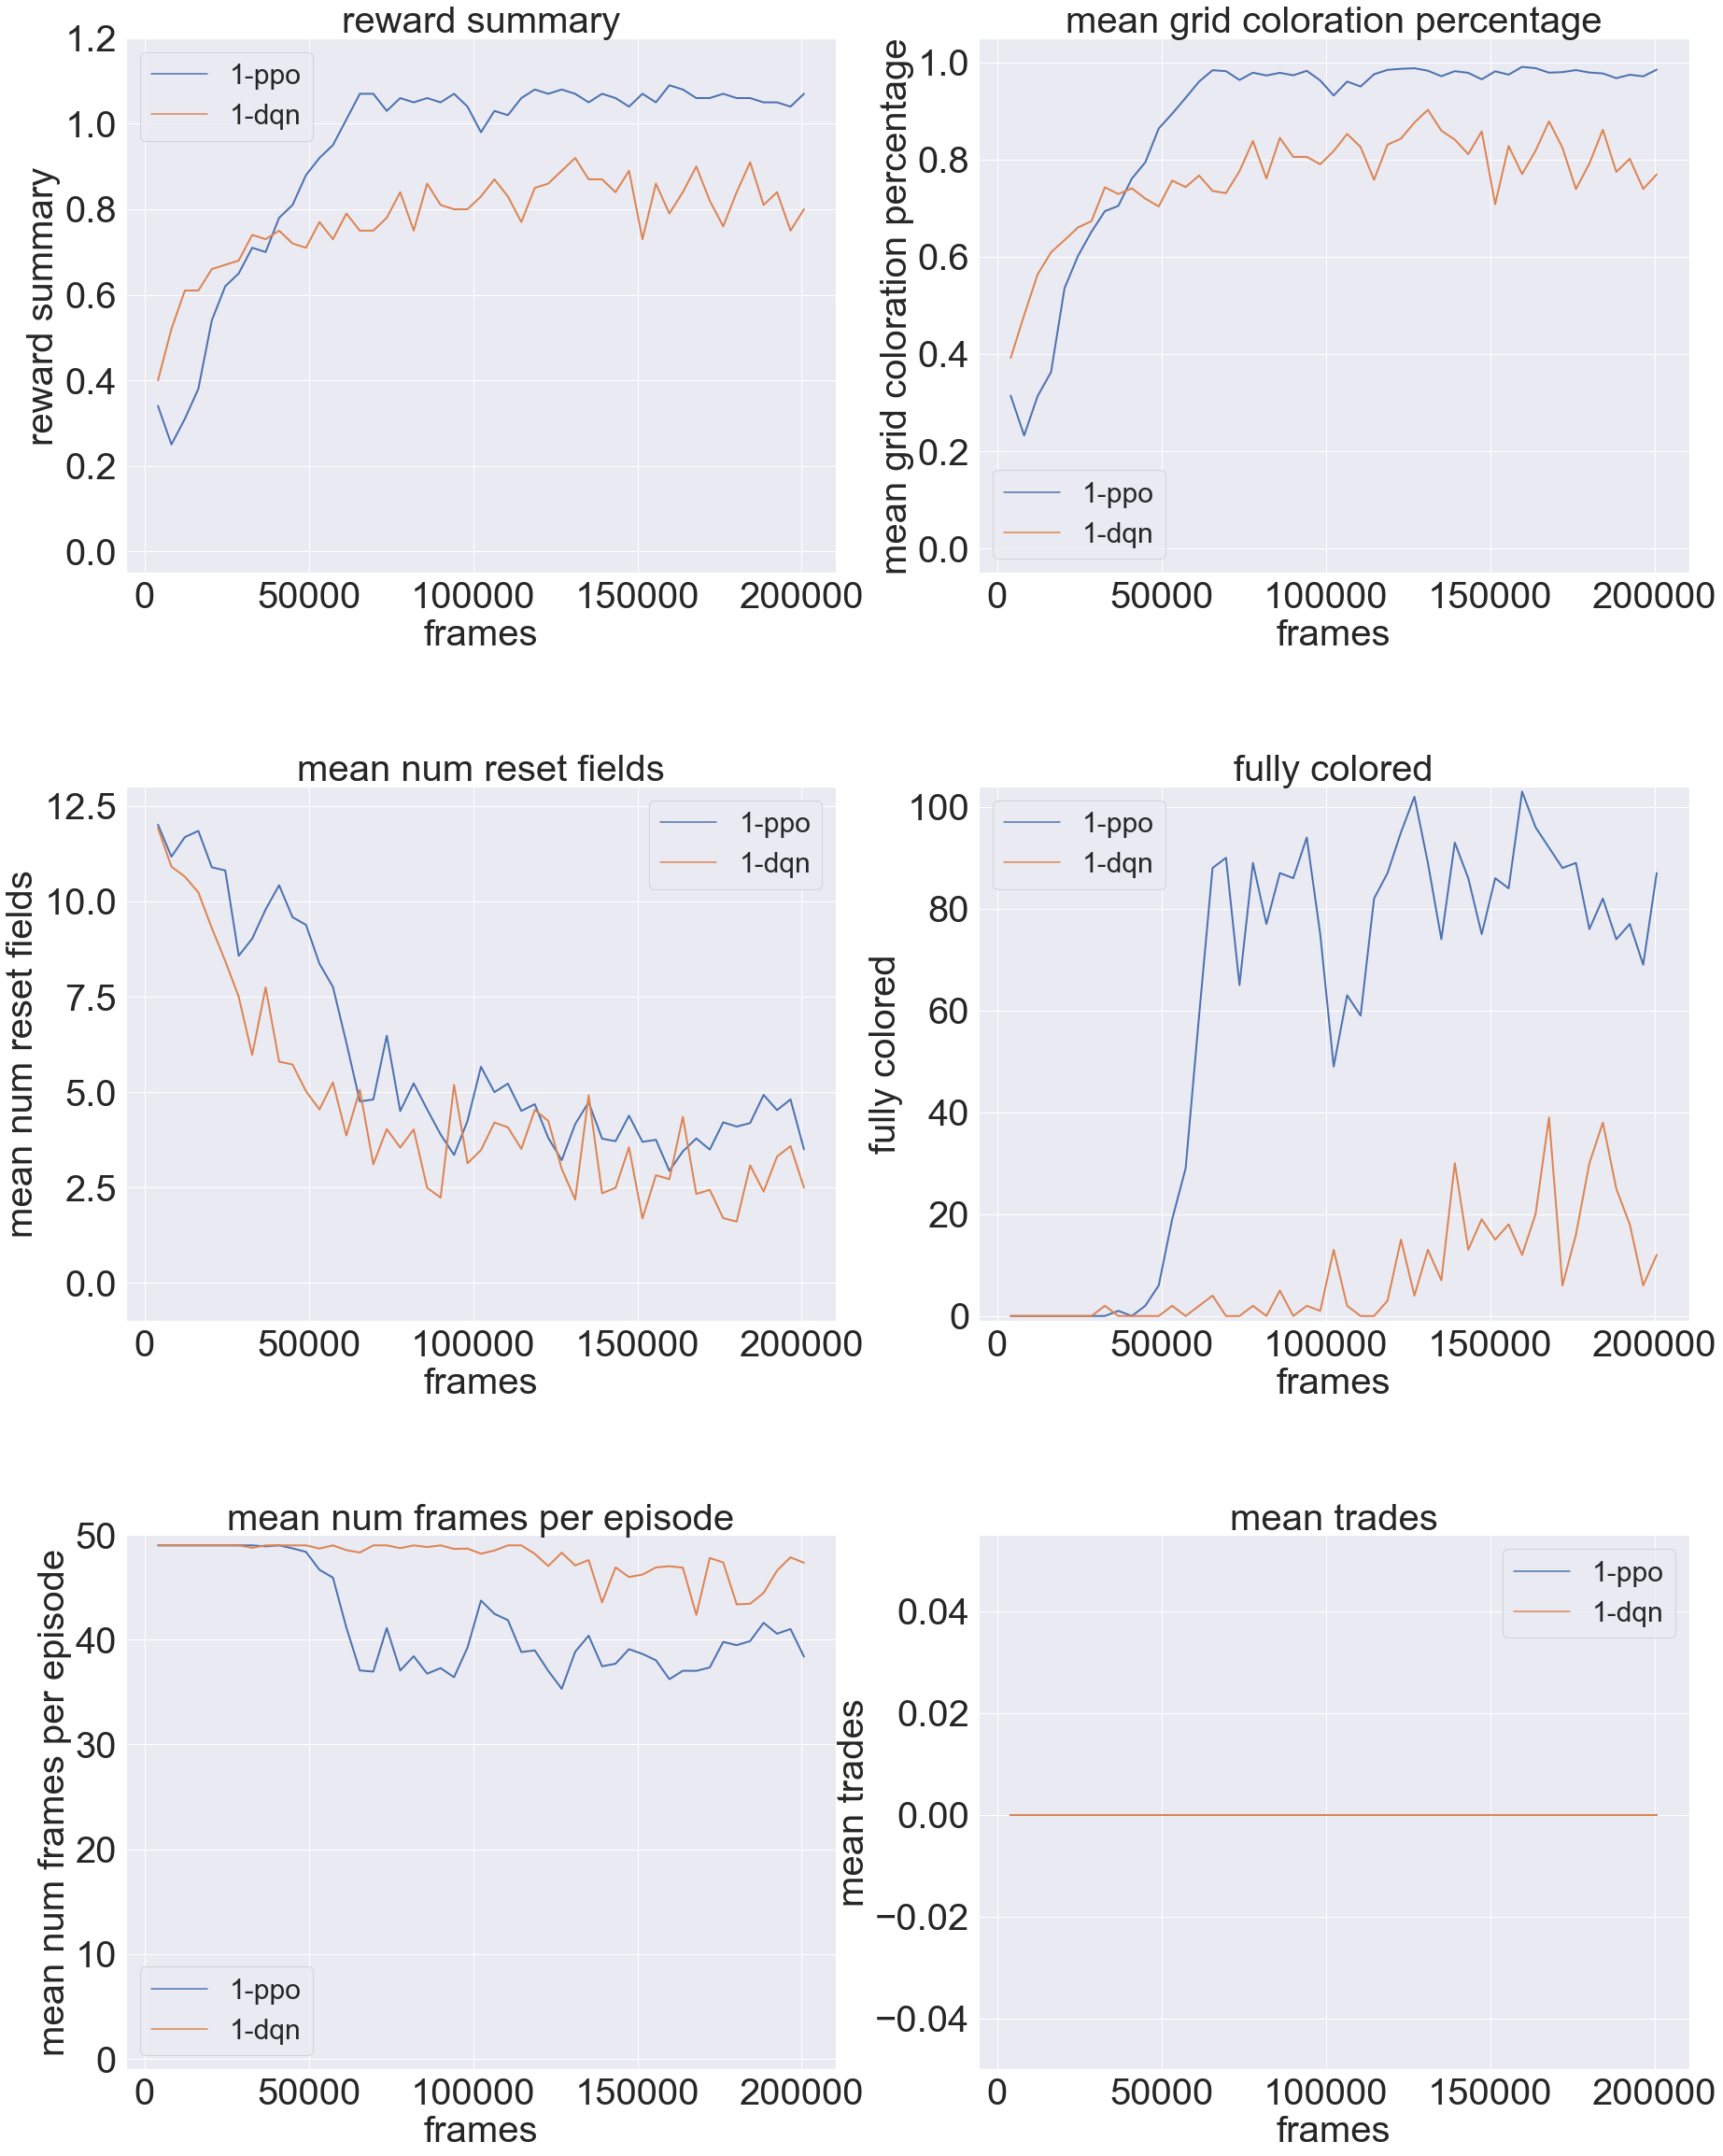
\includegraphics[width=1\textwidth]{AX-hard-1.png}\\
    \caption[PPO and DQN Training Details with One Agent in a 7x7 Environment]{Details of the training  in a 7x7 Environment with one agent using PPO and DQN}\label{fig:ax-hard-1}
\end{figure}
\vfill
\clearpage


\newpage
\vfill
\begin{figure}
    \centering
    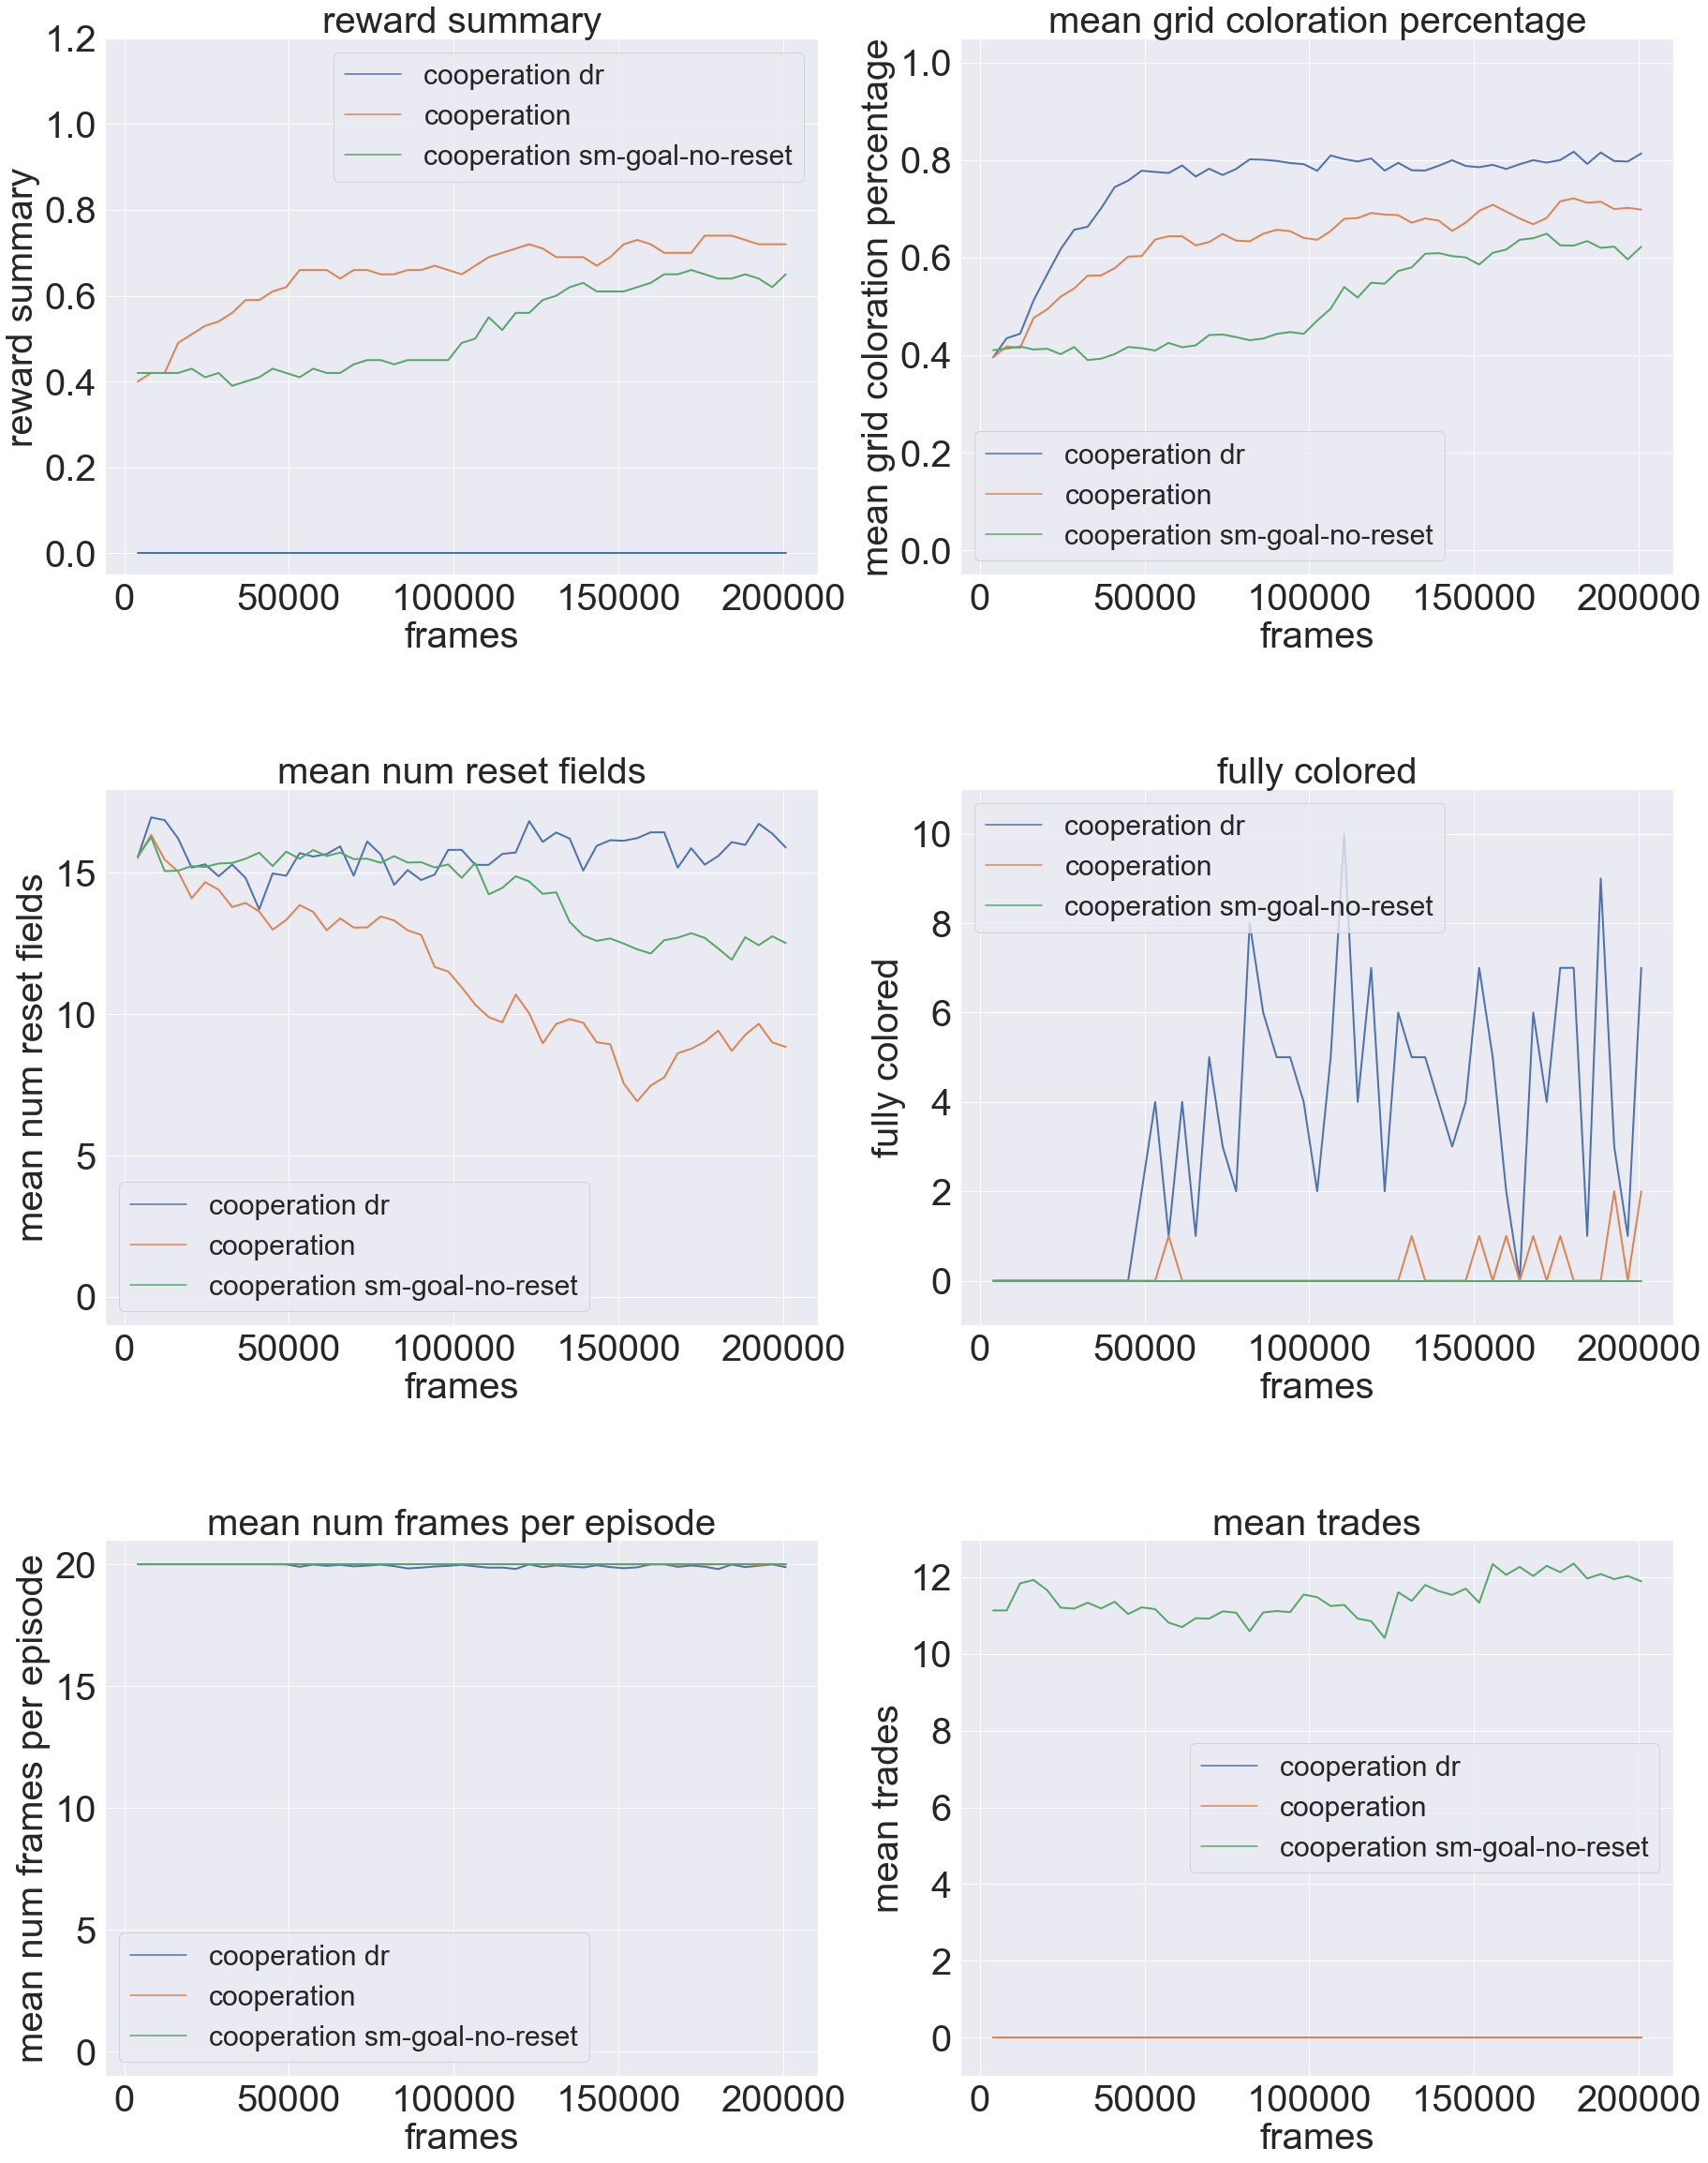
\includegraphics[width=1\textwidth]{AX-hard-3-ppo-coop.png}\\
    \caption[Training Details of Top PPO Cooperation Executions in a 7x7 Environment]{Top cooperation score details of three PPO agents in a 7x7 Environment}\label{fig:ax-hard-2-ppo-coop}
\end{figure}
\vfill
\clearpage


\newpage
\vfill
\begin{figure}
    \centering
    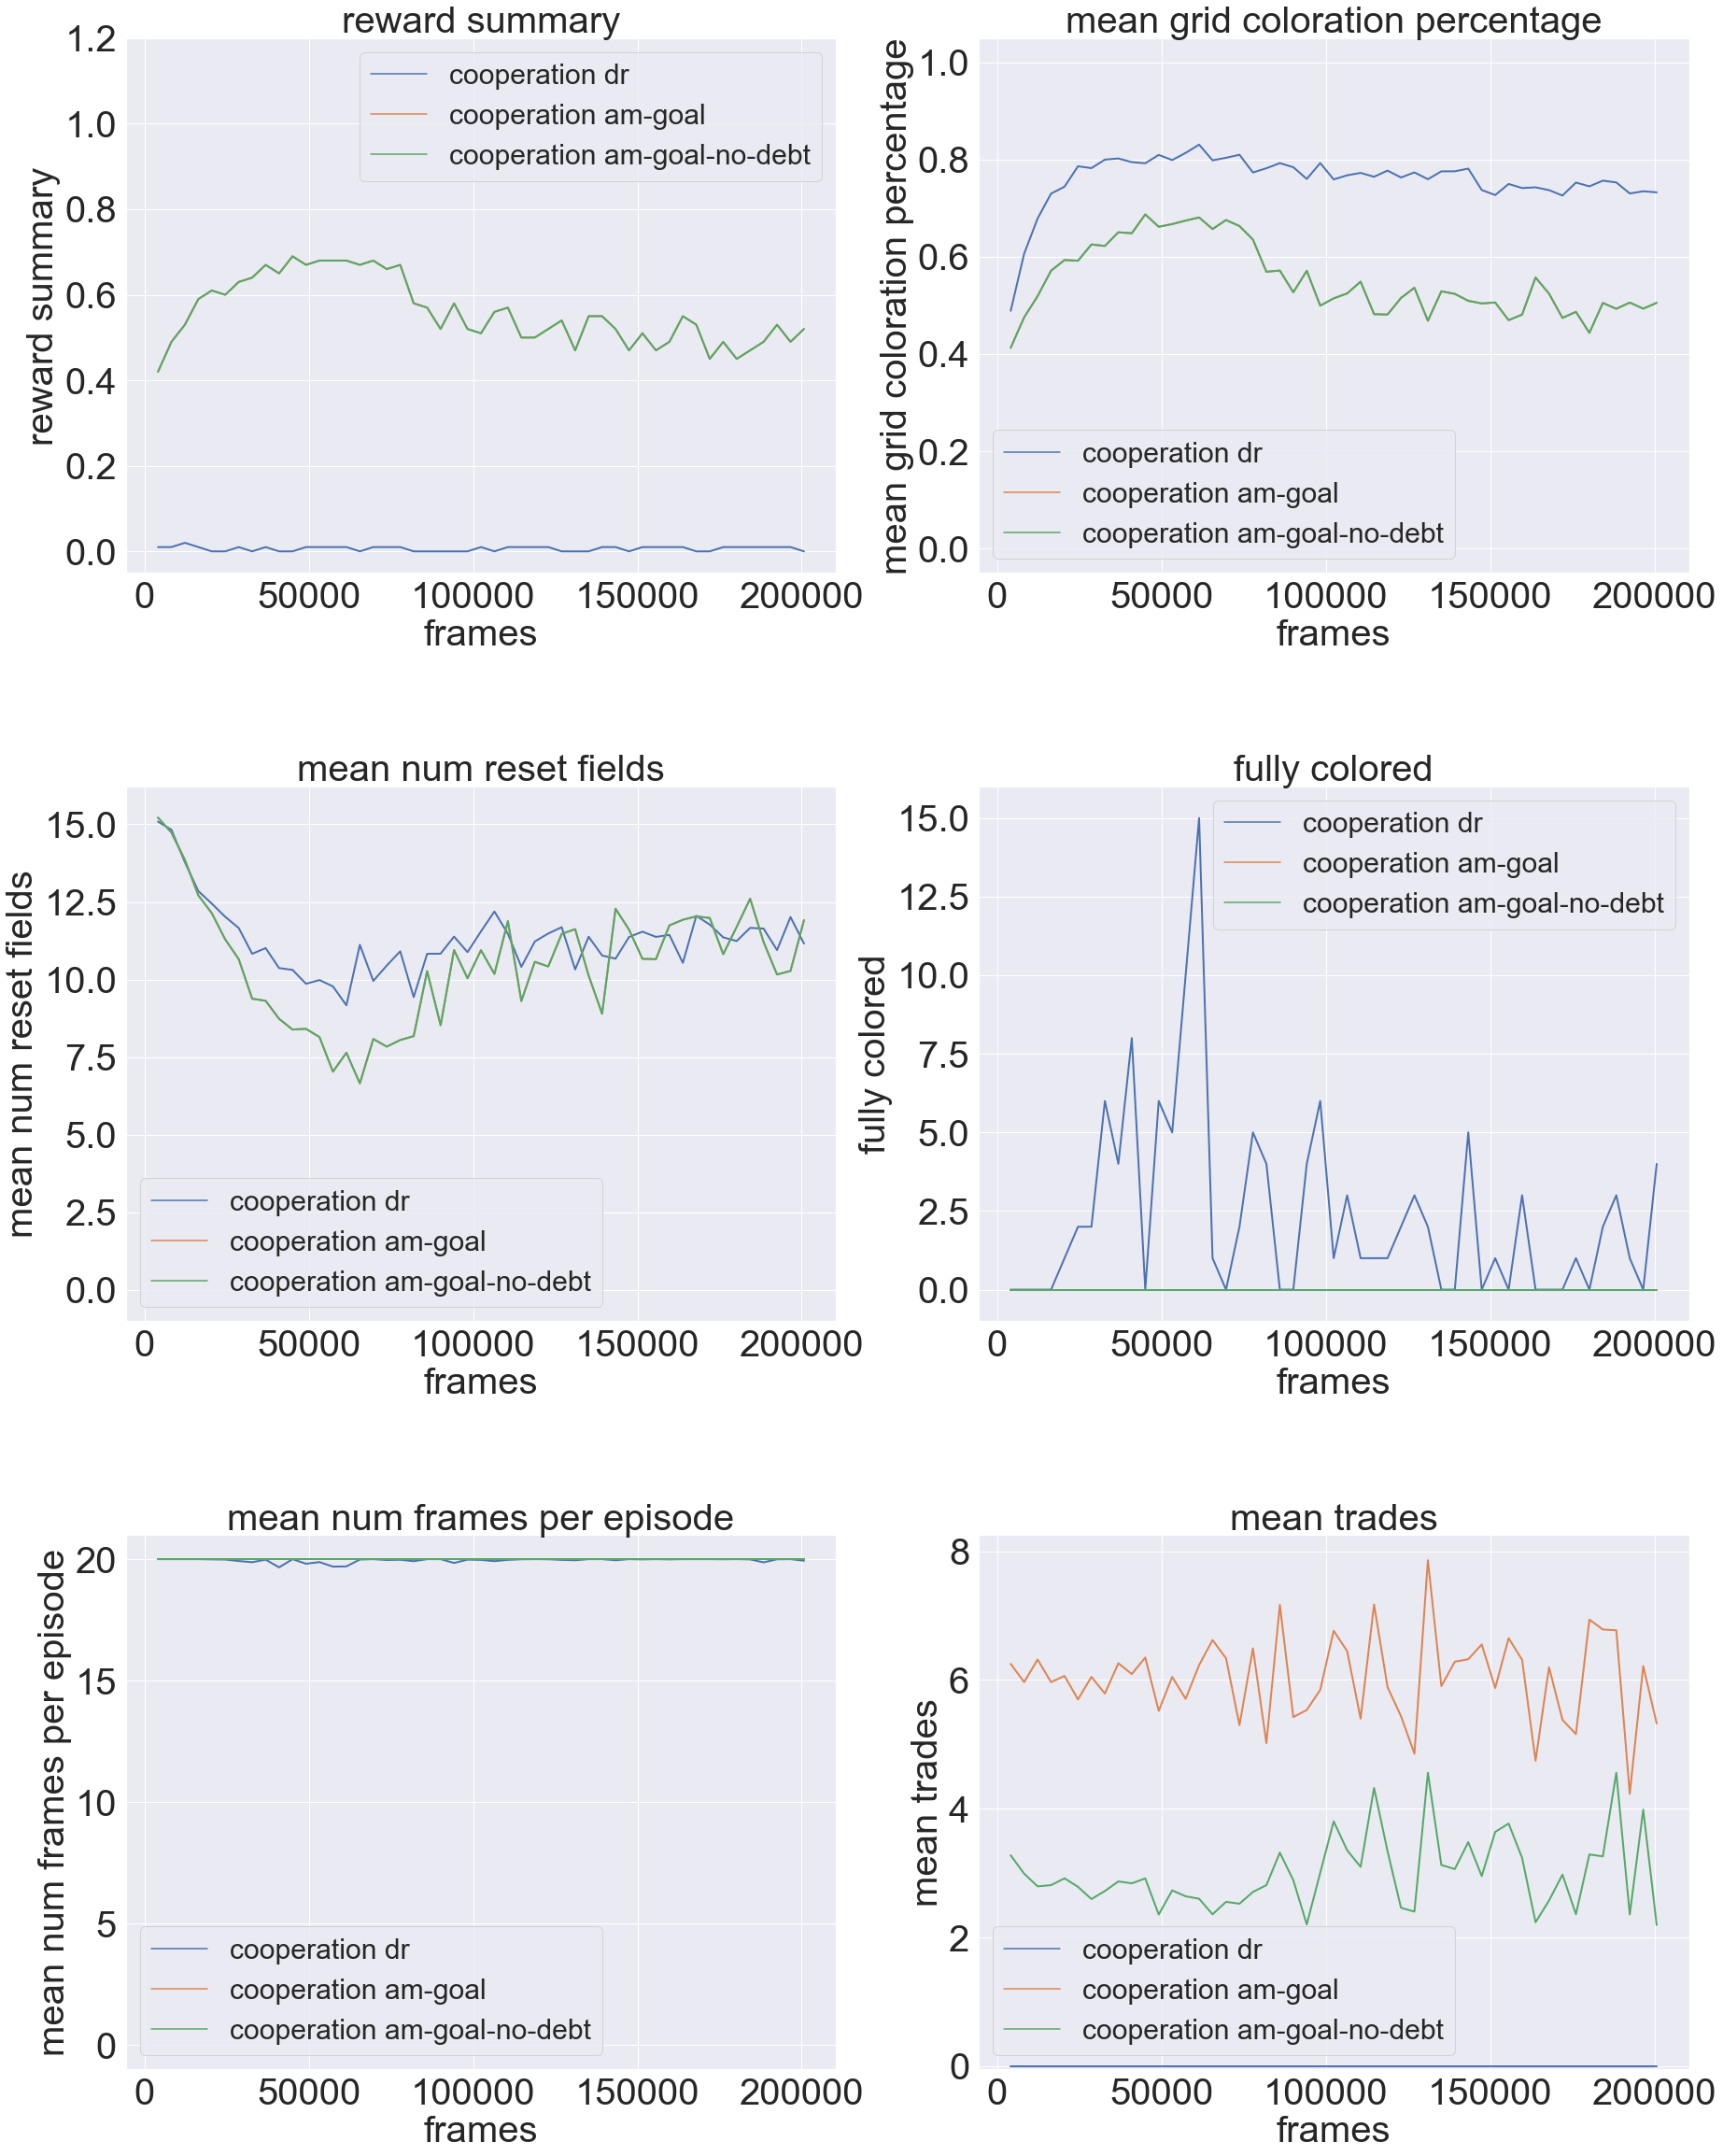
\includegraphics[width=1\textwidth]{AX-hard-3-dqn-coop.png}\\
    \caption[Training Details of Top DQN Cooperation Executions in a 7x7 Environment]{Top cooperation score details of three DQN agents in a 7x7 Environment}\label{fig:ax-hard-2-dqn-coop}
\end{figure}
\vfill
\clearpage


\newpage
\vfill
\begin{figure}
    \centering
    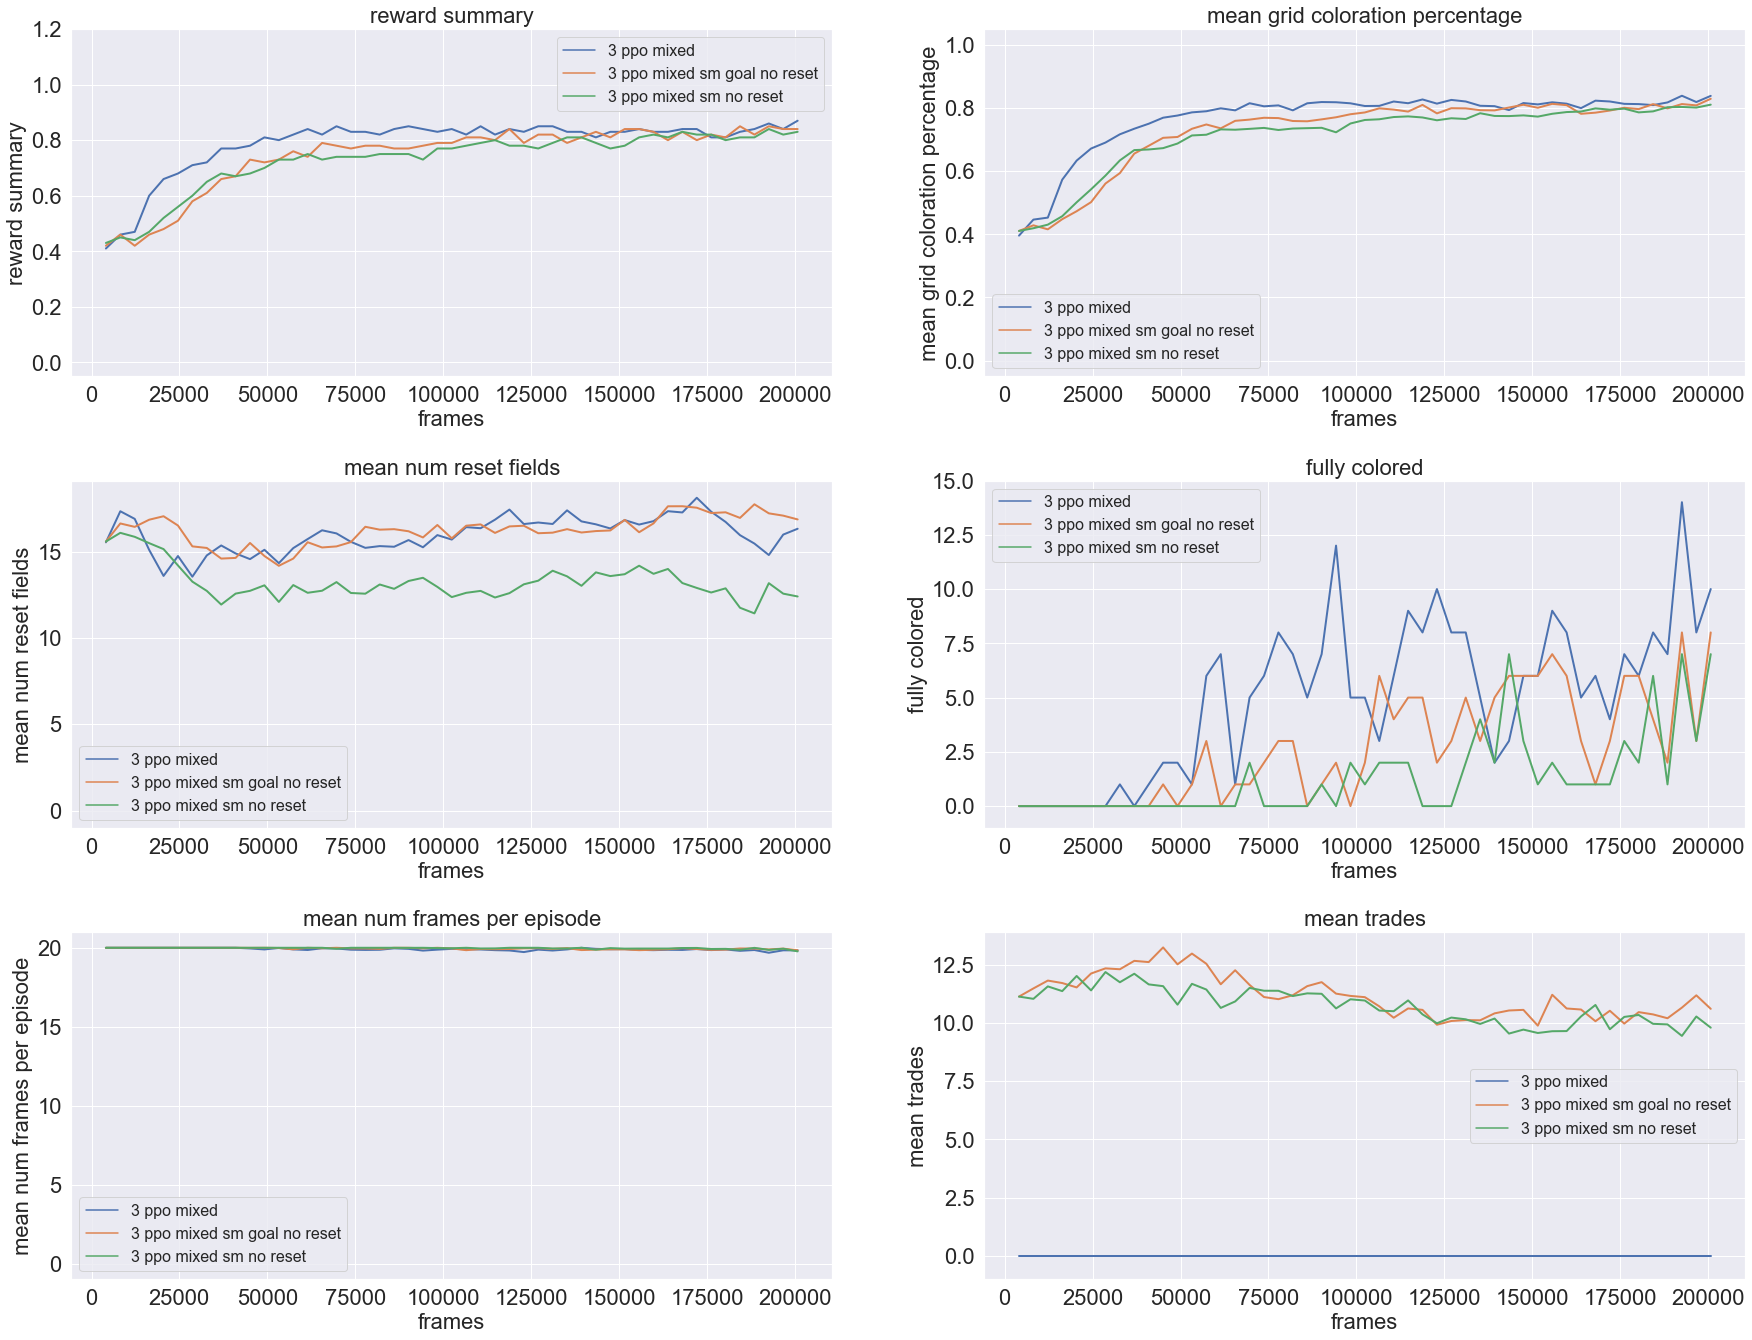
\includegraphics[width=1\textwidth]{AX-hard-3-ppo-mixed.png}\\
    \caption[Training Details of Top PPO Mixed-Motive Executions in a 7x7 Environment]{Top mixed-motive score details of three PPO agents in a 7x7 Environment}\label{fig:ax-hard-2-ppo-mixed}
\end{figure}
\vfill
\clearpage


\newpage
\vfill
\begin{figure}
    \centering
    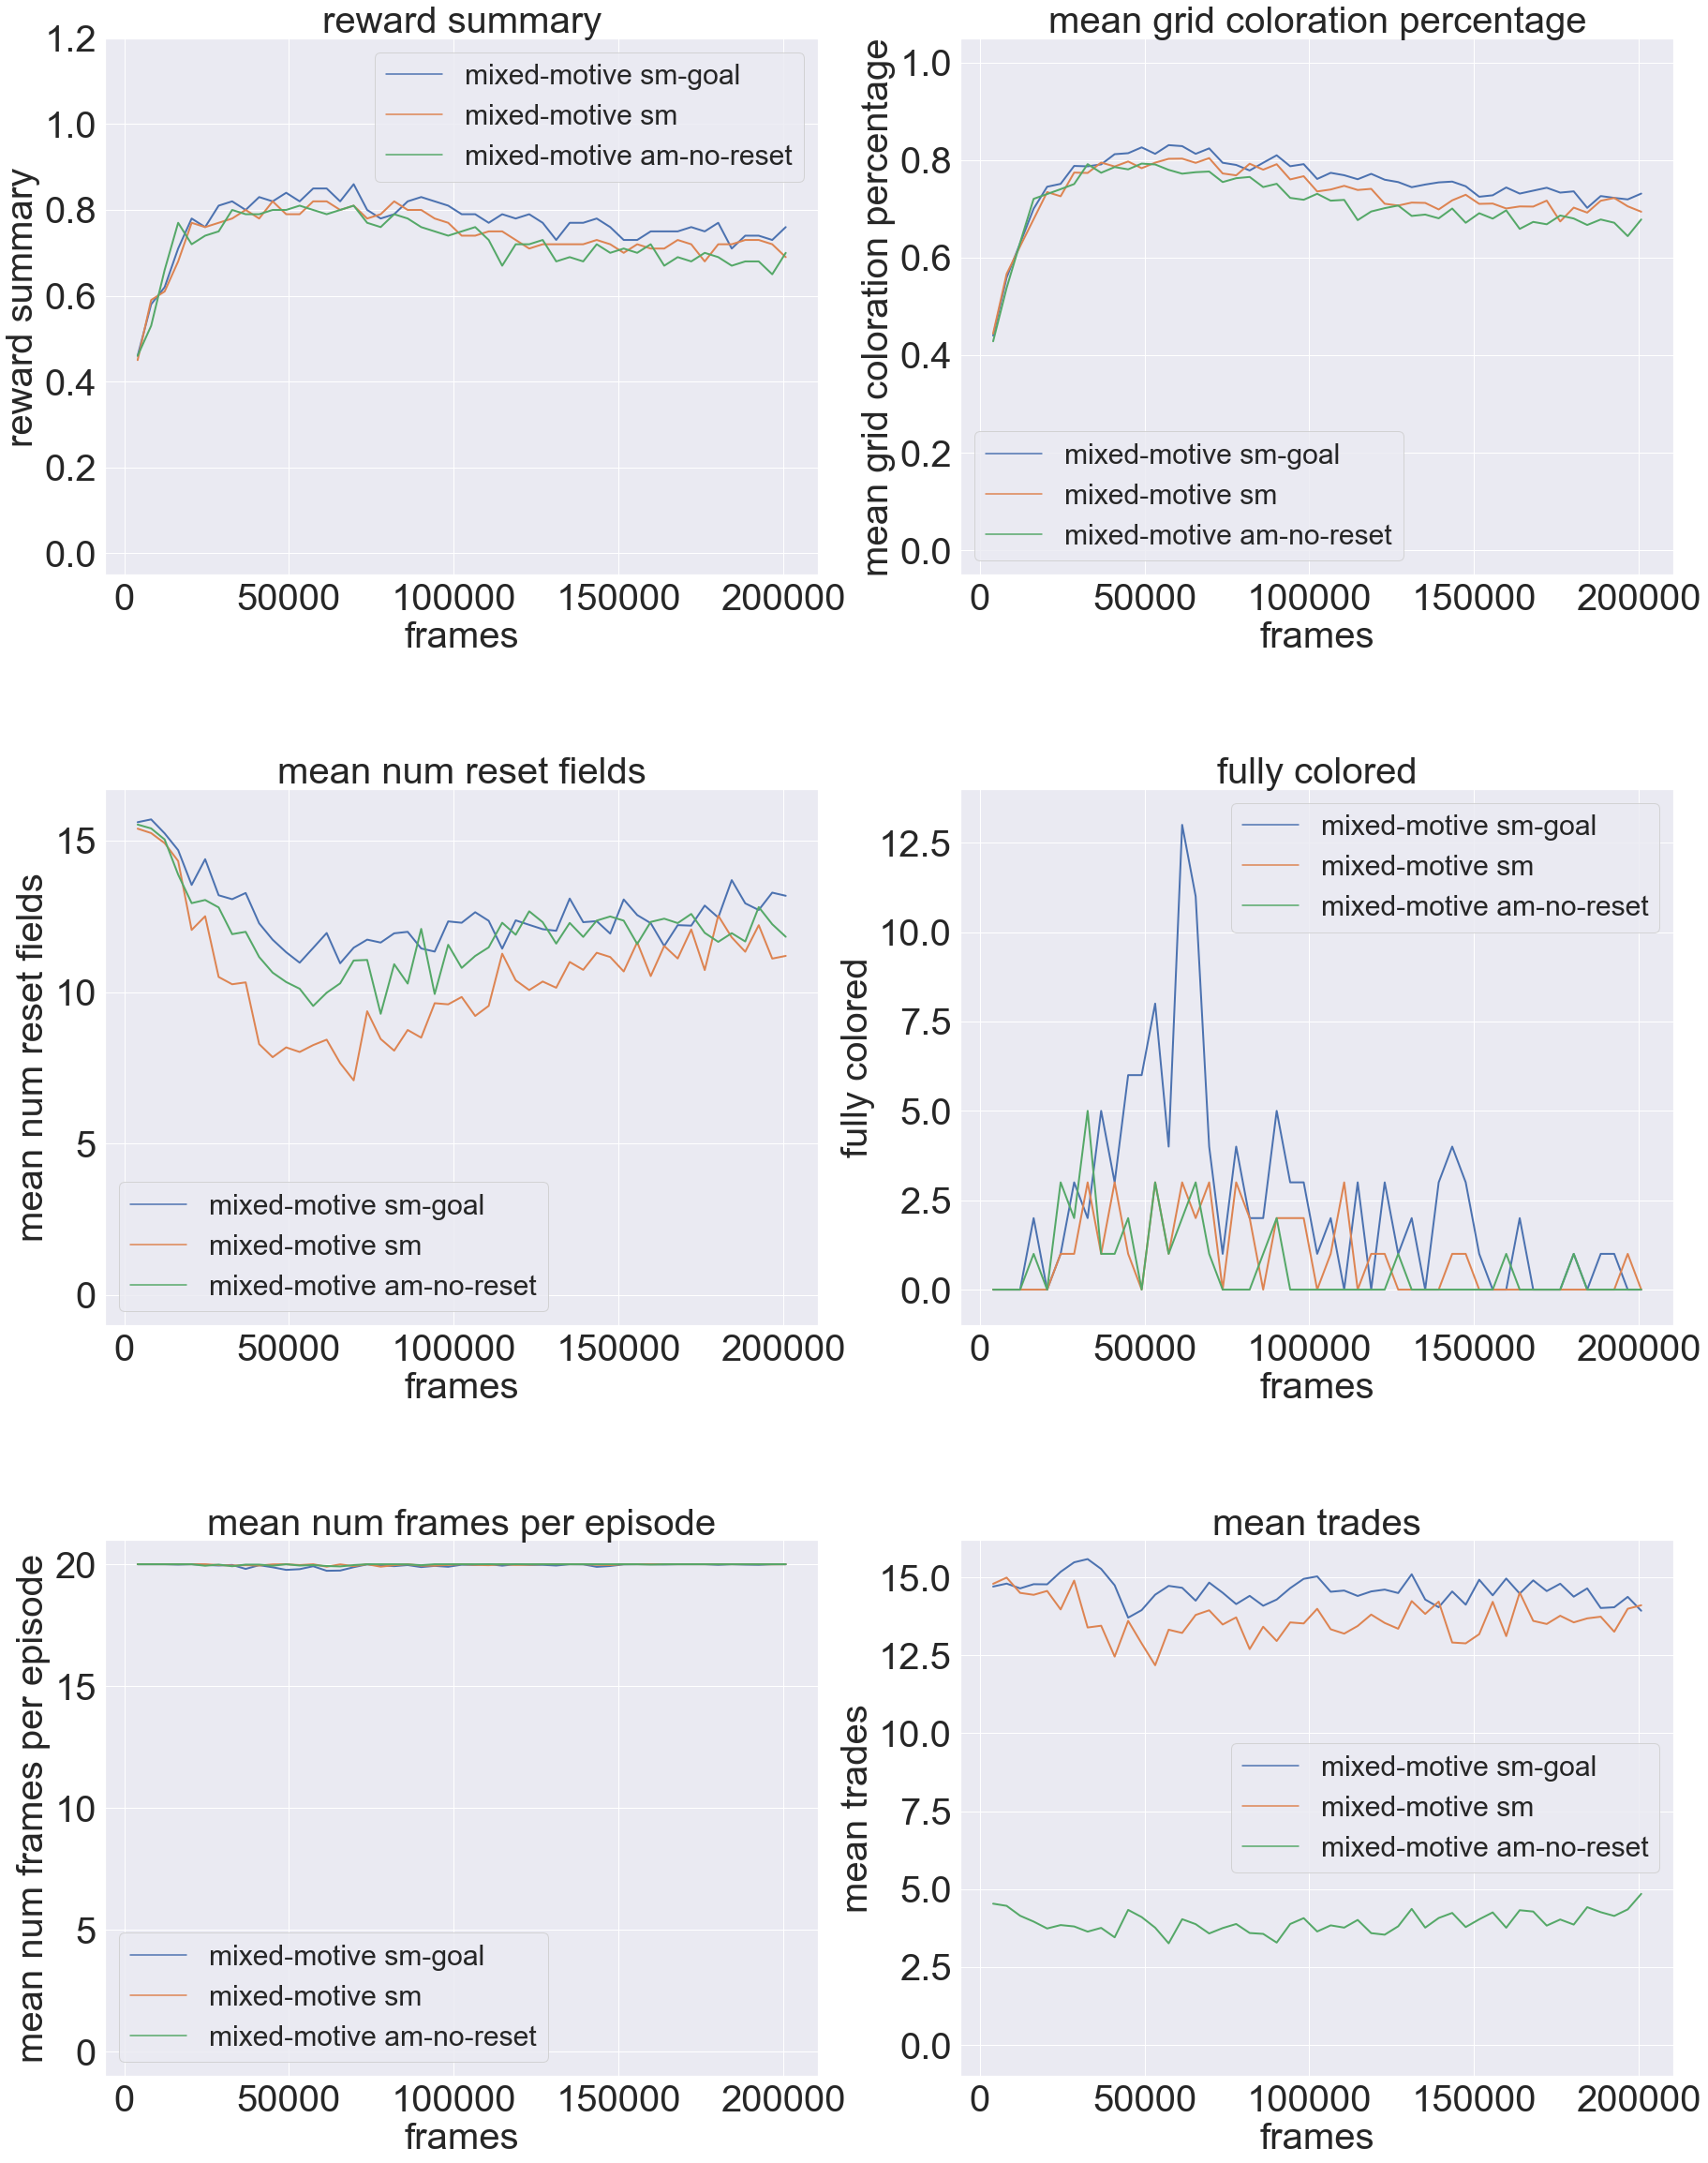
\includegraphics[width=1\textwidth]{AX-hard-3-dqn-mixed.png}\\
    \caption[Training Details of Top DQN Mixed-Motive Executions in a 7x7 Environment]{Top mixed-motive score details of three DQN agents in a 7x7 Environment}\label{fig:ax-hard-2-dqn-mixed}
\end{figure}
\vfill
\clearpage


\newpage
\vfill
\begin{figure}
    \centering
    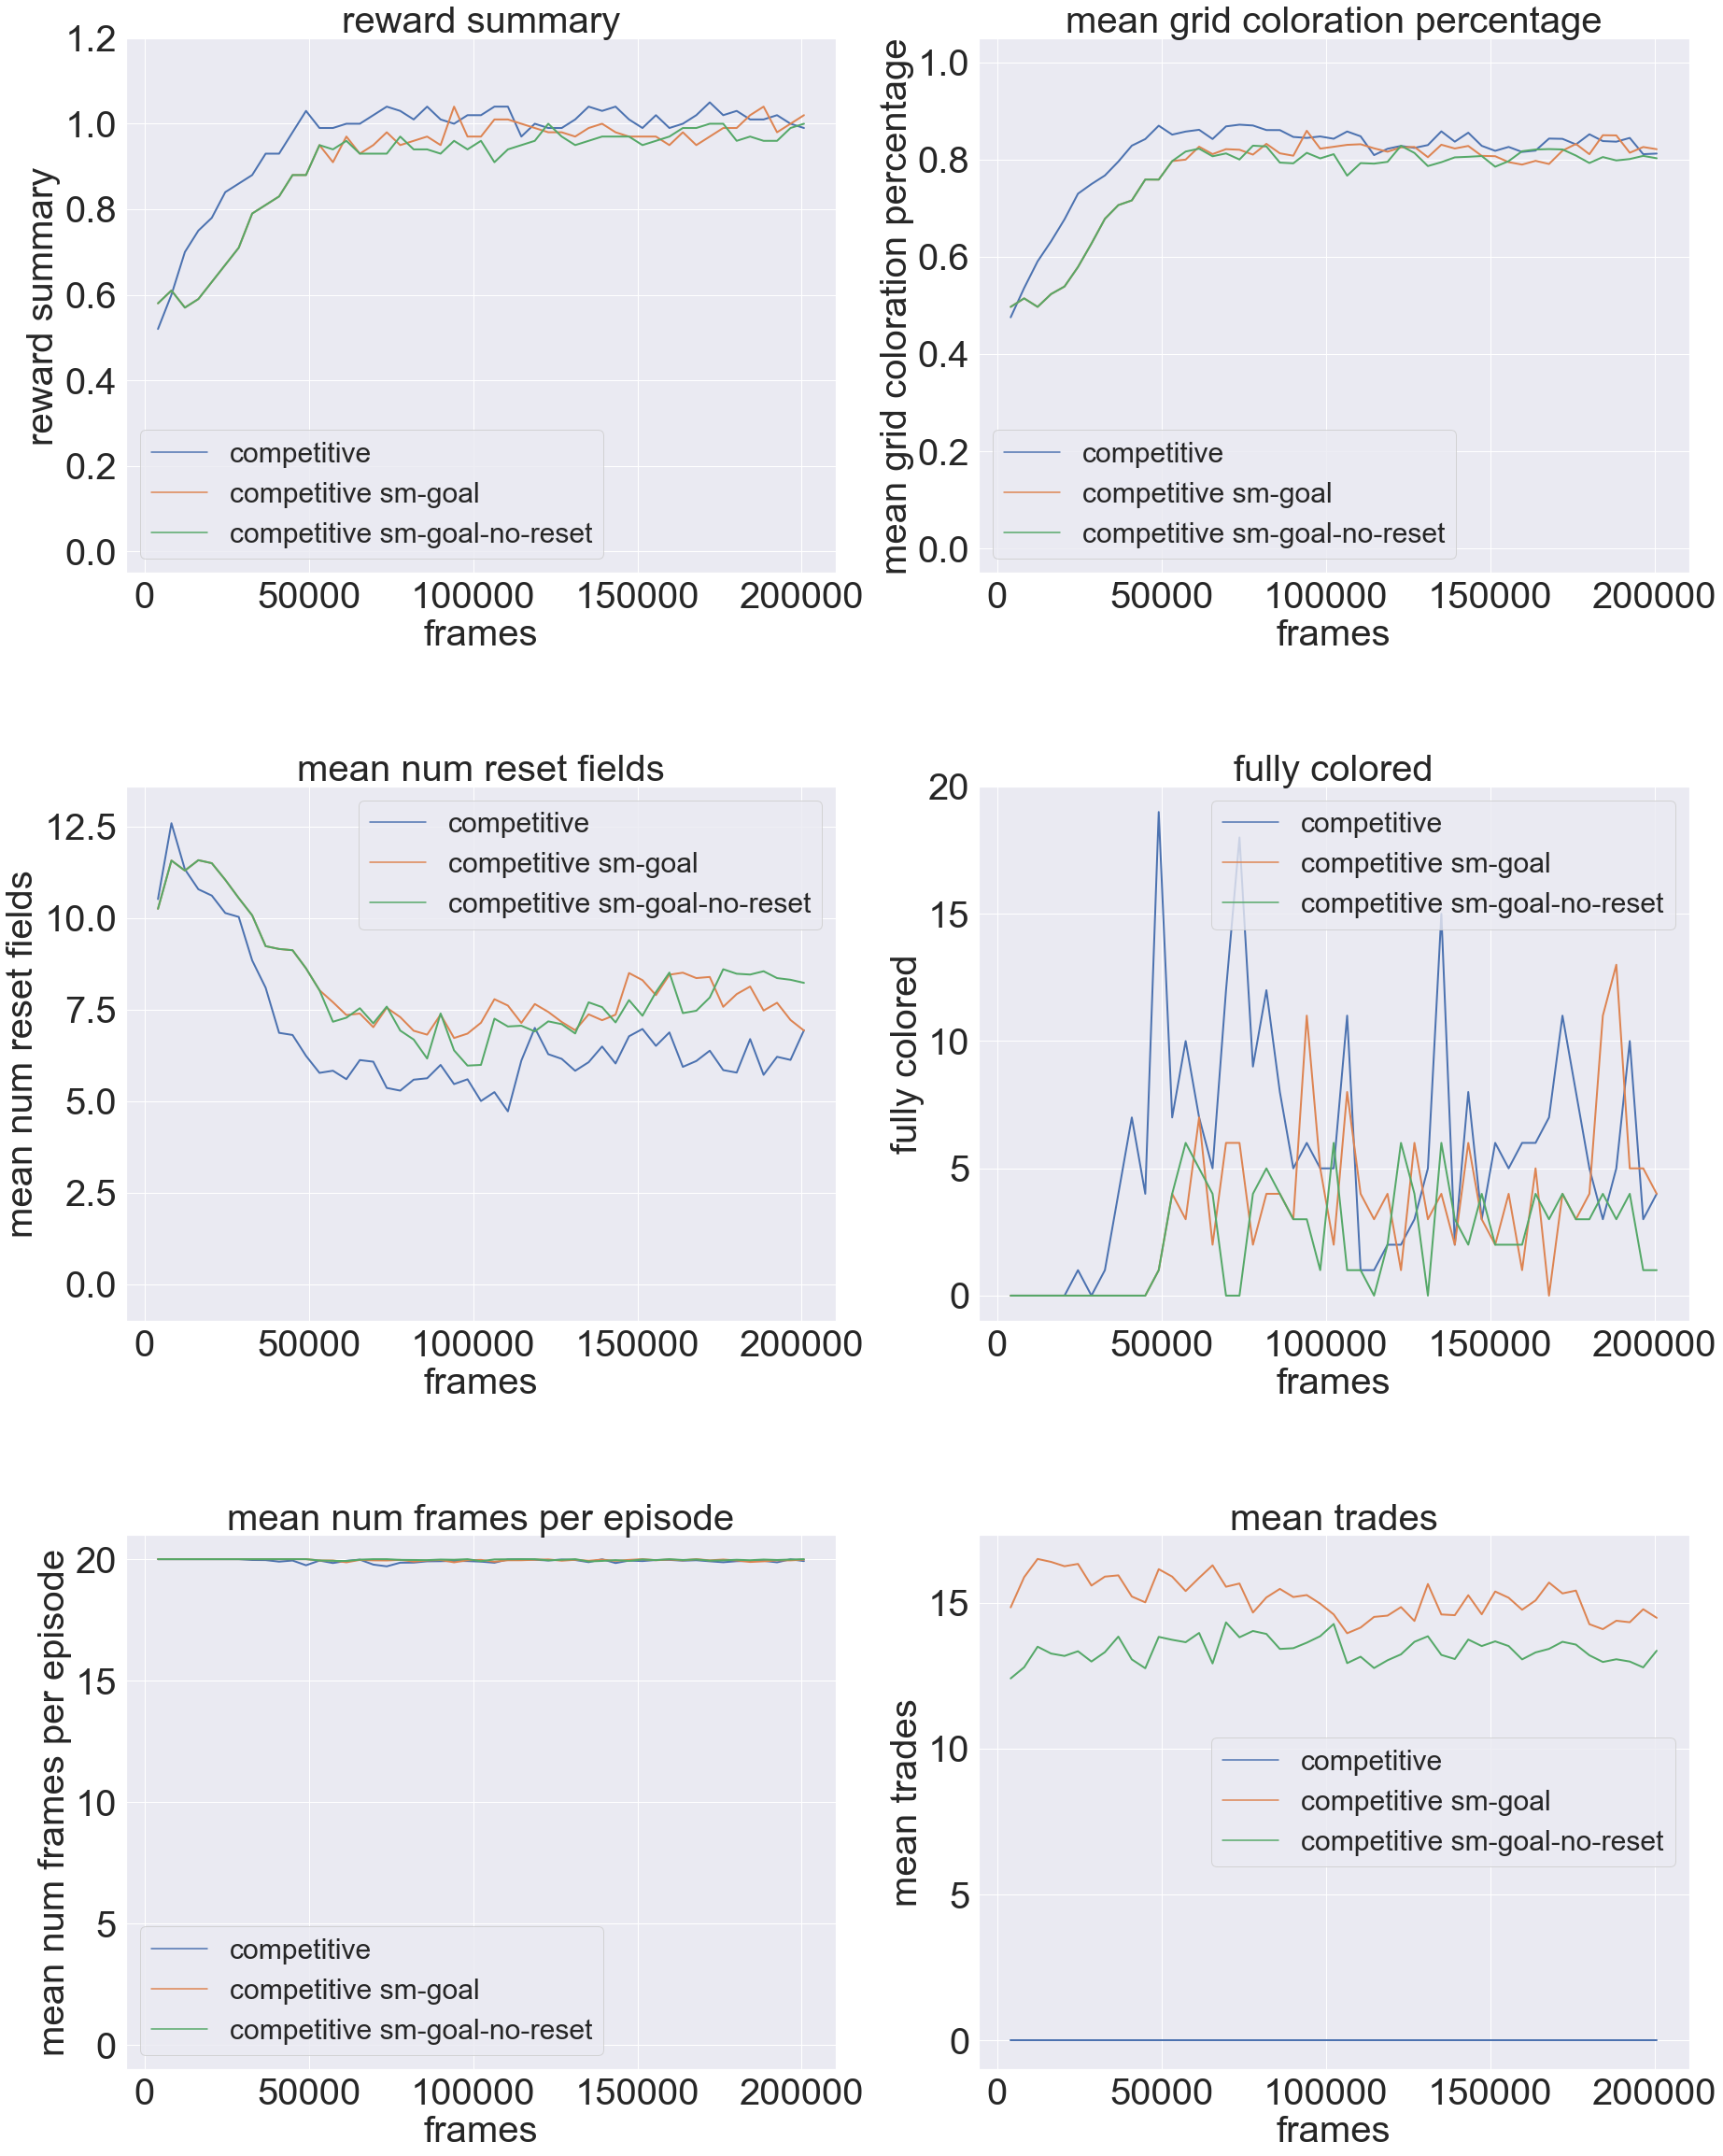
\includegraphics[width=1\textwidth]{AX-hard-3-ppo-comp.png}\\
    \caption[Training Details of Top PPO Competitive Executions in a 7x7 Environment]{Top competitive score details of three PPO agents in a 7x7 Environment}\label{fig:ax-hard-2-ppo-comp}
\end{figure}
\vfill
\clearpage


\newpage
\vfill
\begin{figure}
    \centering
    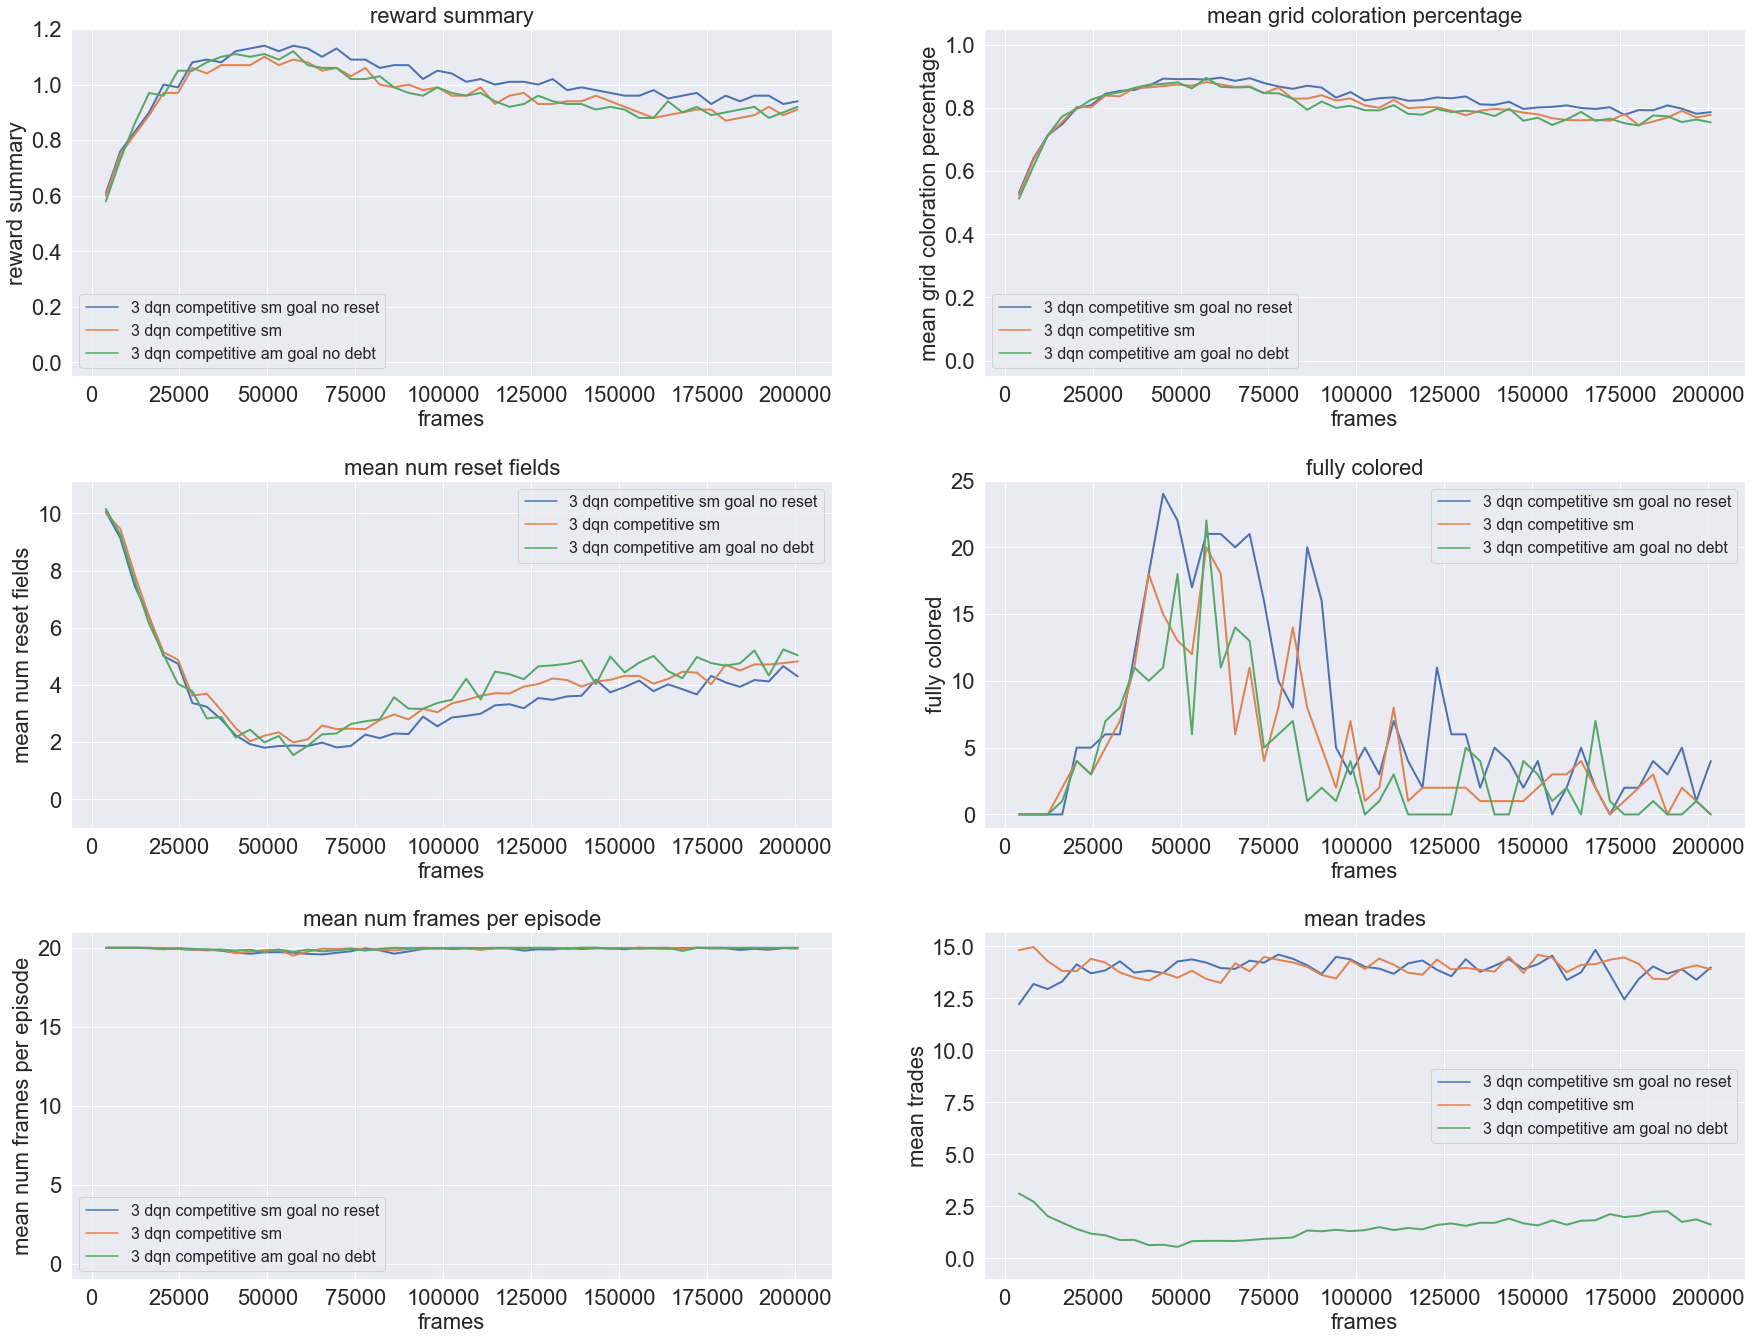
\includegraphics[width=1\textwidth]{AX-hard-3-dqn-comp.png}\\
    \caption[Training Details of Top DQN Competitive Executions in a 7x7 Environment]{Top competitive score details of three DQN agents in a 7x7 Environment}\label{fig:ax-hard-2-dqn-comp}
\end{figure}
\vfill
\clearpage


\subsection{Rooms Environment}
An example to run a training process in a nine by nine room divided environment is shown below.

\begin{lstlisting}[float=htp,language=bash, escapeinside={//@}{@//},xleftmargin=3ex,xrightmargin=1ex]
$ python -m scripts.train 
    --algo ppo 
    --agents 3 
    --model ppo-rooms
    --env FourRooms-Grid-v0 
    --grid-size 9 
    --max-steps 30 
    --frames-per-proc 256 
    --frames 200000 
\end{lstlisting}

\newpage
\vfill
\begin{figure}
    \centering
    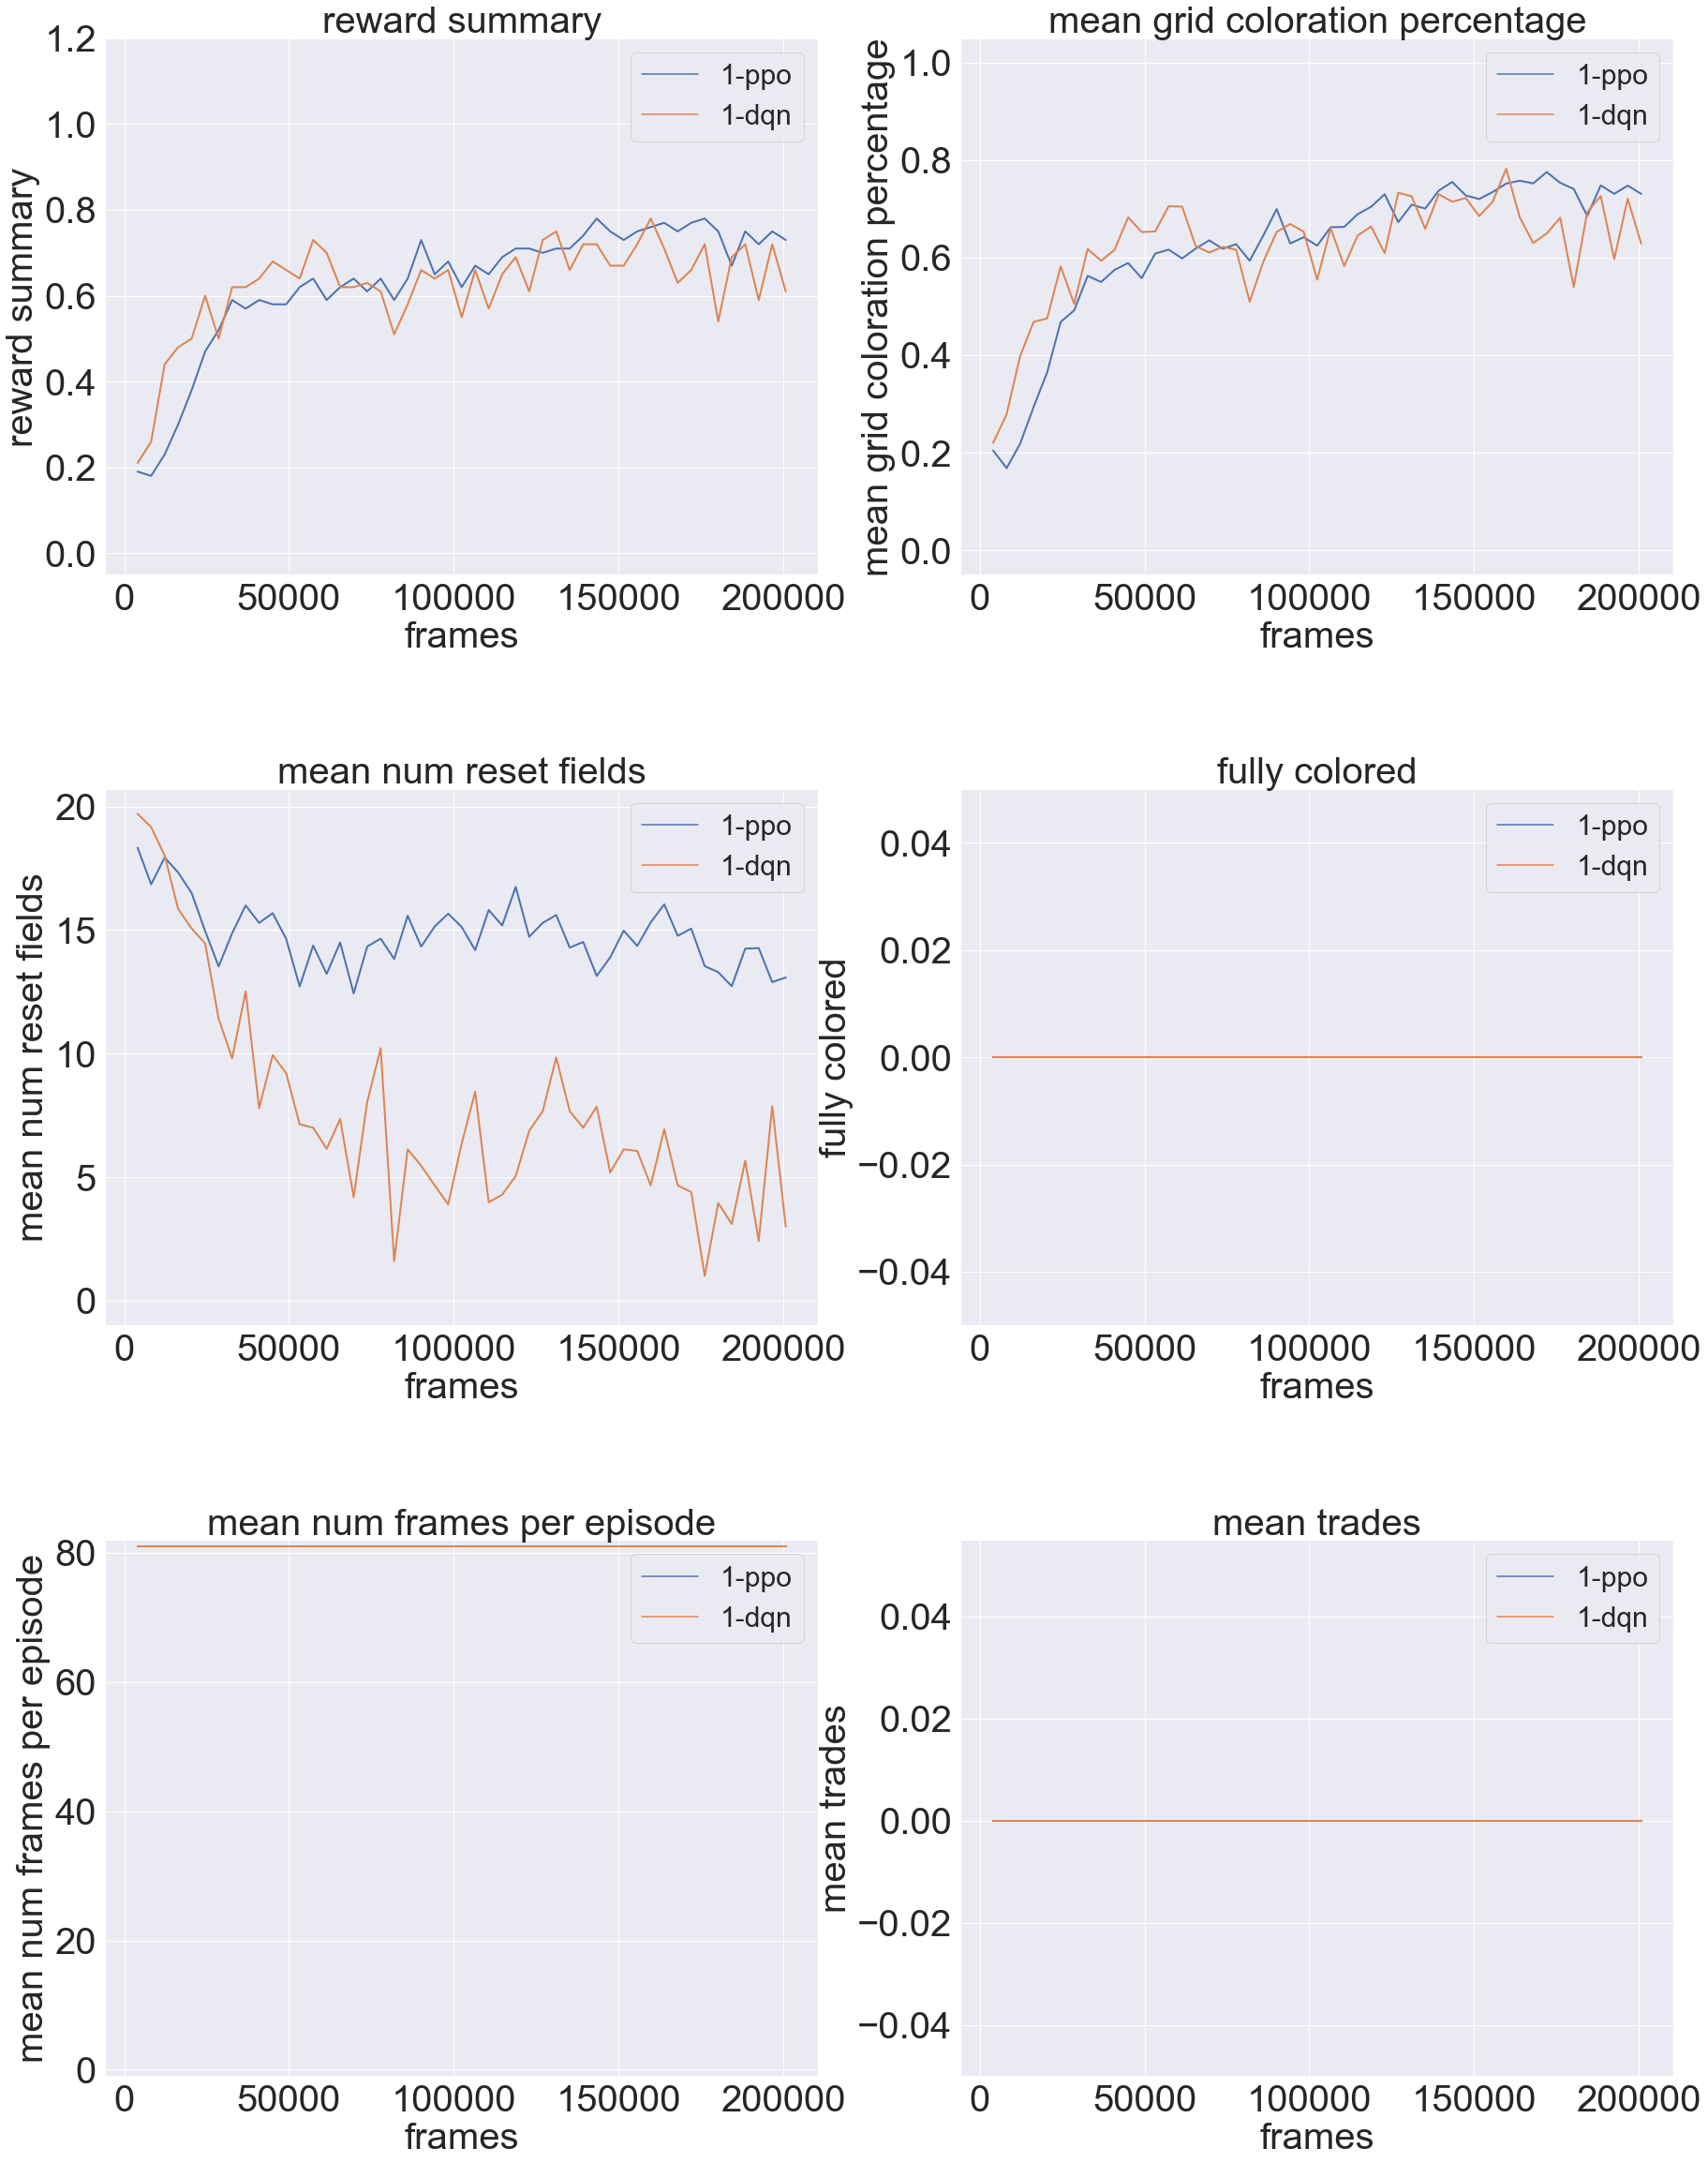
\includegraphics[width=1\textwidth]{AX-rooms-1.png}\\
    \caption[PPO and DQN Training Details with One Agent in a Rooms Environment]{Details of the training  in a 9x9 Rooms Environment with one agent using PPO and DQN}\label{fig:ax-rooms-1}
\end{figure}
\vfill
\clearpage


\newpage
\vfill
\begin{figure}
    \centering
    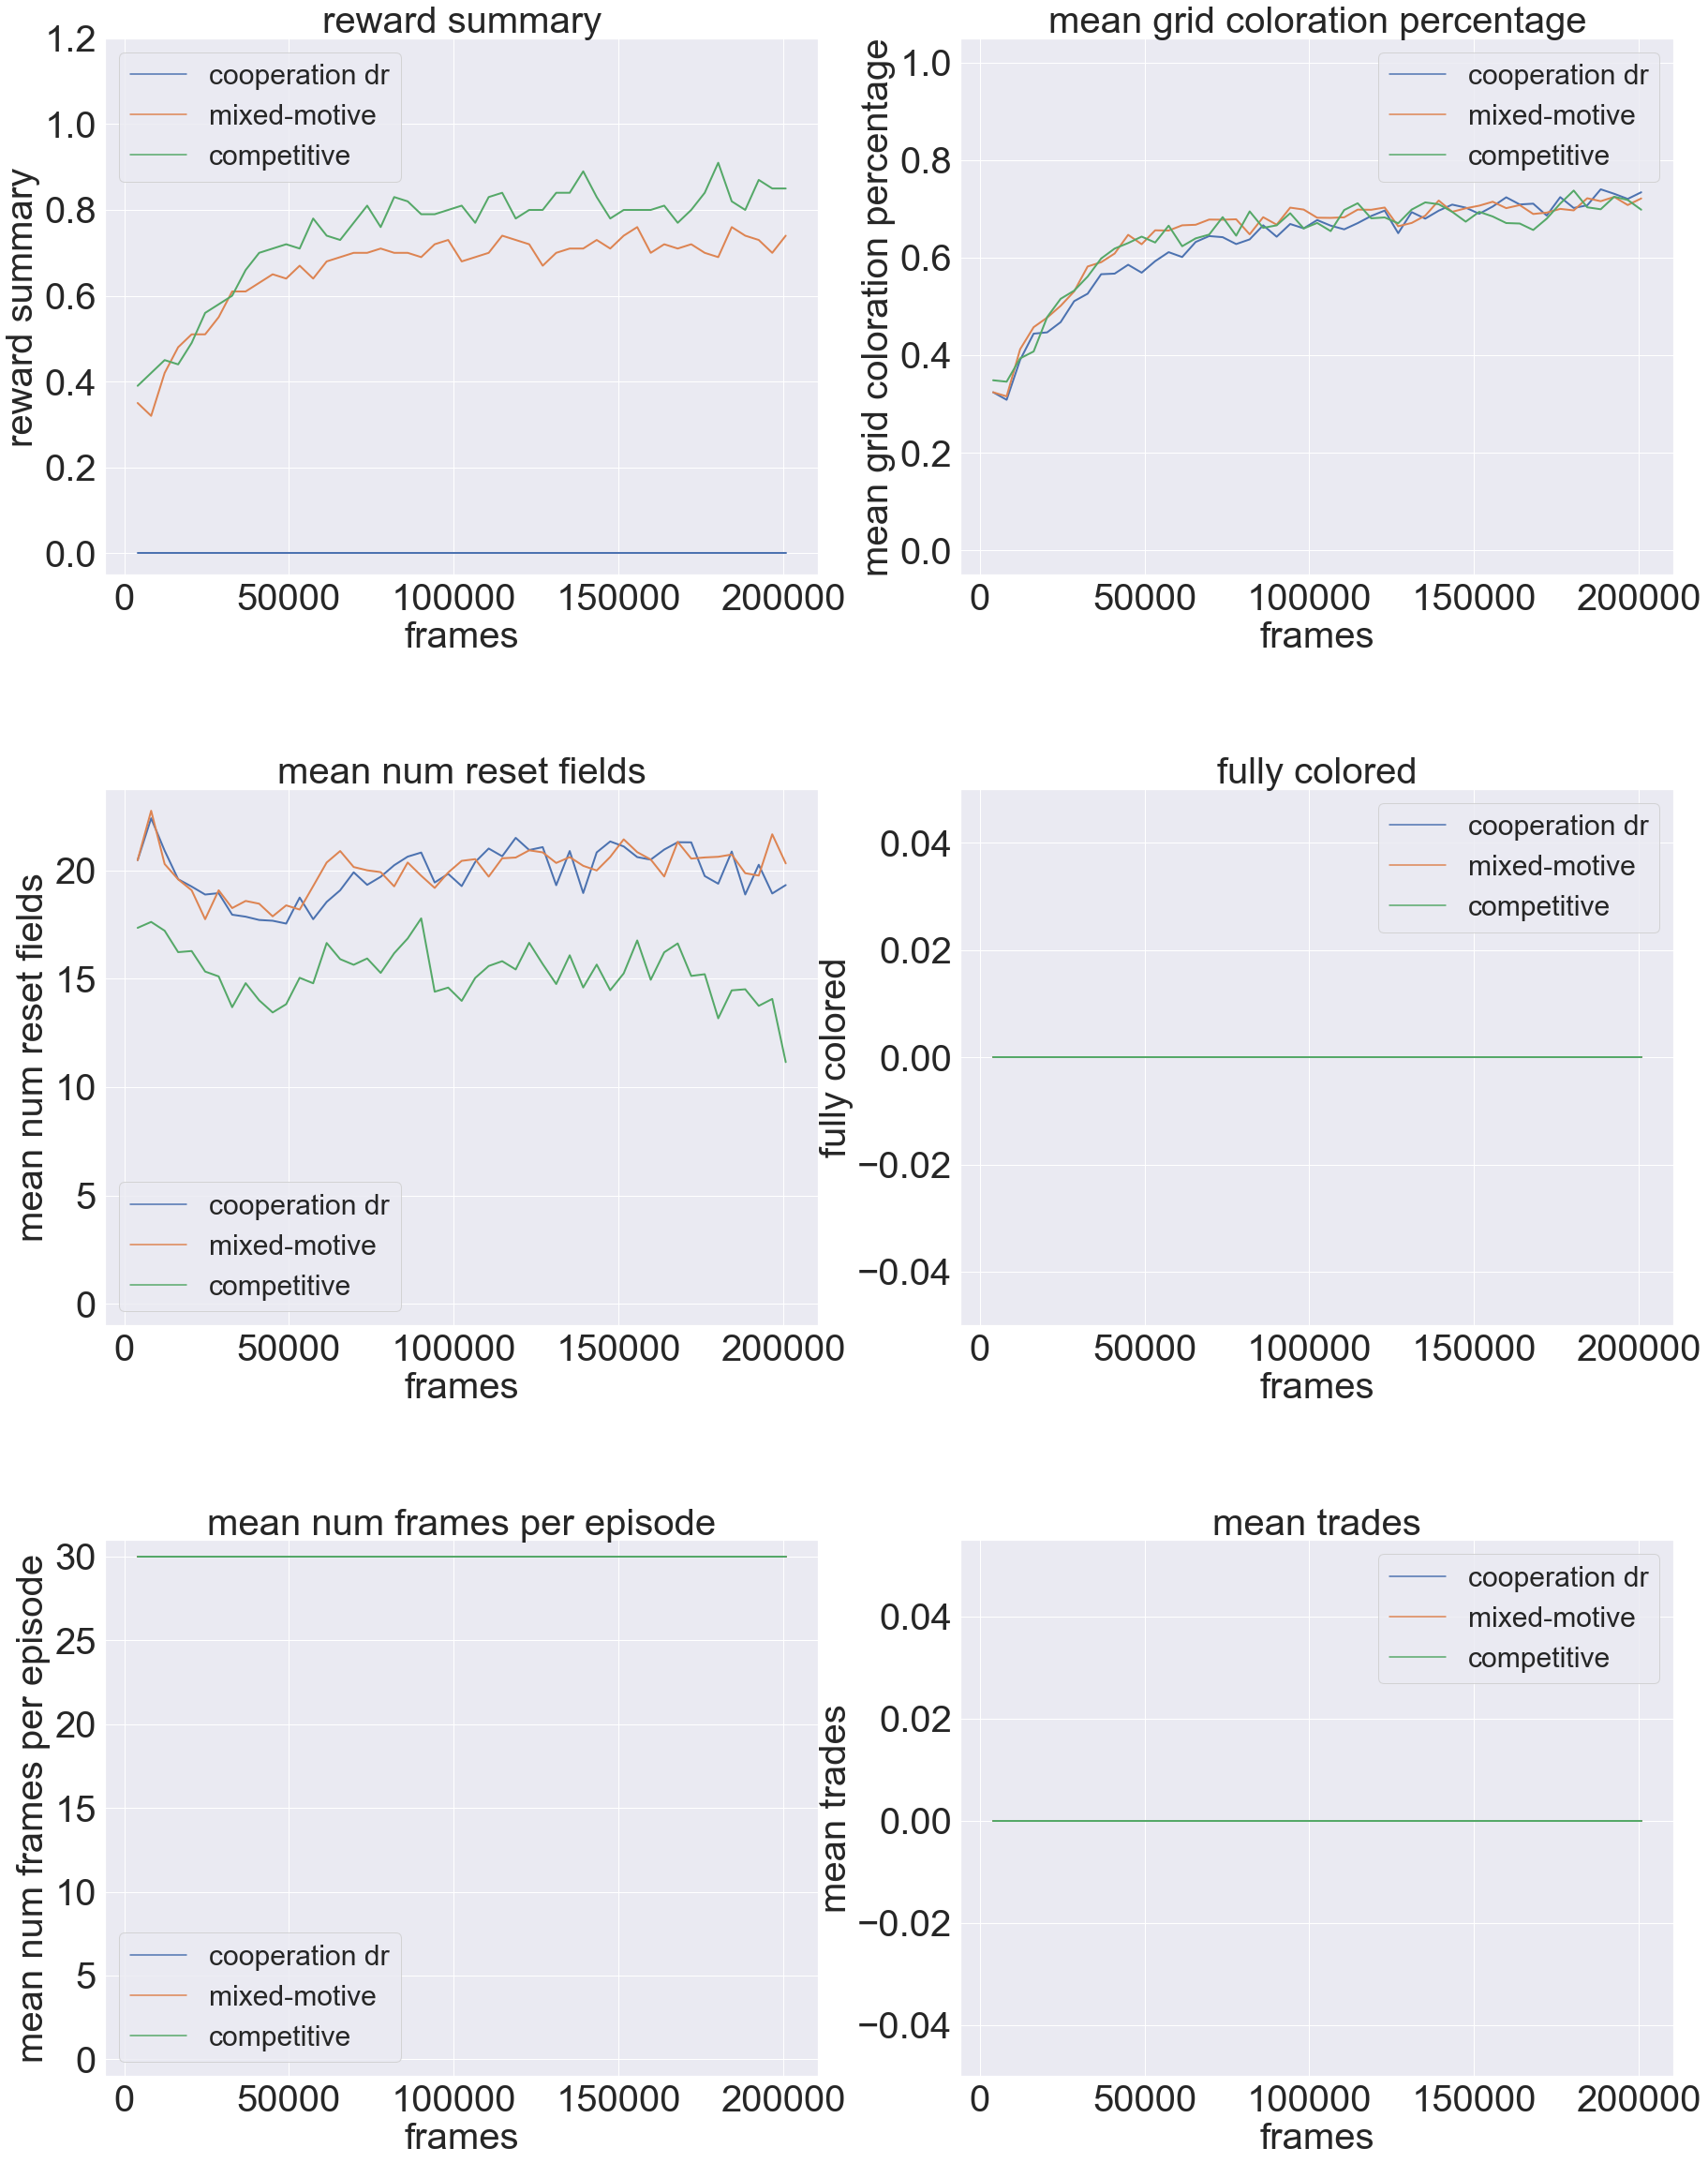
\includegraphics[width=1\textwidth]{AX-rooms-3-ppo.png}\\
    \caption[Training Details of Top PPO Competitive Executions in a Rooms Environment]{Top score details of three PPO agents in a 9x9 Rooms Environment}\label{fig:ax-rooms-3-ppo}
\end{figure}
\vfill
\clearpage


\newpage
\vfill
\begin{figure}
    \centering
    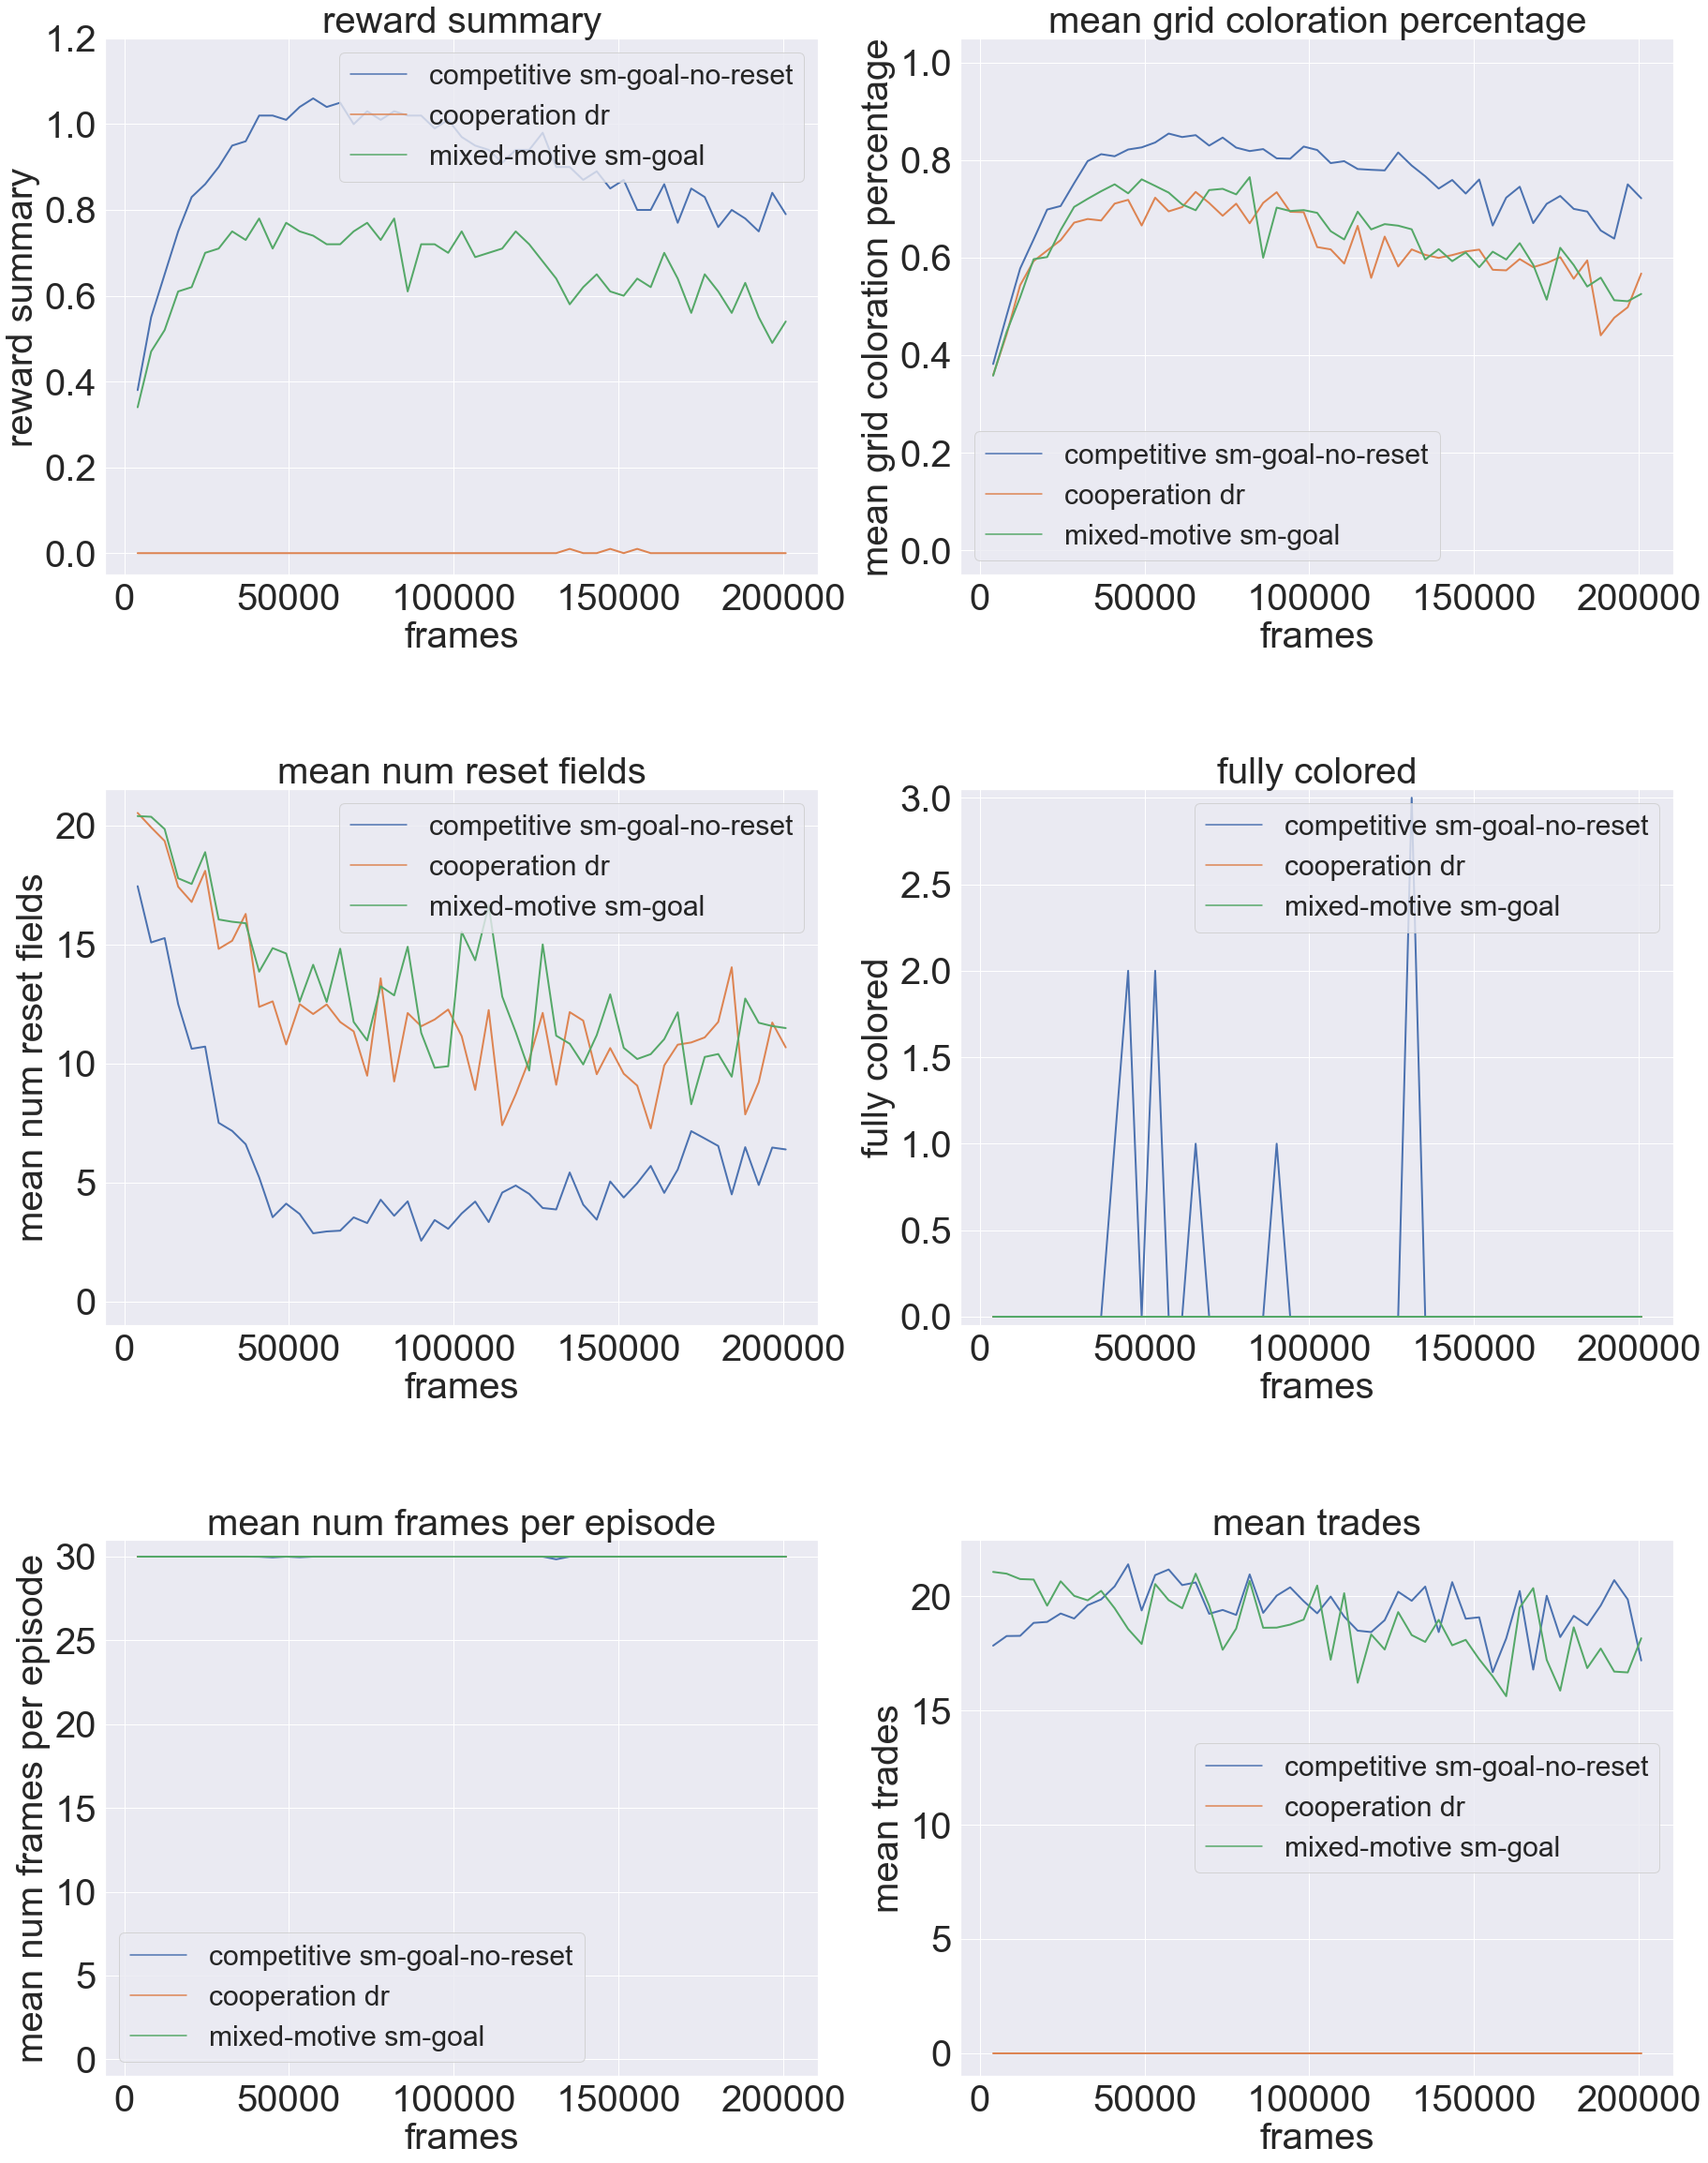
\includegraphics[width=1\textwidth]{AX-rooms-3-dqn.png}\\
    \caption[Training Details of Top DQN Competitive Executions in a Rooms Environment]{Top score details of three DQN agents in a 9x9 Rooms Environment}\label{fig:ax-rooms-3-dqn}
\end{figure}
\vfill
\clearpage

% further appendix
%
% =================================================================================================
% comment \listoffigures and/or \listoftables if not wanted
% -------------------------------------------------------------------------------------------------
%
\backmatter
\listoffigures                                % list of figures (uncomment if wanted)
\listoftables                                 % list of tables (uncomment if wanted)
\lstlistoflistings                            % list of listings (uncomment if wanted)
%
% =================================================================================================
% place your bibliography here
% -------------------------------------------------------------------------------------------------
%
\begin{spacing}{0.9}                          % save some space
    % \bibliographystyle{geralpha}               % for german thesis
    \bibliographystyle{alpha}                 % for english thesis
    \bibliography{bibliography}                % the location of bib file
\end{spacing}
\end{document}
%
% =================================================================================================
% end of document
% -------------------------------------------------------------------------------------------------
%
